\documentclass[times, utf8, diplomski, numeric]{fer}
\usepackage{booktabs}

\usepackage{url}
\usepackage{pdfpages}
\usepackage{subcaption}
\usepackage{listings}
\usepackage[toc,page]{appendix}
\usepackage[ampersand]{easylist}
\usepackage{pdfpages}
\usepackage{pdflscape}

\usepackage{listings}
\lstset{
breaklines=true,
basicstyle=\ttfamily}

\renewcommand{\lstlistingname}{Skripta}
\renewcommand\appendixtocname{Dodaci}
\renewcommand\appendixpagename{Dodaci}

\graphicspath{ {images/} }

\newcommand{\eng}[1]{(engl. \textit{#1})}

\begin{document}

\thesisnumber{1385}

\title{Implementacija kontinuirane isporuke programske podrške za operacijski sustav iOS}

\author{Ivan Rep}

\maketitle

% Ispis stranice s napomenom o umetanju izvornika rada. Uklonite naredbu \izvornik ako želite izbaciti tu stranicu.
\izvornik

% Dodavanje zahvale ili prazne stranice. Ako ne želite dodati zahvalu, naredbu ostavite radi prazne stranice.
\zahvala{Htio bih se zahvaliti izv. prof. dr. sc. Borisu Vrdoljaku na kontinuiranoj potpori i vodstvu kroz diplomski studij}

\tableofcontents

\chapter{Uvod}

Profesionalna izrada programske potpore za iOS operacijski sustav zahtijeva čestu isporuku različitih verzija aplikacije. Osim produkcijske verzije programske potpore, čija učestalost isporuke može varirati od nekoliko puta tjedno do jednom u nekoliko mjeseci, u sklopu razvoja isporučuju se i druge verzije, na primjer verzija koja prikazuje trenutno stanje razvoja i verzija za testiranje. Učestalost isporuke navedenih tipova također značajno varira od tima do tima.

Kako je iOS operacijski sustav relativno mlad, isporuka se još uvijek uglavnom obavlja ručno. Ručna je isporuka programske potpore zahtjevna i podložna ljudskoj pogrešci što dovodi do njenog rijetkog obavljanja.   Rijetko obavljanje isporuke uzrokuje zajedničku isporuku većeg broja promjena što dovodi do lošije kvalitete produkta i sporije isporuke novih funkcionalnosti.

Ovaj je problem moguće riješiti automatizacijom procesa isporuke programske potpore za iOS operacijski sustav. Prije isporuke je programsku potporu potrebno arhivirati a zatim je dobivenu arhivu potrebno objaviti na željenoj platformi. Arhiviranje je proces pripreme iOS projekta za isporuku. Proces arhiviranja i proces objave značajno ovise o platformi na kojoj se objavljuje programsku potporu.

Prije arhiviranja programske potpore potrebno je istu izgraditi te utvrditi zadovoljava li postavljene zahtjeve. Zahtjevi se najčešće izražavaju u obliku testova, ali mogu poprimiti i druge oblike.

Na kraju, potrebno je utvrditi pomoću kojeg je tipa isporuke potrebno isporučiti pojedinu verziju programske potpore.

Navedene se funkcionalnosti mogu svrstati u tri dobro prihvaćene prakse u sklopu računalnog inženjerstva: kontinuiranu integraciju, kontinuiranu dostavu i kontinuiranu isporuku.

Kontinuirana integracija automatizira procese izgradnje, testiranja i osiguranja kvalitete kako bi poboljšala kvalitetu programske potpore. Ovako automatizirani proces provodi se nad svakom novom verzijom programske potpore čime se osigurava njezina ispravnost. Također, kontinuirana integracija potiče učestalu integraciju radnih kopija s glavnom kopijom kako bi se izbjegla pojava konflikta pri integraciji.

Kontinuirana dostava automatizira proces isporuke programske potpore. U sklopu razvoja programske potpore za iOS operacijski sustav, praksa uključuje automatizaciju potpisivanja koda, arhiviranja i objave. Praksa automatiziranjem navedenih procesa nastoji olakšati proces isporuke te tako povećati učestalost objave novih funkcionalnosti. Svaka funkcionalnost koja je razvijena, a nije objavljena, predstavlja gubitak timu. Dokle je god razvijena funkcionalnost neobjavljena, ona ne donosi korist zbog koje je razvijena.

Kontinuirana isporuka automatskom isporukom produkta nastoji što više smanjiti vrijeme proteklo od završetka razvoja do objave funkcionalnosti, pa čak i u potpunosti eliminirati ga. Promjene se ne isporučuju direktno u produkciju već prolaze više faza isporuke. Prvo se isporučuju razvojnom timu, zatim timu za osiguranje kvalitete, vanjskim testerima, a prema potrebi i ograničenom broju stvarnih korisnika. Tek se nakon svih ovih faza promjena isporučuje u produkciju. Kontinuirana integracija ovime nastoji povećati kvalitetu programske potpore, ubrzati isporuku promjena te smanjiti opterećenje razvojnog tima.

U sklopu ovog rada definiram i implementiram navedene prakse za iOS operacijski sustav.

Cilj rada nije samo u teoriji ispitati mogućnost implementacije sustave koji obavlja navedene procese, već ga iskoristiti na stvarnim projektima. Sustav mora biti je jednostavan za implementaciju i korištenje te prenosiva na druge projekte. Zbog ovog ograničenja ne samo da nastojim automatizirati isporuku i integraciju, već nastojim automatizirati i proces dodavanja automatskih procesa projektu.

Rad je strukturiran po praksama redoslijedom koji je korišten u ovom uvodu. Svaku od praksi prvo promatram iz opće perspektive i potom definiram i implementiram za iOS operacijski sustav. Rad završava pregledom ostvarenih funkcionalnosti i zaključkom.


\chapter{Kontinuirana integracija} \label{header:Kontinuirana_Integracija}

Kontinuirana integracija praksa je spajanja razvojnih kopija koda s glavnom kopijom nekoliko puta dnevno. Termin je prvi predložio i iskoristio Grady Booch 1991. godine tijekom opisa metode danas poznate kao Boochova metoda \eng{Booch method}\citep{wiki:BoochMethod}.

Glavni cilj metode jest smanjivanje broja konflikata prilikom spajanja različitih verzija koda. Tijekom razvoja članovi tima preuzimaju zajedničku \eng{master} kopiju izvornog koda \eng{source code} te nad njom obavljaju promjene. Lokalnu kopiju izvornog koda nazivamo \textit{razvojnom kopijom izvornog koda}. Članovi tima pomoću zajedničke kopije izvornog koda stvaraju razvojnu kopiju izvornog koda na vlastitom računalu.

Nakon implementacije željenih promjena programer vlastitu razvojnu kopiju spaja s izvornom kopijom. Ovaj postupak nazivamo integracija izvornog koda. Ako zajednička kopija izvornog koda nije bila mijenjana otkako ju je programer preuzeo, onda je promjene moguće jednostavno dodati zajedničkoj kopiji. Međutim, ako je zajednička kopija izvornog koda izmijenjena, onda je potrebno na neki način spojiti lokalne i promjene koje se već nalaze na glavnoj kopiji izvornog koda.

Što je duže programerova kopija izdvojena, to je veća vjerojatnost da je izvorna kopija u međuvremenu izmijenjena. Što se kopije više razlikuju, to je teže obaviti njihovo spajanje. Ujedno, spajanje često nije moguće obaviti automatski. Ova se pojava naziva konflikt i javlja se prilikom spajanja kopija koje su istovremeno modificirale isti dio istog dokumenta. Programer u takvom slučaju prvo mora preuzeti novu glavnu kopiju, ručno otkloniti konflikte koje prouzrokuju njegove promjene te nakon toga obaviti integraciju.

Nakon nekog vremena izvorna i radna kopija mogu postati toliko različite da je vrijeme potrebno za njihovo spajanje duže od vremena koje je uloženo za implementaciju promjena. Ovaj se problem tada naziva \textit{pakao integracije}. Iako se navedena situacija čini teško mogućom, timovi mogu biti veliki, pritisak može biti visok i tempo naporan. Bez specificiranja postupka verzioniranja te automatizacije izgradnje i provjere ispravnosti projekti lako mogu završiti upravo u navedenom stanju.

Danas je kontinuirana integracija standardna praksa u razvoju programske potpore. Međutim, ona se značajno razlikuje od prakse koju je 1991. godine predložio Grady Booch. Danas se uz kontinuiranu integraciju usko vežu procesi automatizacije izgradnje i testiranja programske potpore. Ovi su pojmovi postali toliko standardan dio kontinuirane integracije da mnogi upravo njih nazivaju kontinuiranom integracijom. Drugim riječima, pojam kontinuirane integracije danas podrazumijeva barem neku razinu automatizacije procesa izgradnje i testiranja. S druge strane, učestalom spajanju radnih kopija daje se malo pozornosti.

Kontinuiranu integraciju moguće je podijeliti na tri generalne faze: izgradnju, testiranje i osiguranje kvalitete. Nadalje, fazu izgradnje moguće je podijeliti na podfaze verzioniranja, pripreme sustava, pripreme ovisnosti i izgradnje projekta. Faze testiranja i osiguranja kvalitete uvelike ovise o tipu programske potpore koja se razvija. U sklopu ovog rada u fazi testiranja provodim unit i UI testove, dok u sklopu faze osiguranja kvalitete provodim provjeru pokrivenosti koda testovima te provjeru izvornog koda korištenjem alata Swiftlint. Podjela kontinuirane integracije na faze s podfazama prikazana je na slici \ref{fig:CIFazes}.

\begin{figure}
\centering
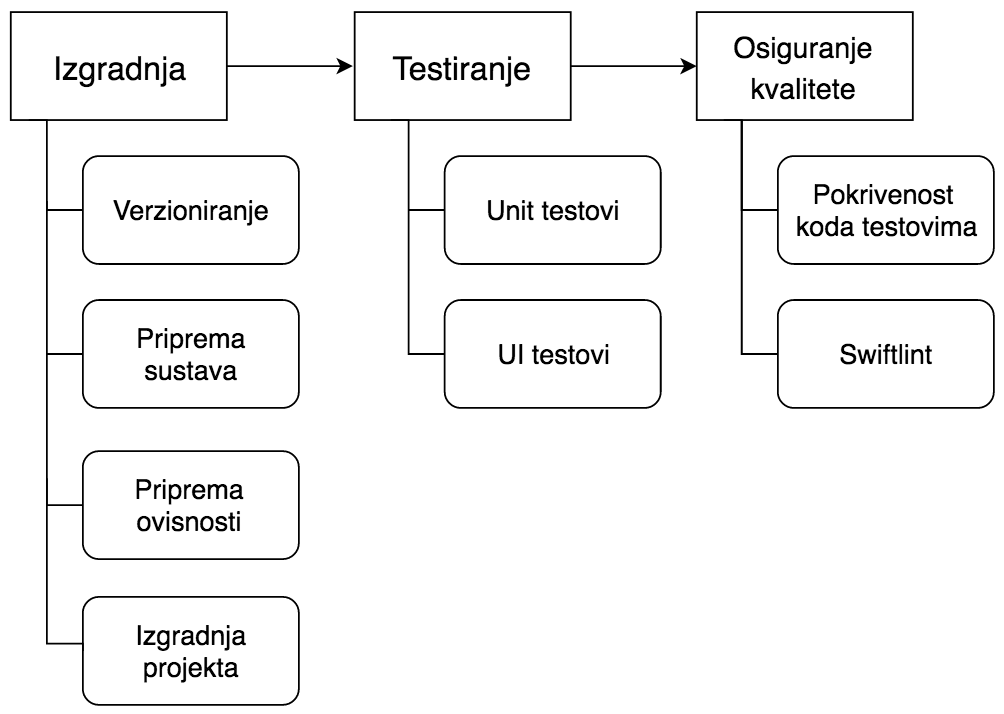
\includegraphics[scale=0.6]{CIFazes}
\caption{Faze kontinuirane integracije}
\label{fig:CIFazes}
\end{figure}

Svaka je faza obrađena zasebnim odlomkom u nastavku poglavlja. Proces verzioniranja u praksi je dio procesa izgradnje, zbog čega je u sklopu odlomka \ref{header:Izgradnja} razmotren i problem učestalosti obavljanja integracije.

Za automatizaciju izgradnje koristim alat Xcode Server. Alat je spoj dvije aplikacije, Xcodea i macOS Servera, te implementira veliki broj funkcionalnosti korištenih u sklopu kontinuirane integracije. Alat se pokazao najboljim među nekoliko sličnih ispitanih alata. Razlog odabira Xcode Server alata detaljnije je prikazan u dodatku \ref{header:dodatak_usporedba_alata_za_kontinuiranu_integraciju}.

\section{Priprema}

Jedan od ciljeva implementacije kontinuirane integracije je i olakšanje cjelokupnog procesa izgradnje, testiranja i osiguranja kvalitete. Što je implementacija automatizacije zahtjevnija, to se više narušava navedeni cilj. Zbog navedenog nastojim automatizirati instalaciju i konfiguraciju što većeg broja alata i tako olakšati cjelokupan proces implementacije kontinuirane integracije. Također, automatizacija procesa instalacije i konfiguracije pruža veću kontrolu nad samim procesom. Na primjer, alat je moguće instalirati samo kad je potreban i ako je uopće potreban, dok se ručnim postupkom instalacija alata mora obaviti prije pokretanja automatizacije.

MacOS je vrlo siguran, a zbog toga i zatvoren operacijski sustav. Veliki broj alata zahtijeva korisničku interakciju zbog čega je njihovu instalaciju teško automatizirati. Dodatno, ako se instalacija obavlja za više računa operacijskog sustava ili alat pristupa osjetljivim datotekama, onda je instalaciju potrebno autorizirati lozinkom računa s administracijskim privilegijama. Postoji nekoliko načina za automatski upis lozinke, ali navedeni procesi narušavaju sigurnost operacijskog sustava te zbog toga nije moguće u potpunosti automatizirati proces dohvata i pripreme alata.

Ovaj odlomak prikazuje pripremu alata čiju instalaciju nije moguće automatizirati, dok odlomak \ref{header:PripremaSustava} prikazuje pripremu ostalih alata. Primjeri su napisani za macOS operacijski sustav te su testirani na \textit{Sierra 10.12.4} verziji. Minimalna preporučena verzija operacijskog sustava je \textit{Yosemite 10.10}.

Za implementaciju kontinuirane integracije koristim brojne alate koji ne pružaju vizualno korisničko sučelje. Navedenim se alatima pristupa korištenjem naredbenog korisničkog sučelja - \textit{ljuske}. U sklopu rada koristim \textit{bash} ljusku. Pristup naredbenom korisničkom sučelju ostvaruje se korištenjem emulatora terminala - aplikacija s vizualnim sučeljem koje emuliraju terminal. U radu koristim aplikaciju \textit{Terminal} koja je dostupna u sklopu instalacije macOS operacijskog sustava.

\subsection{Xcode Server}

\begin{figure}
\centering
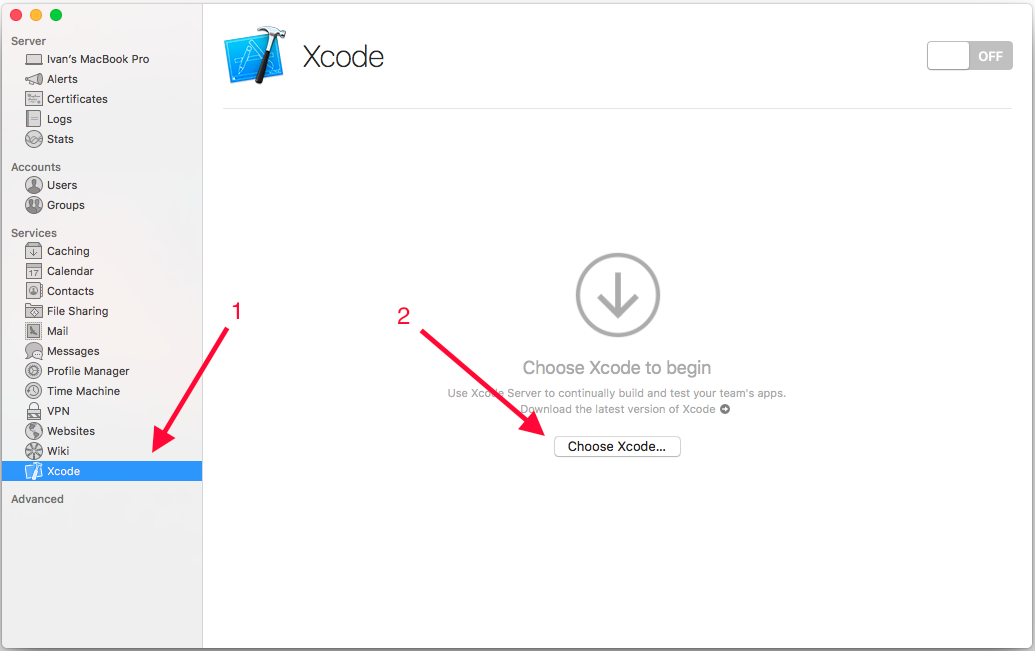
\includegraphics[scale=0.35]{XcodeServerSetup1}
\caption{Povezivanje macOS Server i Xcode aplikacija}
\label{fig:XcodeServerSetup1}
\end{figure}

Xcode Server spoj je dvije aplikacije - Xcodea i macOS Servera. Xcode je integrirani sustav za razvoj programske potpore za iOS, macOS, tvOS i watchOS operacijske sustave. MacOS Server je alat za automatizaciju procesa na macOS operacijskom sustavu. Prije implementacije kontinuirane integracije potrebno je preuzeti, instalirati i konfigurirati obje aplikacije.

Moguće je oba alata preuzeti korištenjem App Store aplikacije koja je dostupna u sklopu svake instalacije macOS operacijskog sustava. Međutim, cijena macOS Server aplikacije u trenutku pisanja ovog rada iznosi \$25. Aplikacija je besplatna za korisnike s Apple Developer računom koji se koristi i u razvoju iOS programske potpore. Besplatnu verziju macOS Servera moguće je preuzeti na poveznici \path{https://developer.apple.com/download/}. Nakon preuzimanja potrebno je slijediti upute za instalaciju obje aplikacije.

\begin{figure}
\centering
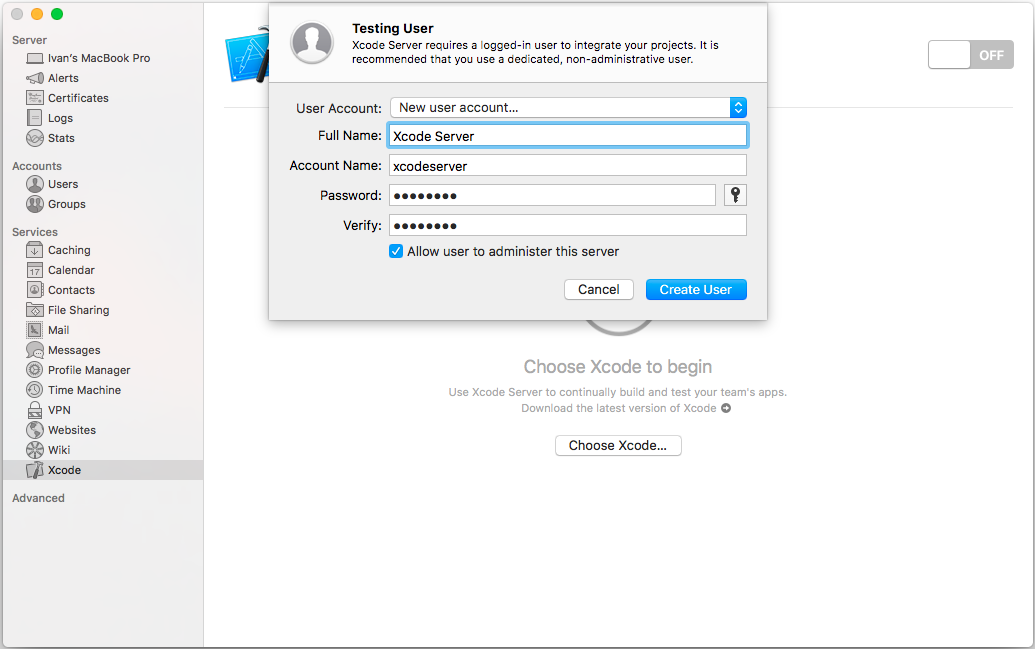
\includegraphics[scale=0.35]{XcodeServerSetup2}
\caption{Kreiranje xcodeserver korisničkog računa}
\label{fig:XcodeServerSetup2}
\end{figure}

Nakon instalacije alata potrebno je kreirati Xcode Server alat povezivanjem Xcode i macOS Server aplikacija. Pokrenuti macOS Server i u lijevom bočnom izborniku odabrati opciju \verb|Xcode -> Choose Xcode...|. U novootvorenom izborniku potom je potrebno odabrati željenu verziju Xcode aplikacije. Slika \ref{fig:XcodeServerSetup1} prikazuje proces povezivanja macOS Server i Xcode aplikacija.

\begin{figure}[b!]
\centering
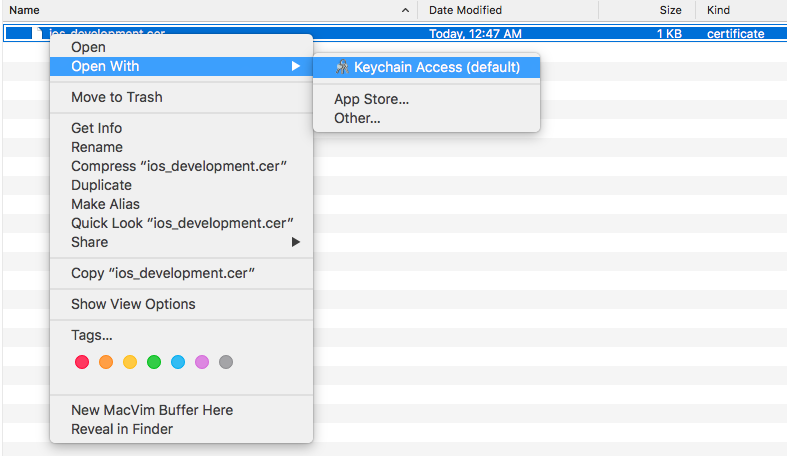
\includegraphics[scale=0.4]{DodavanjeCertifikata}
\caption{Dodavanje certifikata korištenjem Keychain Access aplikacije}
\label{fig:DodavanjeCertifikata}
\end{figure}

Preporučeno je zbog sigurnosnih razloga macOS Server pokrenuti na zasebnom računu operacijskog sustava te mu omogućiti korištenje samo potrebnih alata i datoteka. Nakon povezivanja Xcode aplikacije s macOS Serverom, otvara se izbornik u kojem je moguće kreirati novi račun operacijskog sustava ili odabrati postojeći. U sklopu ovog rada kreiram novi račun predodređenog imena \textit{xcodeserver}. Slijediti upute nakon kreiranja računa za dovršetak spajanja aplikacija.

Proces potpisivanja koda osigurava autentičnost i neizmjenjenost kreirane programske potpore. Proces je detaljnije objašnjen u \ref{header:PotpisivanjeKoda} odlomku. Za sada je dovoljno znati da proces zahtijeva postojanje tri artefakta: certifikat člana tima, identifikator aplikacije i pripremni profil aplikacije za tip isporuke koji se koristi. Navedene artefakte moguće je kreirati i preuzeti s web stranice \path{https://developer.apple.com/account}.

Certifikat i identifikator instaliraju se korištenjem Keychain Access aplikacije. Dovoljno ih je pokrenuti korištenjem navedene aplikacije. Pripremne profile potrebno je spremiti na lokaciji \path{~/Library/MobileDevice/Provisioning_Profiles} računa koji obavlja integraciju.

Xcode Server automatizaciju izgradnje, testiranja i isporuke ostvaruje korištenjem alata imena \textit{bot}. \textit{Bot} se kreira i konfigurira korištenjem Xcode aplikacije, a pokreće na macOS Server aplikaciji. Navedene aplikacije ne moraju se nalaziti na istom računalu, ali moraju biti povezane.

Pokrenuti željeni projekt korištenjem aplikacije Xcode. Prozor za kreiranje \textit{bota} pokreće se odabirom opcije \textit{Product -> Create bot}. U novootvorenom prozoru imenovati bot te odabrati macOS Server aplikaciju na kojoj će se bot izvršavati. Ako macOS Server nije vidljiv, potrebno je ponovno pokrenuti macOS Server aplikaciju i provjeriti povezanost s Xcode aplikacijom. Slika \ref{fig:BotServerSelection} prikazuje odabir macOS Server aplikacije kod kreiranja bota.

\begin{figure}
\centering
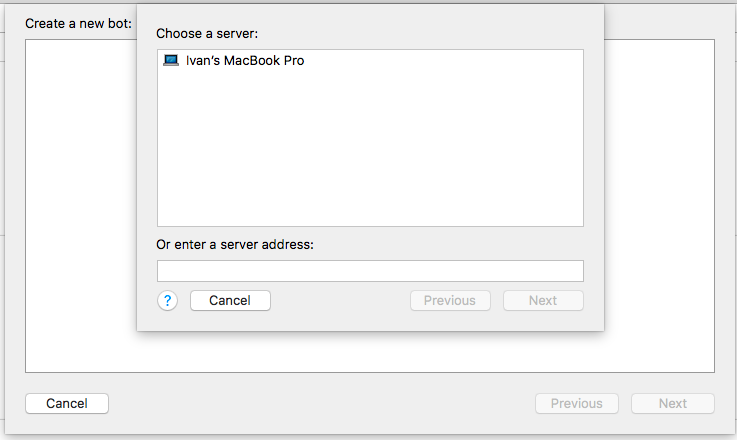
\includegraphics[scale=0.4]{BotServerSelection}
\caption{Odabir macOS Server aplikacije za obvljanje kontinuirane integracije}
\label{fig:BotServerSelection}
\end{figure}

\subsection{Homebrew}

Homebrew je alat za dohvat i upravljanje alatima za macOS operacijski sustav\citep{homebrew}. Također, alat navedene funkcionalnosti pruža korištenjem naredbenog korisničkog sučelja zbog čega ih je jednostavno automatizirati. Instalacija alata zahtijeva administrativna prava \eng{sudo user}, zbog čega istu nije moguće automatizirati. Skripta \ref{listing:homebrew} instalira Homebrew alat korištenjem \textit{ruby} alata. Nakon pokretanja naredbe slijediti upute instalacije.

\begin{lstlisting}[caption=Instalacija Homebrew alata, label=listing:homebrew]
ruby -e "$(curl -fsSL https://raw.githubusercontent.com/Homebrew/install/master/install)"
\end{lstlisting}

\section{Izgradnja} \label{header:Izgradnja}

Povijesno, pojam izgradnja često se koristio kao sinonim za kompajliranje. Kompajliranje \eng{compilation} je proces prevođenja koda iz izvornog u ciljni jezik uz očuvanje funkcionalnosti. Kod se uz prevođenje često i optimizira. Najčešći razlog kompajliranja je prevođenje koda u jezik koji procesor može razumjeti i tako ga izvršiti. Rezultat ovog tipa kompajliranja jest izvršni program, odnosno program koji se može izvršiti. Kompajliranje je složena funkcija koja se najčešće obavlja u više prolaza. Jezici koji se kompajliraju se nazivaju kompajlirani jezici \eng{compiled languages}.

Interpretirani jezici \eng{interpreted languages} se ne prevode već interpretiraju. Oni se izvršavaju na pomoćnom programu naziva interpreter koji naredbe izvornog jezika prevodi i izvršava. Danas gotovo niti jedan jezik nije u cijelosti kompajliran ili interpretiran, već koristi kombinaciju obje metode s ciljem poboljšanja performansi.

\begin{figure}[b!]
\centering
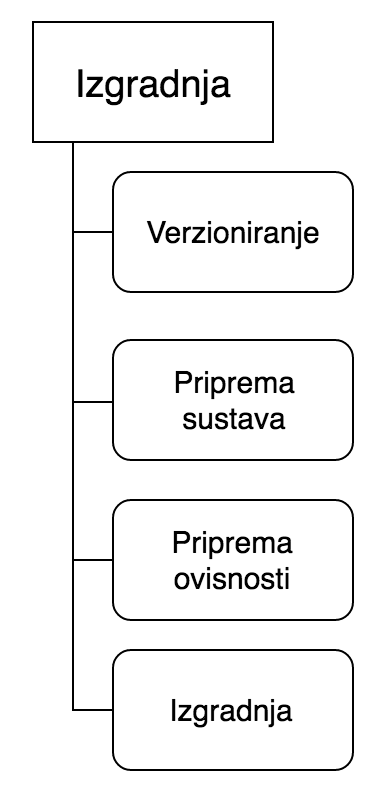
\includegraphics[scale=0.5]{BuildProcess}
\caption{Podfaze procesa izgradnje}
\label{fig:BuildProcess}
\end{figure}

Danas se s pojmom izgradnje vežu svi procesi koji su dio pretvaranja izvornog koda u željeni artefakt. Ovisno o jeziku i alatima koji se koriste, proces izgradnje može značajno oscilirati u svojoj veličini i složenosti. Generalno, proces izgradnje možemo podijeliti na verzioniranje, pripremu sustava za izgradnju, dohvat i pripremu ovisnosti \eng{dependencies} te kompajliranje. Verzioniranjem odabiremo željenu verziju izvornog koda koju koristimo za izgradnju artefakta. Priprema za izgradnju dovodi računalo u stanje potrebno za obavljanje izgradnje. Izvorni kod često sadržava upute za pripremu sustava kao što su potrebni alati i postavke projekta. Dohvat i priprema ovisnosti osigurava postojanje ovisnosti koje zahtijeva izvorni kod. Ovisnosti dijelimo na dva tipa: ovisnosti koje su dio razvojne okoline i vanjske \eng{third party} ovisnosti, koje uglavnom razvija zajednica. Kompajliranje prevodi izvorni kod u izvršivi artefakt. Kod interpretiranih jezika ovaj je proces često zamijenjen statičkom i dinamičkom provjerom izvedivosti programa. Zbog jednostavnijeg sporazumijevanja, oba procesa nazivam izgradnja projekta. Slika \ref{fig:BuildProcess} prikazuje podjelu procesa izgradnje.

Osim kreiranja artefakta, izgradnja provjerava i je li verzija izvornog koda izgradiva. Kod je izgradiv ako u procesu izgradnje ne izaziva pogrešku, odnosno ako se kod ispravno izgradi. Pogrešku može izazvati neispravnost u izvornom kodu, neispravna konfiguracija sustava, nepostojanje potrebnog alata ili neki drugi nedostatak. Izgradivost sustava preduvjet je za testiranja i isporuku. Samim time automatizacija izgradnje preduvjet je za automatizaciju testiranja i automatizaciju isporuke.

\subsection{Verzioniranje} \label{header:Verzioniranje}

Verzioniranje je proces dodjele jedinstvene oznake \eng{id} stanju repozitorija. Repozitorij je verzioniran direktorij i može sadržavati sve od izvornog koda do certifikata i izvršnog programa. Jedinstvena oznaka omogućava identifikaciju pojedinog stanja repozitorija i izgradnju stabla promjena \eng{source tree} koje povezivanjem stanja prikazuje povijest izmjena repozitorija. Verzionirano stanje repozitorija se naziva verzija \eng{commit}\citep{wiki:SoftwareVersioning}.

\begin{figure}[b!]
\centering
\begin{subfigure}{.24\textwidth}
\centering

\includegraphics[scale=0.4]{VersioningTreeA}
\caption{Glavni repozitorij}
\label{fig:VersioningTreeA}
\end{subfigure}
\begin{subfigure}{.24\textwidth}
\centering

\includegraphics[scale=0.4]{VersioningTreeB}
\caption{Repozitorij A}
\label{fig:VersioningTreeB}
\end{subfigure}
\begin{subfigure}{.24\textwidth}
\centering

\includegraphics[scale=0.4]{VersioningTreeC}
\caption{Repozitorij B}
\label{fig:VersioningTreeC}
\end{subfigure}
\begin{subfigure}{.24\textwidth}
\centering
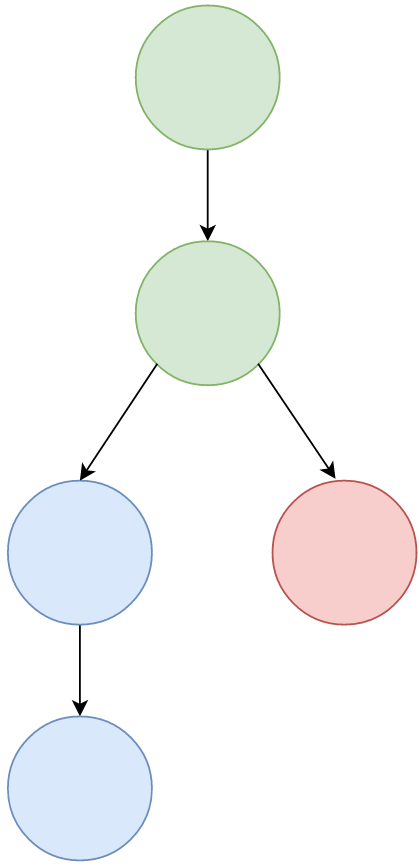
\includegraphics[scale=0.4]{VersioningTree}
\caption{Spojeni prikaz}
\label{fig:VersioningTreeD}
\end{subfigure}
\caption{Stablo promjena}
\label{fig:VersioningTree}
\end{figure}

Uz jedinstvenu oznaku i stanje repozitorija, proces verzioniranja pohranjuje i dodatne podatke kao što su autor i datum kreiranja verzije te identifikator prijašnje verzije. Navedeni podaci omogućavaju izgradnju stabla promjena. Dodatno, ako se verzije poredaju kronološki po datumu obavljanja izmjena, onda svaka pojedina verzija ne treba sadržavati cijelo stanje repozitorija. Dovoljno je samo navesti promjene obavljene nakon prijašnje verzije. Navedeni proces ne samo da značajno smanjuje veličinu cijele kopije, već olakšava i praćenje izmjena. Slika \ref{fig:VersioningTree} prikazuje primjer stabla promjena. Glavni repozitorij sadrži dvije verzije. Repozitorij u navedenom stanju preuzimaju dva člana tima čime kreiraju lokalne repozitorije nad kojima obavljaju izmjene. Globalno stablo promjena kreira se zajedničkim prikazom stabla promjena svih članova.

Navedeni se tip verzioniranja naziva inkrementalno verzioniranje, jer se zbog lakšeg praćenje promjena provodi vrlo često. Identifikatori ovog tipa verzioniranja najčešće su generirani pseudo-slučajno. U praksi se često koriste i dodatne sheme verzioniranja koje olakšavaju praćenje stanja projekta. Navedene sheme nastoje olakšati praćenje projekta zbog čega se ovaj tip verzioniranja naziva vanjsko verzioniranje. Nove verzije se kreiraju dodavanjem posebnih oznaka postojećoj verziji inkrementalnog verzioniranja. Na primjer, u praksi je standardno označiti svaku verziju iz koje se kreira produkt posebnom oznakom koja se naziva verzija izgradnje \eng{build number}. Kako vanjsko verzioniranje nosi neko značenje, proces dodjele identifikatora puno je složeniji i ovisi o svrsi koje se pokušava postići.

Unutarnje verzioniranje koda naziva se kontrola verzija\citep{wiki:VersionControl}. Sustavi koji implementiraju proces kontrole verzija nazivaju se sustavi za kontrolu verzija. Kroz povijest je razvijen veliki broj sustava za kontrolu verzija, a danas je timski razvoj programske potpore gotovo nezamisliv bez korištenja jednog od njih.

Danas su u praksi najpopularnija dva alata: Apach Subversion i git.

Apache Subversion, poznat i pod skraćenicom svn, kreiran je 2000. godine u sklopu projekta koji je vodila \textit{Apache Software Foundation} zajednica. Alat je centraliziran, siguran i jednostavan za korištenje te je danas objavljen kao alat otvorenog koda. Generalno, postoji jedan glavni repozitorij koji članovi tima kloniraju, uređuju te zatim lokalne promjene sinkroniziraju s njim.

Git je kreirao Linus Torvalds 2005. godine zbog nezadovoljstva tadašnjim sustavima za kontrolu verzija. Git je izdan kao alat otvorenog koda te je ubrzo okupio veliku podršku u zajednici. Za razliku od svn-a, git je distribuirani sustav. Repozitoriji istog projekta mogu postojati na proizvoljnom broju uređaja u proizvoljnom broju stanja. Navedeni se repozitoriji mogu klonirati, usklađivati i uređivati neovisno jedan o drugom. Zbog navedenog, pomoću gita moguće je implementirati proizvoljan pristup verzioniranju, bio to centralizirani repozitorij nalik na svn-ov pristup, pristup s osobama zaduženim za odobravanje promjena, distribuirani model ili drugo. Najvažnije, git je jednostavan ali vrlo moćan alat. Implementacija osnovnih funkcionalnosti intuitivna je dok istovremeno postoji podrška za vrlo kompleksne pothvate.

Svn je stariji, međutim još uvijek široko korišten sustav. Koristi ga veliki broj starijih kompanija i projekata otvorenog koda. Git je značajno popularniji na novijim projektima, posebno onim otvorenog koda. Njegova jednostavnost i fleksibilnost čine ga lakšim za upoznavanje i korištenje. Zbog toga u ovom rada koristim git. Sve se funkcionalnosti mogu, uz manju modifikaciju, implementirati i korištenjem svn-a.

\paragraph{Uvod u git}

Temeljne funkcionalnosti git alata su repozitoriji i grane. Repozitorij je direktorij koji je verzioniran korištenjem git sustava za kontrolu verzija. Ovaj repozitorij sadrži direktorij \verb|.git| koji specificira na koji se način verzionira direktorij te sadrži informacije o repozitoriju.

Repozitoriji se mogu klonirati na istom ili drugom uređaju. Klonirani repozitorij je novi repozitorij identičan izvornom repozitoriju. Promjene koje se obavljaju u kloniranom repozitoriju nemaju nikakvog utjecaja na izvorni repozitorij. Međutim, promjene obavljene u kloniranom repozitoriju se mogu, uz postojanje odgovarajuće autorizacije, prenijeti na izvorni repozitorij. Prijenos promjena se ne mora obavljati isključivo između izvornog i kloniranog repozitorija, već se može obaviti između bilo koja dva povezana repozitorija.

\begin{figure}[b!]
\centering
\begin{minipage}{.5\textwidth}
\centering
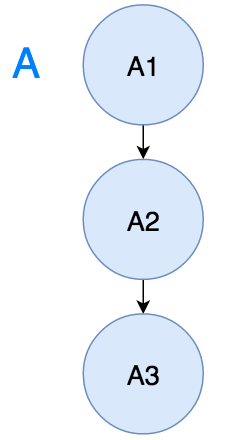
\includegraphics[scale=0.6]{Initial_commit}
\caption{Grana s tri potvrde}
\label{fig:Initial_commit}
\end{minipage}%
\begin{minipage}{.5\textwidth}
\centering
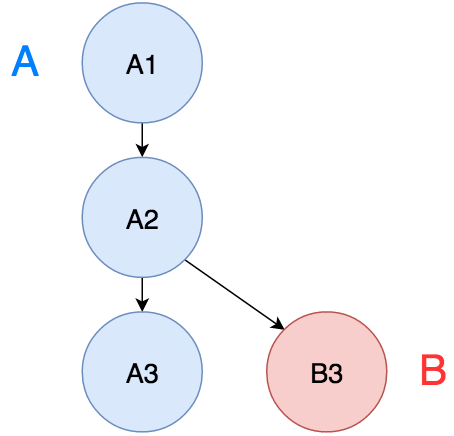
\includegraphics[scale=0.6]{Branching}
\caption{Grananje}
\label{fig:Branching}
\end{minipage}
\end{figure}

Prilikom kreiranja git repozitorija stvara se i glavna grana (engl. master branch) repozitorija. Grana je definirana slijedom verzija koje su obavljene na njoj. Stvaranje nove verzije na trenutnoj se grani ostvaruje potvrđivanjem promjena \eng{commit} koje su dodane repozitoriju. Potvrđivanje promjena prikazano je na slici \ref{fig:Initial_commit}. Repozitorij koda stvara se kreiranjem glavne grane i obavljanjem inicijalnog potvrđivanja \eng{initial commit}. Glavna grana označena je slovom A. Inicijalno potvrđivanje označeno je identifikatorom A1, dok su naknadna potvrđivanja označena identifikatorima A2 i A3.

\begin{figure}
\centering
\begin{subfigure}{.49\textwidth}
\centering
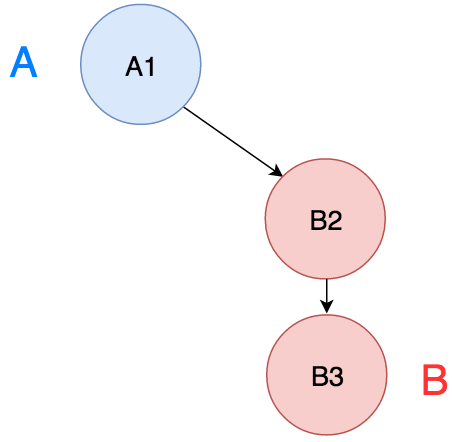
\includegraphics[scale=0.6]{FastForwardA}
\caption{Stanje prije spajanja}
\label{fig:FastForwardA}
\end{subfigure}
\begin{subfigure}{.49\textwidth}
\centering
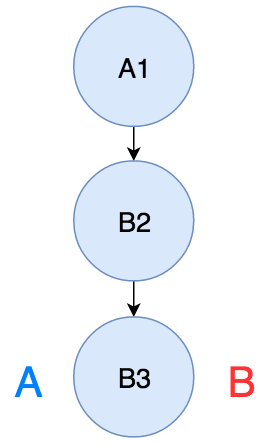
\includegraphics[scale=0.6]{FastForwardB}
\caption{Stanje nakon spajanja}
\label{fig:FastForwardB}
\end{subfigure}
\caption{Spajanje dodavanje promjena}
\label{fig:FastForward}
\end{figure}

Nova se grana može kreirati iz bilo kojeg stanja postojeće grane. Ovaj se postupak naziva grananje \eng{branching}. Izvorna i kreirana grana dijele zajedničku povijest do trenutka grananja. Daljnje promjene primjenjuju se samo na jednu od postojećih grana. Slika \ref{fig:Branching} prikazuje postupak grananja. Grana B se kreira iz stanja A2 grane A. Grane A i B dijele dva zajednička stanja A1 i A2. Ova stanja nazivamo zajednička povijest grana A i B. Nakon grananja na granu B dodaje se novo stanje B3.

Grane je također moguće spojiti. Spajanje grana dodaje promjene obavljene na izvornoj \eng{source} grani u odredišnu \eng{destination} granu. Spajanje je moguće obaviti na nekoliko načina ovisno o odnosu dviju grana koje se spajaju. Slika \ref{fig:FastForward} prikazuje najjednostavniji odnos dviju grana kod spajanja. Nakon grananja grane B iz stanja A1 grane A na granu B se dodaju dva nova stanja, B2 i B3. U međuvremenu je grana A ostala nepromijenjena. Zbog navedenog spajanje grana moguće je obaviti jednostavno dodavanjem promjena B grane na vrh A grane, \eng{fast forward merge}. Slike \ref{fig:FastForwardA} prikazuje stanje prije spajanja dok slika \ref{fig:FastForwardB} prikazuje stanje nakon spajanja. Također, samo je spajanje moguće označiti dodavanjem novog stanja na odredišnu granu.

Postupak se komplicira ako je odredišna grana modificirana nakon grananja. U navedenom slučaju nije moguće promjene obavljene u izvorišnoj gani samo dodati na vrh odredišne grane, nego je promjene potrebno spojiti. Proces spajanja ovisi o tome postoje li konflikti između promjena. Ako ne postoji, spajanje je moguće obaviti jednako kao na slici \ref{fig:FastForward}, jednostavno dodavanjem promjena na vrh odredišne grane.

\begin{figure}
\centering
\begin{subfigure}{.49\textwidth}
\centering
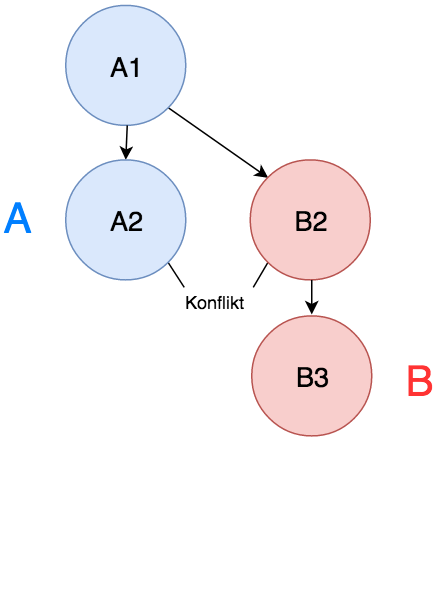
\includegraphics[scale=0.6]{ConflictA}
\caption{Stanje prije spajanja}
\label{fig:ConflictA}
\end{subfigure}
\begin{subfigure}{.49\textwidth}
\centering
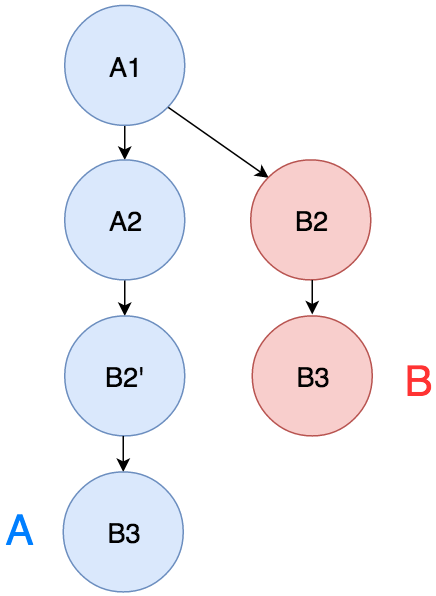
\includegraphics[scale=0.6]{ConflictB}
\caption{Stanje nakon spajanja}
\label{fig:ConflictB}
\end{subfigure}
\caption{Spajanje otklananjem konflikta}
\label{fig:Conflict}
\end{figure}

Međutim, ako promjene izazivaju konflikte, onda je te konflikte potrebno ručno razriješiti. Otklanjanje konflikata uzrokuje izmjenu verzija jedne ili obje grane. Proces otklanjanja konflikata najčešće se odrađuje dodavanjem jedne po jedne verzije izvorne grane na odredišnu granu. Ako izvorna verzija ne izaziva konflikt, ona se jednostavno dodaje na vrh odredišne grane. Međutim, ako verzija izaziva konflikt, tada se isti otklanja modificiranjem iste. Slika \ref{fig:Conflict} prikazuje proces spajanja grana s konfliktom. Konflikt je nastao između verzija A2 i B2. Konflikt se otklanja dodavanjem verzije B2 na vrh A grane i njenim modificiranjem. Ovo je stanje označeno s B2'. Stanje B3 ne izaziva konflikt te se samo dodaje na vrh A grane. Rezultat spajanja su dvije grane A i B različitih povijesti.

\begin{figure}[b!]
\centering
\begin{subfigure}{.3\textwidth}
\centering
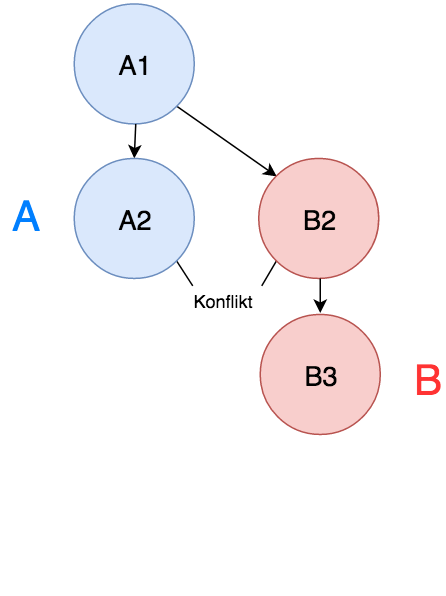
\includegraphics[scale=0.5]{RebaseA}
\caption{Početno stanje}
\label{fig:RebaseA}
\end{subfigure}
\begin{subfigure}{.3\textwidth}
\centering
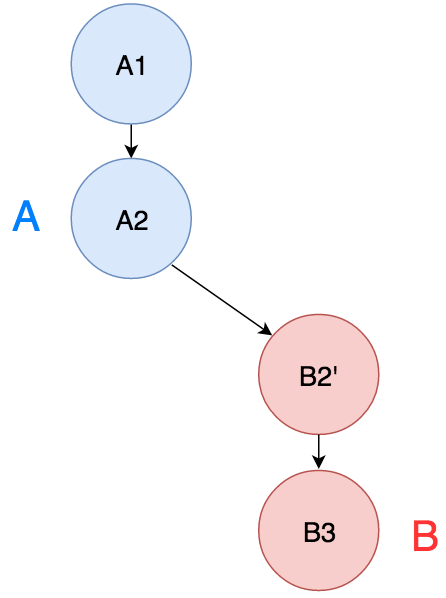
\includegraphics[scale=0.5]{RebaseB}
\caption{Stanje nakon \textit{rebase}}
\label{fig:RebaseB}
\end{subfigure}
\begin{subfigure}{.3\textwidth}
\centering
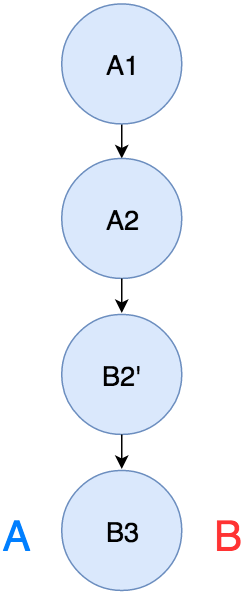
\includegraphics[scale=0.5]{RebaseC}
\caption{Stanje nakon spajanja}
\label{fig:RebaseC}
\end{subfigure}
\caption{Spajanje \textit{rebase} postupkom}
\label{fig:Rebase}
\end{figure}

Isti je slučaj moguće riješiti postupkom koji se naziva \textit{rebase}. Postupak prije spajanja u povijest izvorišne grane dodaje sve verzije nastale u odredišnoj grani nakon grananja. Verzije se dodaju odmah nakon stare točke grananja čime se točka grananja pomiče na zadnju trenutnu verziju A grane. Slika \ref{fig:RebaseB} prikazuje stanje nakon obavljanja \textit{rebase} postupka na grani B. Sada su grane u stanju jednakom onom na slici \ref{fig:FastForward} te je spajanje moguće obaviti dodavanjem promjena na vrh odredišne grane. Stanje B2 se još uvijek mijenja, međutim, sada je povijest repozitorija linearna.

\paragraph{Tijek verzioniranja} \label{header:Implementacija_verzioniranja}

Ostaje otvoreno pitanje kako koristiti alat za kontrolu verzija. Koliko često kreirati novu verziju koda i koliko često promjene spajati sa zajedničkim repozitorijem? Kod korištenja gita javljaju se i pitanja kako organizirati repozitorije i sustav grananja.

Programer koji samostalno radi na projektu najčešće koristi jedan javni repozitorij s jednom granom na kojoj obavlja promjene i proizvoljno sinkronizira lokalni s glavnim repozitorijem. Međutim, ovaj je pristup vrlo teško održiv u timskom radu. Učestalo preplitanje različitih tokova razvoja na jednoj grani značajno otežava praćenje razvoja i čini teškim poništavanje neželjenih promjena.

Danas se u praksi koristi nekoliko različitih tijeka rada verzioniranja \eng{versionining workflows}. Ovaj odlomak obrađuje centralizirani tijek rada \eng{centralized workflow}, tijek rada grananja funkcionalnosti \eng{feature branch workflow}, \textit{gitflow} tijek rada \eng{gitflow workflow} i tijek rada izdvajanja promjena \eng{forking workflow}. Svaki od navedenih pristupa ima svoje prednosti i mane te se koristi u različitim tipovima projekta\citep{versioningWorkflows}.

Centralizirani tijek rada koristi jedan glavni i više lokalnih repozitorija. Najčešće se koristi samo jedna, glavna grana. Svaki programer kreira lokalnu kopiju glavnog repozitorija na kojoj obavlja promjene. Nakon obavljanja željenih promjena, spaja ih s glavnom granom centralnog repozitorija. Na pojedinom je programeru da vlastitu, lokalnu verziju repozitorija drži usklađenom s glavnim repozitorijem. Glavni repozitorij predstavlja službeno stanje projekta zbog čega treba posebnu pažnju obratiti na održavanje njegove povijesti. Izmjena povijesti glavnog repozitorija može dovesti lokalne repozitorije u nekonzistentno stanje, zbog čega se ona smatra lošom praksom. Zbog navedenog, ako lokalna kopija izaziva konflikt pri spajanju, konflikt je potrebno otkloniti na lokalnoj kopiji te promjene zatim spojiti s centralnim repozitorijem. Centralizirani proces vrlo je jednostavan te je sličan načinu rada svn-a.

\begin{figure}
\centering
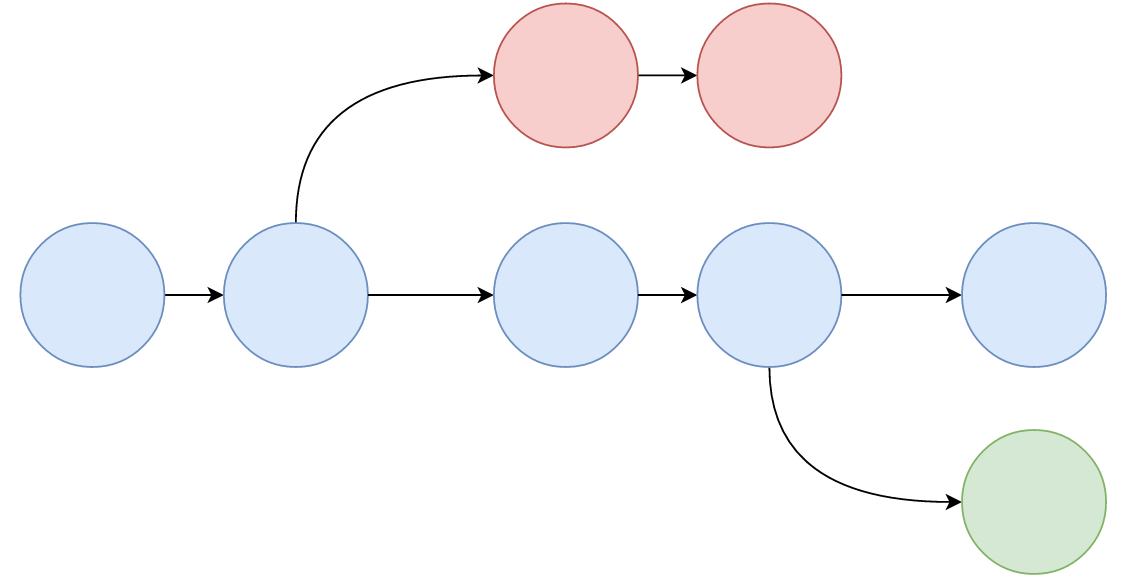
\includegraphics[scale=0.5]{FeatureBranch}
\caption{Primjer tijeka rada grananja funkcionalnosti}
\label{fig:FeatureBranch}
\end{figure}

Tijek rada grananja funkcionalnosti nastoji otkloniti glavni nedostatak centraliziranog tijeka rada - učestalo preplitanje različitih tokova razvoja. Grananje funkcionalnosti također ima jedan glavni i više lokalnih repozitorija. Razlika je u tome što se funkcionalnost implementiraju u grani kreiranoj specifično za nju. Programer za novu funkcionalnost kreira novu granu u lokalnom repozitoriju te u nju dodaje promjene. Po završetku implementacije funkcionalnosti programer granu spaja s glavnom granom centralnog repozitorija. Ovaj proces daje jasniji uvid u napredak projekta i implementirane funkcionalnosti. Isto tako, ovaj proces timu daje priliku revizije obavljenih promjena. Umjesto direktnog spajanja grane moguće je kreirati zahtjev za spajanjem \eng{merge request}. Zahtjev za spajanjem dodatno opisuje promjene ostvarene u sklopu grane te timu daje priliku za komunikaciju i reviziju obavljenih promjena.

\textit{Gitflow} tijek rada također koristi jedan centralni i više lokalnih repozitorija. Za razliku od prijašnja dva tijeka rada, \textit{gitflow} tijek rada povijest repozitorija prati kroz glavnu i razvojnu granu. Razvojna grana \eng{develop branch} vrlo je slična glavnoj grani u procesu grananja funkcionalnosti. Grana za novu funkcionalnost kreira se iz razvojne grane te se pri završetku implementacije u nju spaja. S druge strane, glavna grana sadrži samo produkcijske verzije izvornog koda, odnosno one verzije projekta koje su objavljene korisniku. Kad tim odluči objaviti novu verziju projekta, kreira se nova grana iz trenutnog stanja razvojne grane. Nakon završetka provjere ispravnosti grana se spaja s glavnom i, po potrebi, razvojnom granom. Nova se verzija glavne grane zatim objavljuje. Verzije na glavnoj grani označavaju se s objavljenom verzijom projekta.

Primjer korištenja \textit{gitflow} procesa prikazan je na slici \ref{fig:Gitflow}. Crvenom bojom prikazana je glavna grana, a plavom razvojna grana. Grane funkcionalnosti, prikazane zelenom i žutom bojom granaju se iz razvojne grane te u nju spajaju. Bijelom bojom označena je grana pripreme za objavu nove verzije projekta. Nakon obavljanja pripreme za objavu, grana se spaja s glavnom granom tima, kreirajući novu produkcijsku verziju, te s razvojnom granom kako bi promjene nastale pri pripremi za objavu bile dodane projektu.

\begin{figure}
\centering
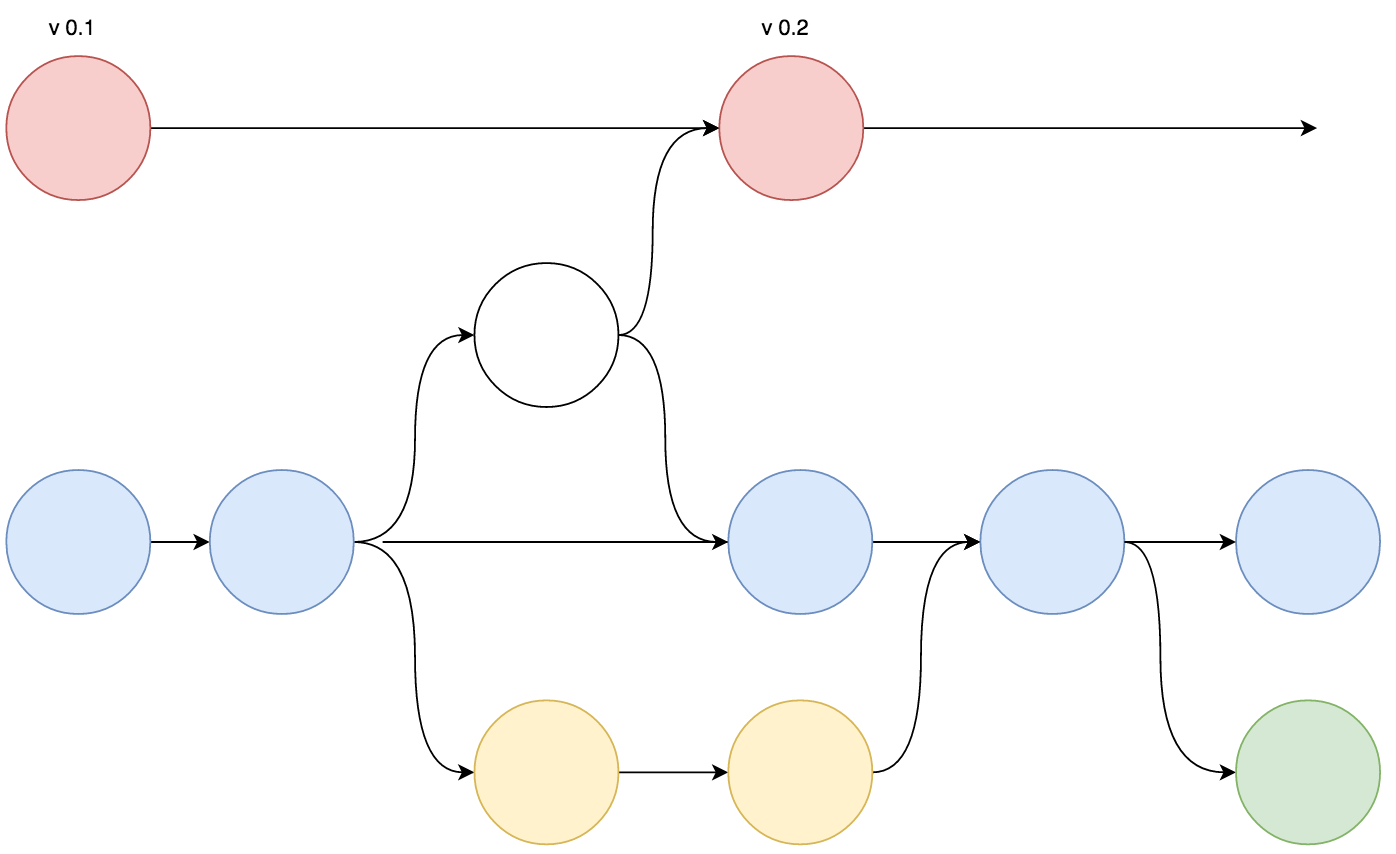
\includegraphics[scale=0.5]{Gitflow}
\caption{Primjer gitflow tijeka rada}
\label{fig:Gitflow}
\end{figure}

Navedeni pristup olakšava upravljanje objave projekta. Buduće da je krucijalno objaviti ispravan produkt, sam proces objave treba biti kontroliran, a produkt temeljito testiran. Izdvajajući proces objave na pomoćnu granu omogućava istovremeno testiranje produkcijske verzije i nastavak rada na novim funkcionalnostima.

Za razliku od ostalih tijekova rada promatranih u ovom poglavlju, forking tijek rada nema centralni repozitorij, već svaki sudionik ima vlastiti javni i privatni repozitorij. Programer vlastiti javni repozitorij kreira kopiranjem drugog javnog repozitorija. Zatim iz vlastitog javnog repozitorija kreira vlastiti privatni repozitorij. Promjene obavlja na privatnom repozitoriju te ih proizvoljno spaja s javnim repozitorijem. Navedene promjene zatim može iskoristiti netko drugi kloniranjem repozitorija ili spajanjem promjena s postojećim repozitorijem. Ujedno, programer može predložiti dodavanje vlastitih promjena drugom repozitoriju. Navedeni se proces naziva zahtjev za povlačenjem promjena \eng{pull request}.

\textit{Forking} tijek rada najčešće se primjenjuje za projekte otvorenog koda. On omogućuje svakom članu zajednice kloniranje, modifikaciju i objavu promjena obavljenih na projektu. Dodatno, zahtjev za spajanje daje vrlo dobar uvid u obavljene promjene bez modifikacije izvornog repozitorija.

Osnova kontinuirane integracije je kontinuirano, odnosno učestalo spajanje radnih kopija s glavnom kopijom. Kad bi se vodio samo ovim principom, centralizirani repozitorij najbolje bi zadovoljavao postavljene zahtjeve. Međutim, centralizirani repozitorij u praksi se ne koristi ni za što osim najjednostavnijih projekata.

Iako drugi tijekovi rada rjeđe obavljaju integraciju radnih kopija, prednosti koje pružaju nadilaze navedeni nedostatak. Također, moguće je smanjiti vrijeme između spajanja radnih kopija. Na primjer, gitflow tijek rada spajanje radne kopije s glavnom kopijom obavlja pri završetku implementacije funkcionalnosti. Što je veća funkcionalnost koja se implementira, to će duže radna kopija ostati izdvojena. Zbog navedenog, posao je potrebno razdijeliti na manje dijelove. To se ne odražava pozitivno samo na proces kontinuirane integracije, već olakšava i praćenje projekta te je sastavni dio agilnog pristupa razvoja programske potpore. Prednosti koje pružaju napredniji pristupi verzioniranju su: lakše praćenje razvoja, zahtjevi za spajanjem i lakša objava projekta u produkciju te nadilaze nešto duže vrijeme izdvojenosti radnih kopija.

U praktičnom dijelu rada koristim \textit{gitflow} tijek rada. Ovaj tijek rada najbolje odgovara zahtjevima i tipu projekta. Isto tako, \textit{gitflow} tijek rada omogućava jednostavniju implementaciju kontinuirane dostave i isporuke. Uz glavnu i radnu granu, repozitoriju ću po potrebi dodavati dodatne grane. Na primjer, isporuku verzija programske potpore za testiranje izdvojit ću u zasebnu granu. Navedeni proces omogućava lako praćenje testnih verzija te olakšava implementaciju procesa isporuke testne verzije.

\paragraph{Verzioniranje u sklopu kontinuirane integracije}

Proces kontinuirane integracije započinje dohvatom željene verzije repozitorija. Kako bi dohvatio željenu verziju, proces kontinuirane integracije mora imati pristup repozitoriju. Xcode Server omogućava korištenje lokalnog ili udaljenog repozitorija verzioniranog svn ili git alatom. Ako se koristi udaljen repozitorij, onda je isti potrebno zaštiti od neželjenog pristupa. Danas se u praksi koriste dva tipa zaštite: HTTPS i SSH autentifikacija.

HTTPS autentifikacija pristup kontrolira korištenjem jedinstvenog korisničkog imena i lozinke. Budući da se proces integracije odvija automatski, potrebno je spremiti i automatizirati unošenje korisničkog imena i lozinke. Preporučeno je iste pohraniti korištenjem Keychain Access aplikacije.

SSH autentifikacija pristup kontrolira korištenjem javnog i privatnog ključa najčešće generiranog korištenjem RSA protokola. Ovaj je tip autentifikacije pogodniji za automatizaciju zbog čega ga koristim u sklopu ovog rada. Proces kreiranja i konfiguriranja SSH autentifikacije detaljnije je objašnjen u sljedećem odlomku.

Xcode Server automatski detektira alat kojim je repozitorij verzioniran. Nakon autentifikacije pristupa je potrebno odabrati granu za koju se kreira proces integracije. Pojedini bot integraciju obavlja za samo jednu granu pa je potrebno kreirati zaseban bot za svaku željenu granu. Slika \ref{fig:BotAddingSSH} prikazuje autentifikaciju detektiranog git repozitorija korištenjem postojećeg SSH ključa.

\begin{figure}
\centering
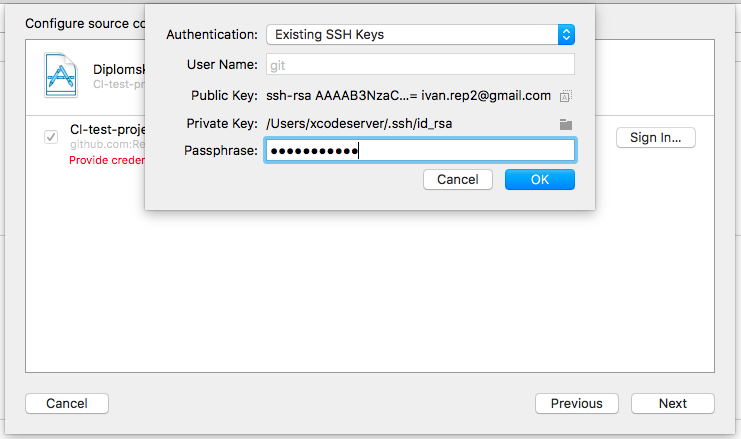
\includegraphics[scale=0.5]{BotAddingSSH}
\caption{Dodavanje SSH ključa}
\label{fig:BotAddingSSH}
\end{figure}

Xcode Server omogućava automatsko pokretanje integracije nakon kreiranja nove verzije na promatranoj grani. Navedenu funkcionalnost Xcode Server ostvaruje kontinuiranom provjerom stanja repozitorija. Proces integracije također je moguće provoditi periodično ili ga pokretati ručno. Slika \ref{fig:CIStartConfig} prikazuje navedene opcije.

\begin{figure}[b!]
\centering
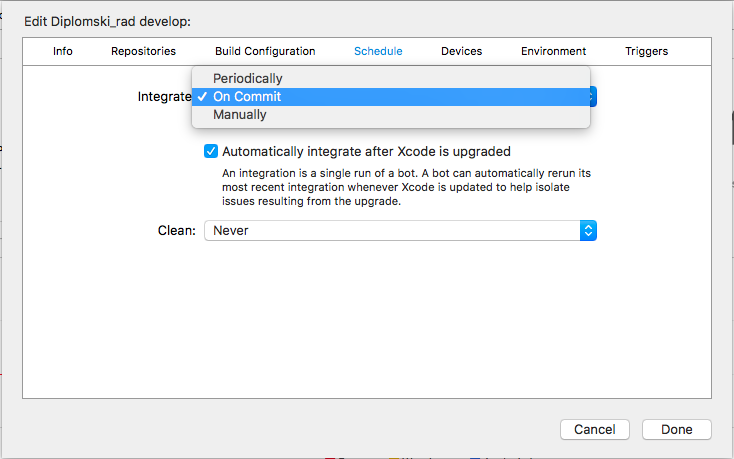
\includegraphics[scale=0.5]{CIStartConfig}
\caption{Odabir načina pokretanja procesa integracije}
\label{fig:CIStartConfig}
\end{figure}

Korištenjem navedenih opcija kontinuirana integracija pokreće se nakon kreiranja novog stanja na odabranoj grani repozitorija.

\paragraph{SSH autentifikacija}

U sklopu rada koristim SSH autentifikaciju za pristup udaljenom git repozitoriju. SSH ključevi obično se pohranjuju u direktoriju \path{~/.ssh}. Ako SSH ključ već ne postoji u navedenom direktoriju, onda ga je potrebno kreirati. Skripta \ref{listing:ssh} prikazuje proces generiranja ključa. Naredba pod \#1 generira novi SSH ključ sa željenom adresom e-pošte. Preporučeno je u tijeku kreiranja ključ zaštititi lozinkom.

Nakon generiranja, ključ je potrebno dodati SSH agentu kako se šifra ključa ne bi morala unositi pri svakom korištenju. Naredbe \#2 i \#3 ostvaruju navedenu funkcionalnost. Na kraju, javni dio ključa potrebno je registrirati na platformi koja \textit{hosta} repozitorij. Naredba \#4 kopira javni dio novokreiranog ključa.

\begin{figure}[b!]
\centering
\includegraphics[scale=0.3]{GitHubSSH}
\caption{Dodavanje SSH ključa na GitHub platformu}
\label{fig:GitHubSSH}
\end{figure}

\begin{lstlisting}[caption=Postavljanje SSH autentifikacije, label=listing:ssh]
ssh-keygen -t rsa -b 4096 -C "{e-mail adresa}" #1

eval "$(ssh-agent -s)" #2

ssh-add -K ~/.ssh/{ime_kljuca} #3

pbcopy < ~/.ssh/{ime_kljuca}.pub #4
\end{lstlisting}

U sklopu rada koristim GitHub platformu. Slika \ref{fig:GitHubSSH} prikazuje proces registriranja SSH ključa na platformi. SSH ključ dodaje se odabirom opcije \textit{Settings -> SSH and GPG keys -> New SSH key} te dodavanjem kopiranog javnog dijela ključa u polje za ključ. Nakon spremanja ključa isti je moguće koristiti za autorizaciju komunikacije s GitHub platformom.

\subsection{Priprema sustava} \label{header:PripremaSustava}

Priprema sustava sastoji se od provjere postojanja, dohvata i konfiguracije potrebnih alata te od pripreme projekta za izgradnju.

Provjeru postojanja alata obavljam korištenjem skripte \ref{listing:PripremaSustavaProvjera}. Naredba \#1 provjerava postojanje alata korištenjem alata \verb|which| koji je dostupan u sklopu instalacije macOS operacijskog sustava. U slučaju nepostojanja alata, potrebno je isti dohvatiti i instalirati.

\begin{lstlisting}[caption=Provjera postojanja alata, label=listing:PripremaSustavaProvjera]
if !(which {ime_alata} >/dev/null); then #1
    {naredba za instalaciju alata} #2
fi
\end{lstlisting}

Na navedeni način provjeravam postojanje i instaliram tri alata, alate za dohvat ovisnosti CocoaPods i Carthage te alat za provjeru ispravnosti koda Swiftlint. Skripta \ref{listing:PripremaSustavaInstalacija} prikazuje automatiziranu instalaciju navedenih alata.


\begin{lstlisting}[caption=Automatizirana instalacija alata, label=listing:PripremaSustavaInstalacija]
if !(which pod >/dev/null); then #1
    echo "Installing CocoaPods"

    gem install cocoapods --user-install
    pod repo update
fi

if !(which carthage >/dev/null); then #2
    echo "Instaling Carthage"

    brew install carthage
fi

if !(which swiftlint >/dev/null); then #3
    echo "Instaling Swiftlint"

    brew install swiftlint
fi
\end{lstlisting}

Naredba pod \#1 provjerava i instalira CocoaPods alat korištenjem alta \verb|gem| dostupnog u sklopu instalacije macOS operacijskog sustava. Kako bih izbjegao unošenje administrativne lozinke, kod instalacije koristim opciju \verb|--user-install| koja alat instalira samo za trenutnog korisnika. Naredbe \#2 i \#3 provjeravaju i instaliraju alate Carthage i Swiftlin korištenjem alata brew.

Konfiguracija Xcode projekta pohranjena je unutar \verb|.xcodeproj| datoteke. Datoteka je namijenjena za modifikaciju i čitanje korištenjem alata Xcode. Datoteka nije pogodna za ručnu izmjenu i čitanje. Za olakšanje nadgledanja i modifikacije postavka projekta se često koriste \verb|xcconfig| datoteke.

Navedene su datoteke tekstualnog formata s \verb|.xcconfig| nastavkom te sadrže listu \verb|{ključ} = {vrijednost}| linija koje specificiraju postavke projekta. Navedene je datoteke potrebno dodati projektu te iskoristiti za konfiguraciju željene sheme. Pomoću Xcode aplikacije je potrebno otvoriti projekt te odabrati željenu shemu i sekciju \verb|Info|. U odjeljku \verb|Configurations| odabirom opcije \verb|Plus| potrebno je kreirati novu konfiguraciju. Slika \ref{fig:XcodeConfigurations} prikazuje proces dodavanja nove konfiguracije.

\begin{figure}[h!]
\centering
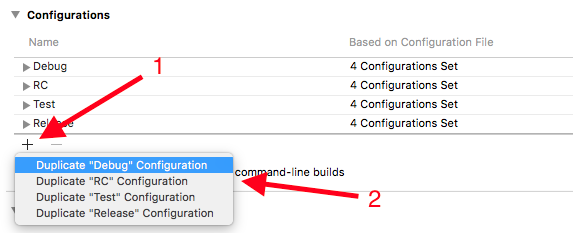
\includegraphics[scale=0.7]{XcodeConfigurations}
\caption{Kreiranje konfiguracije projekta}
\label{fig:XcodeConfigurations}
\end{figure}

\subsection{Upravljanje ovisnostima}

Prije izgradnje projekta potrebno je dohvatiti ovisnosti koje projekt koristi. Za dohvaćanje ovisnosti u iOS razvoju koriste se dva alata: \textit{CocoaPods} i \textit{Carthage}. Oba se sustava široko koriste te izbor uvelike ovisi o osobnom ukusu. Zbog toga u radu koristim oba alata.

\paragraph{CocoaPods}

CocoaPods je stariji, široko prihvaćen, centraliziran alat za upravljanje ovisnostima iOS projekata. Alat je jednostavan i intuitivan za korištenje. Dovoljno je specificirati ovisnosti korištenjem \verb|Podfile| datoteke i pokrenuti proces dohvaćanja ovisnosti. Alat samostalno kreira i konfigurira radno okruženje te time olakšava proces upravljanja ovisnostima.

Međutim, najveći problem alata upravo je ova učestala modifikacija datoteka radnog okruženja. Alat pri svakom dohvatu izmjenjuje postavke izgradnje što može uzrokovati neželjeno ponašanje. Dodatno, budući da je alat centraliziran, sve korištene biblioteke moraju biti registrirane u CocoaPods sustavu. Upravo to otežava korištenje privatnih biblioteka i biblioteka u razvoju.

Inicijalizacija CocoaPods alata je prikazana u skripti \ref{listing:CocoaPodsInit}. Naredbu je potrebno pokrenuti u direktoriju projekta.

\begin{lstlisting}[caption=Inicijalizacija CocoaPods alata, label=listing:CocoaPodsInit]
pod init
\end{lstlisting}

Naredba kreira \verb|Podfile| datoteku koja služi za specifikaciju ovisnosti. Skripta \ref{listing:PodfileExample} prikazuje primjer \verb|Podfile| datoteke. Datoteka za cilj \verb|Diplomski_rad| specificira dvije ovisnosti \verb|LayoutKit| i \verb|Fabric|.

\begin{lstlisting}[caption=Primjer Podfile datoteke, label=listing:PodfileExample]
use_frameworks!

target 'Diplomski_rad' do
    pod 'LayoutKit'
    pod 'Fabric'
end
\end{lstlisting}

Ovisnosti se dohvaćaju pokretanjem naredbe \verb|pod install| u direktoriju projekta.

Skripta \ref{listing:cocoapods} automatizira dohvaćanje ovisnosti korištenjem CocoaPods alata. Naredba \#1 provjerava postojanja Podfile datoteke te u slučaju njezina postojanja nastavlja s izvođenjem skripte. Naredba \#2 provjerava postojanje CocoaPods alata. Ako alat nije instaliran, onda se instalira korištenjem \textit{gem} alata. Na kraju, naredba \#3 dohvaća ovisnosti korištenjem CocoaPods alata.

\begin{lstlisting}[caption=Dohvat ovisnosti korištenjem alata CocoaPods, label=listing:cocoapods]
if [ -f Podfile ]; then #1
    echo "Podfile found. Starting CocoaPods"

    if ! which pod >/dev/null; then #2
        echo "Installing CocoaPods"

        gem install cocoapods --user-install
        pod repo update
    fi

    pod install #3

    echo "Finished dependency fetch using CocoaPods"
fi
\end{lstlisting}

\paragraph{Carthage}

Carthage je noviji, decentralizirani alat za upravljanje ovisnostima. Alat omogućava jednostavno dohvaćanje i izgradnju biblioteke bez potrebe njihove prijašnje registracije. Za razliku od CocoaPods alata, Carthage ne modificira radno okruženje. Ovisnosti je potrebno samostalno uključiti u projekt zbog čega je alat složeniji za korištenje od CocoaPods alata. Međutim, u istom trenutku alat otklanja neželjene posljedice koje nosi učestala izmjena datoteka razvojnog okruženja.

Potrebno je kreirati \verb|Cartfile| datoteku. Datoteka je jednostavna lista ovisnosti zajedno s lokacijom izvornog repozitorija. Skripta \ref{listing:Cartfile} prikazuje primjer \verb|Cartfile| datoteke.

\begin{lstlisting}[caption=Primjer Cartfile datoteke, label=listing:Cartfile]
github "JohnSundell/Unbox"
git "https://gitlab.rep.com/Testni_projekt"
\end{lstlisting}

Primjer dohvaća dvije ovisnosti. Javno javnu ovisnost \verb|Unbox| objavljenu na GitHub platformi te privatnu ovisnost objavljenu na Gitlab platformi.

Dohvaćanje se ovisnosti pokreće naredbom \verb|carthage update|.

Skripta \ref{listing:carthage} implementira dohvaćanje ovisnosti korištenjem Carthage alata. Naredba \#1 provjerava postojanje \verb|Cartfike| datoteke te, u slučaju postojanja iste, nastavlja obavljanje skripte. Naredba \#2 provjerava postojanje Carthage alata te ga dohvaća ako ne postoji. Naredba \#3 dohvaća ovisnosti korištenjem Carthage alata. Za bolje performanse operacije koristim dva argumenta. Argument \verb|--platform ios| specificira dohvaćanje ovisnosti samo za iOS platformu. Argument \verb|--cache-builds| dohvaća ovisnosti samo ako iste nisu već dostupne.

\begin{lstlisting}[caption=Dohvat ovisnosti korištenjem alata Carthage, label=listing:carthage]
if [ -f Cartfile ]; then #1
    echo "Cartfile found. Starting Carthage"

    if !(which carthage >/dev/null); then #2
        echo "Instaling Carthage"

        brew install carthage
    fi

    carthage update --platform ios --cache-builds #3

    echo "Finished dependency fetch using Carthage"
fi
\end{lstlisting}

\paragraph{Automatizacija dohvaćanja ovisnosti}

Obje skripte potrebno je pokrenuti prije obavljanja integracije. Za ostvarenje navedene funkcionalnosti \textit{botu} dodajem skriptu koja se izvršava prije pokretanja integracije \eng{Pre-Integration Script}. Slika \ref{fig:PreIntegrationScript} prikazuje proces dodavanja nove skripte. Skripta se dodaje odabirom opcije \textit{Edit Bot... -> Triggers -> Pre Integration Script}.

\begin{figure}[b!]
\centering
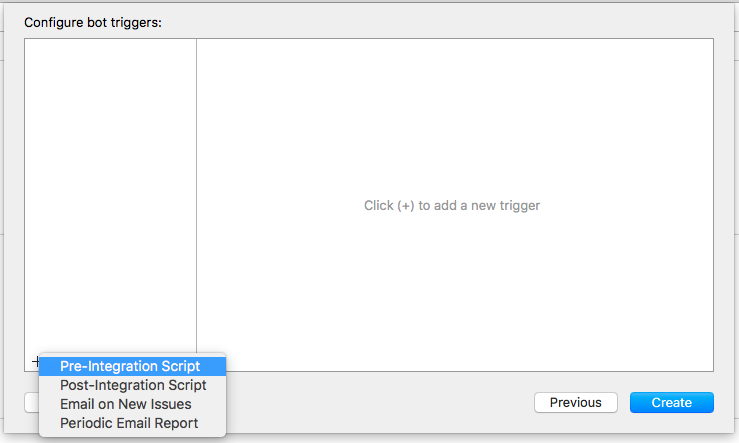
\includegraphics[scale=0.5]{PreIntegrationScript}
\caption{Dodavanje skripte koja se izvršava prije integracije}
\label{fig:PreIntegrationScript}
\end{figure}

Unutar novokreirane skripte potrebno je pozvati sve naredbe koje se trebaju izvršiti prije integracije. Radi jednostavnosti i fleksibilnosti navedene je naredbe korisno izdvojiti u zasebnu datoteku. Korištenjem ovog pristupa olakšavam implementaciju kontinuirane integracije te omogućavam laku izmjenu skripte koja se izvršava prije integracije. Skripta \ref{listing:pre_integration_script_call} se korištenjem \path{XCS_PRIMARY_REPO_DIR} varijable okruženja navigira u početni direktorij projekta te provjerava postojanje datoteke \path{scripts/preintegration}. U slučaju postojanja datoteke ista se izvršava.

\begin{lstlisting}[caption=Poziv skripte koja se izvršava prije obavljanja integracije, label=listing:pre_integration_script_call]
#!/bin/bash

cd $XCS_PRIMARY_REPO_DIR

if [ -f scripts/preintegration ]; then
    ./scripts/preintegration
fi
\end{lstlisting}

Skripta \ref{listing:pre_integration_script} se izvršava prije integracija. Skripta jednostavno poziva prethodno definirane skripte. Na isti je način moguće dodati proizvoljan broj naredbi. Također, skripta u \textit{PATH} varijablu okruženja dodaje dvije putanje koje olakšavaju korištenje postojećih alata.

\begin{lstlisting}[caption=Skripta koja se izvršava prije integracije, label=listing:pre_integration_script]
#!/bin/bash

export PATH="/usr/local/bin:~/.gem/ruby/2.0.0/bin/:$PATH"

if [ -f scripts/cocoapods ]; then
    ./scripts/cocoapods
fi

if [ -f scripts/carthage ]; then
    ./scripts/carthage
fi
\end{lstlisting}

Sve se skripte trebaju nalaziti u \path{scripts} direktoriju repozitorija.

\subsection{Izgradnja}

Izgradnja iOS aplikacija obavlja se korištenjem alata \textit{xcodebuild}\citep{xcodebuild}. Razvio ga je Apple za izgradnju programske potpore za macOS operacijski sustav. Alat je vrlo moćan te pruža veliki broj funkcionalnosti i mogućih konfiguracija. S vremenom je i proširen te danas podržava izgradnju aplikacija za iOS, tvOS i watchOS operacijske sustave. Alat izgradnju obavlja korištenjem Xcode projekta. Prije definiranja procesa izgradnje potrebno je upoznati se sa strukturom Xcode projekta.

Xcode je službeni Appleov alat za razvoj programske potpore za iOS i macOS operacijske sustave. Na tržištu postoji nekoliko alternativa, ali Xcode daleko je najkorišteniji. Svi alati koriste alat xocdebuild za izgradnju te zbog toga imaju vrlo sličnu strukturu projekta. Ovaj tip projekta naziva se Xcode projekt.

Xcode projekt sadrži jedan ili više ciljeva \eng{target} i jednu ili više shema \eng{scheme}. Cilj definira postavke koje se koriste kod izvršavanja operacije za navedeni cilj. Jedan projekt može sadržavati više ciljeva. Pomoću ciljeva moguće je isti kod distribuirati za različite verzije operacijskog sustava, različite operacijske sustave i testirati projekt. Shema definira koji se cilj koristi za koju operaciju. Projekt može koristiti više shema kako bi objedinio operacije za pojedinu distribuciju. Odnos cilja i sheme prikazan je na slici \ref{fig:TargetScheme}. Projekt sadrži tri cilja i dvije sheme. Sheme različito definiraju koji se cilj koristi za koju operaciju.

\begin{figure}[b!]
\centering
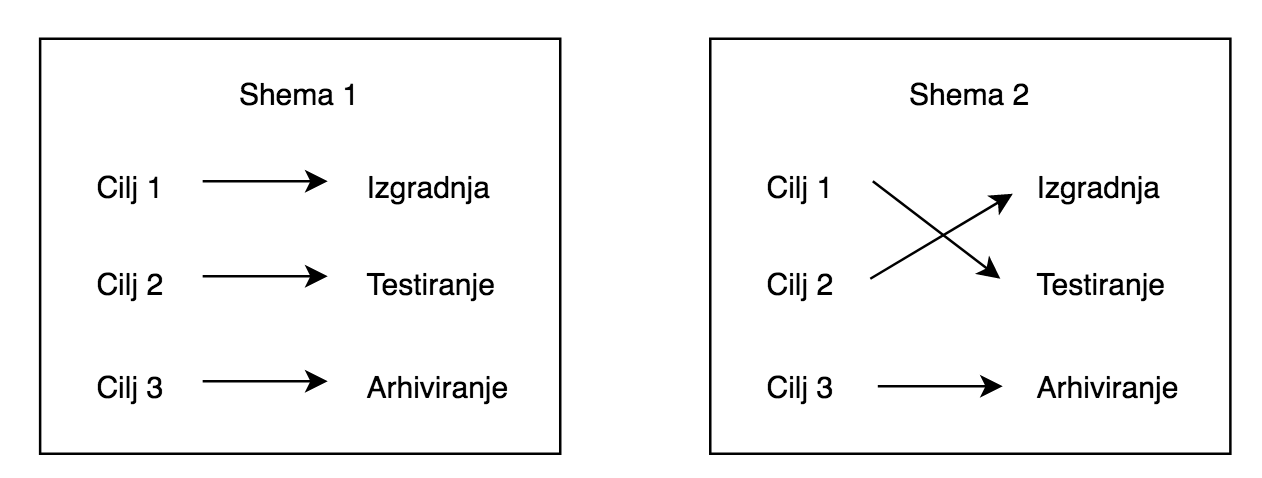
\includegraphics[scale=0.5]{TargetScheme}
\caption{Xcode projekt s tri cilja i dvije sheme}
\label{fig:TargetScheme}
\end{figure}

Xcode projekte moguće je grupirati u Xcode radno okruženje \eng{workspace}. Radno okruženje olakšava segmentiranje velikog projekta i olakšava upravljanje ovisnostima.

Izgradnja iOS projekta u praksi se pokreće gotovo isključivo korištenjem alata Xcode. Međutim, navedeni pristup nije moguće automatizirati. Zbog navedenog, procesi koji automatiziraju izgradnju koriste alat xcodebuild direktno ili koriste alat koji interno koristi xcodebuild. Alat je detaljnije specificiran u dodatku \ref{header:xcodebuild}.

\begin{figure}
\centering
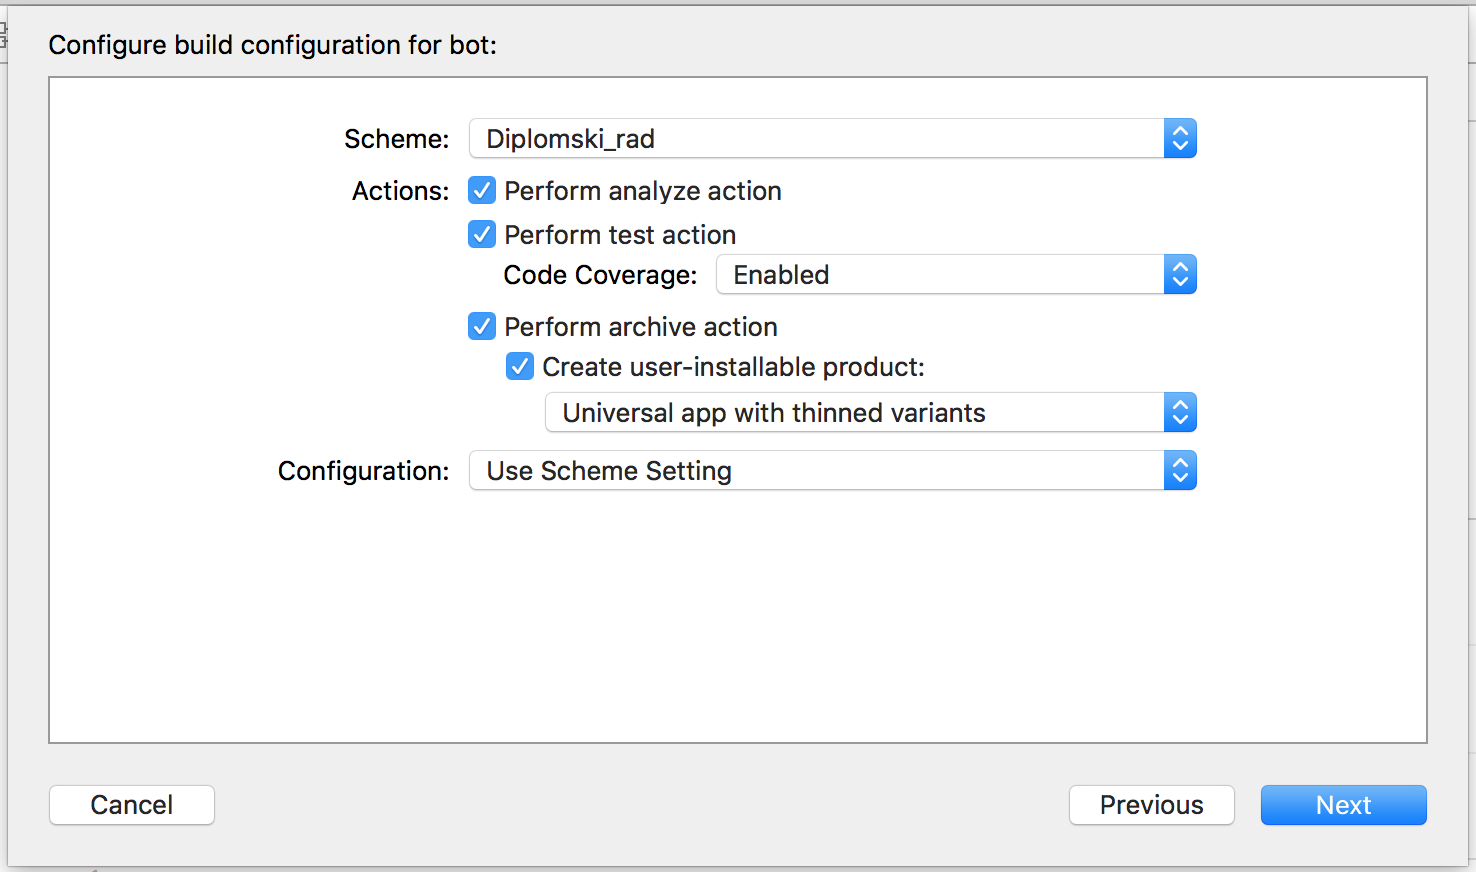
\includegraphics[scale=0.5]{XcodeServerOptions}
\caption{Konfiguracija osnovnih opcija integracije}
\label{fig:XcodeServerOptions}
\end{figure}

\begin{figure}[b!]
\centering
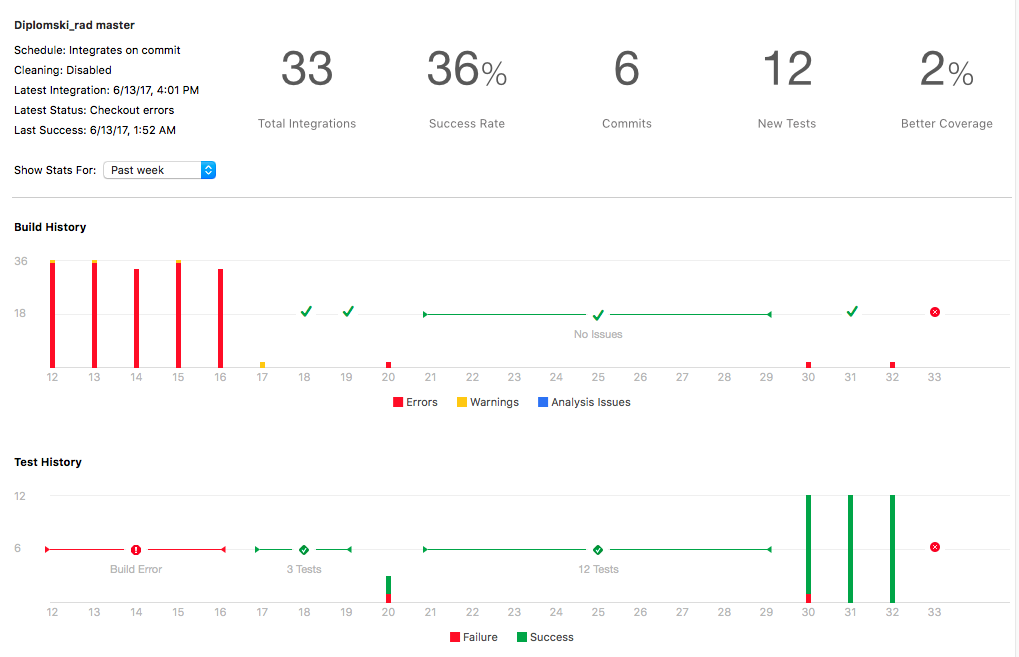
\includegraphics[scale=0.5]{XcodeServerResult}
\caption{Primjer prikaza rezultata kontinuirane integracije}
\label{fig:XcodeServerResult}
\end{figure}

Xcode Server značajno olakšava korištenje alata xcodebuild. Nakon povezivanja \textit{bota} s repozitorijem izvornog koda, moguće je konfigurirati opcije integracije. Moguće je i odabrati shemu projekta za koju se provodi integracija, operacije koje će se izvršavati u sklopu integracije te postavke koje se koriste za izgradnju projekta. Slika \ref{fig:XcodeServerOptions} prikazuje opcije koje se mogu konfigurirati.

Kako bi se shema mogla iskoristiti za integraciju, ona mora biti javno objavljena. Shema se može konfigurirati korištenjem Xcode aplikacije.

Ovako konfiguriran \textit{bot} provodi kontinuiranu integraciju za odabranu granu. Rezultat integracije moguće je vidjeti otvaranjem početnog ekranu \textit{bota}. Slika \ref{fig:XcodeServerResult} prikazuje primjer rezultata integracije. Prvi redak slike prikazuje opće informacije o kontinuiranoj integraciji kao što su broj obavljenih integracija, postotak uspješnosti te broj verzija repozitorija. Drugi redak slike prikazuje uspješnost izvođenja procesa izgradnje za svaku pojedinu integraciju.

Prve dvije prikazane integracije završile su greškom koja je u trećoj integraciji otklonjena. Četvrta integracije otklanja upozorenje dojavljeno u prve tri integracije. Integracija broj 20 dojavljuje novu grešku koju otklanja sljedeća integracija.

Odabirom pojedine integracije otvara se ekran s detaljima odabrane integracije. Detalji integracije podijeljeni su u nekoliko sekcija od kojih svaka pruža vrlo detaljne informacije o integraciji. Prva sekcija \verb|Summary| prikazuje najvažnije podatke na jednom, sažetom ekranu. Slika \ref{fig:XcodeServerSingleIntegration} prikazuje primjer navedene sekcije za integraciju koja je dojavila pet novih pogrešaka u procesu izgradnje. Detalji novopronađenih pogrešaka prikazani su na ekranu što olakšava pronalaženje i otklanjanje pogrešaka.

\begin{figure}
\centering
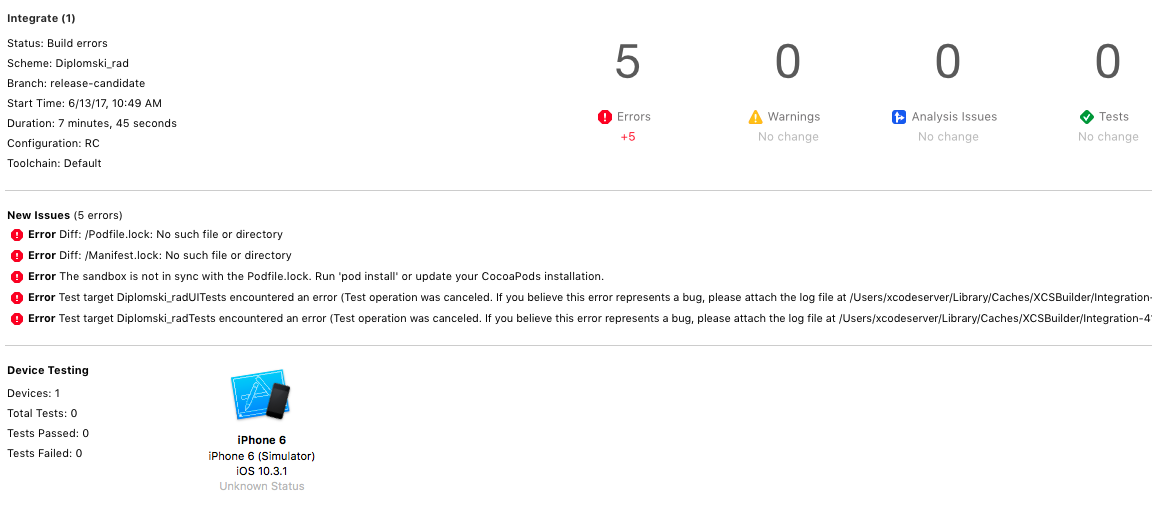
\includegraphics[scale=0.4]{XcodeServerSingleIntegration}
\caption{Detaljan prikaz integracije}
\label{fig:XcodeServerSingleIntegration}
\end{figure}

Zadnja sekcija detaljnog prikaza integracije prikazuje ispis svih faza integracije, uključujući i ručno definirane faze. Sekcija je vrlo korisna za provjeru ponašanja pojedine faze.

\section{Testiranje}

Testiranje je sastavni dio razvoja programske potpore. Implementacijom kvalitetnih testova ne samo da se osigurava ispravan rad programske potpore, već se i spriječava nazadovanje koda \eng{code regression} te značajno smanjuje potreba za ručnim testiranjem ispravnosti\citep{wiki:SoftwareTesting}.

Pogrešno je mišljenje da implementacija testova produljuje vrijeme razvoja. Svaku implementiranu funkcionalnost i obavljenu izmjenu potrebno je testirati. Jedino je pitanje hoće li se navedeno testiranje obavljati automatski. Jednom napisan kvalitetan test može se pokrenuti proizvoljan broj puta. S druge strane, provođenje ručnog testiranja svaki put zahtijeva vrijeme članova tima. Bilo to u sklopu razvoja ili s ciljem provjere ispravnosti, ručna provjera ispravnosti zahtijeva više resursa i daje lošije rezultate.

Navedenu konstataciju ne treba zamijeniti s potpunim isključenjem ručnog testiranja aplikacije. Bez obzira na kvalitetu testova, pogreške se uvijek mogu dogoditi. Međutim, pisanjem kvalitetnih testova vjerojatnost pojave pogreške značajno se smanjuje.

Ovaj odlomak ne ulazi u proces pisanja testova, već samo automatizira njihovo pokretanje. Implementacija kvalitetnih testova vrlo je složeno područje te nadilazi okvire ovog rada.

Proces razvoja programske potpore za iOS operacijski sustav definira dva tipa testova: \textit{unit} i \textit{UI} testove.

\textit{Unit} testovi su nesretno imenovani. Oni ne predstavljaju standardne \textit{unit} testove, već se koriste kao ime za testove koji imaju pristup kodu koji testiraju. Testovi direktno komuniciraju s kodom koji testiraju i putem ove komunikacije provjeravaju ispravnost izvođenja. Ovaj tip testa pokreće se kao omotač oko izvorne aplikacije.

S druge strane, \textit{UI} testovi nemaju pristup izvornom kodu aplikacije. Oni programsku potporu testiraju njezinim pokretanjem i simuliranjem korisničke interakcije. Programer specificira korisničke akcije i ponašanje koje očekuje od aplikacije nakon primanja navede akcije. \textit{UI} testovi pokreću dvije aplikacije: aplikaciju koju testiraju i aplikaciju koja simulira korisničku interakciju.

Oba tipa testova implementirani su kao testni ciljevi Xcode projekta. Kod testnog cilja je odvojen te se ne koristi u procesu izgradnje. Testni cilj referencira cilj koji testira. Dodatno, shema može specificirati koji se testni ciljevi pokreću prilikom pokretanja operacije testiranja. Na ovaj način jedna shema može u procesu testiranja pokrenuti više testnih ciljeva.

Proces testiranja može se pokrenuti na iOS Simulatoru, aplikaciji koja simulira iOS operacijski sustav na macOS operacijskom sustavu, ili na stvarnom uređaju. Simulator se instalira u sklopu instalacije Xcode aplikacije.

\subsection{Automatizacija testiranja}

\begin{figure}[b!]
\centering
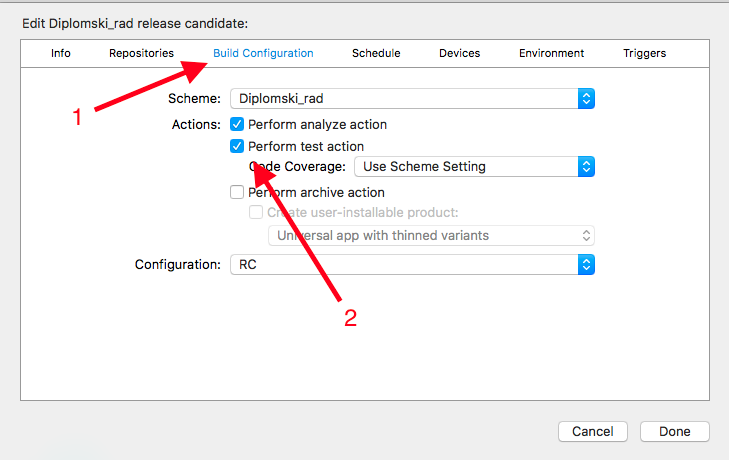
\includegraphics[scale=0.5]{XcodeServerTestAction}
\caption{Uključivanje pokretanja testova u sklopu integracije}
\label{fig:XcodeServerTestAction}
\end{figure}

\begin{figure}
\centering
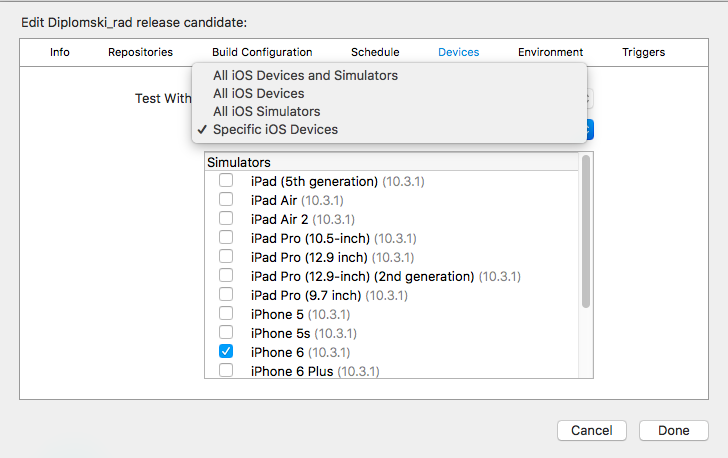
\includegraphics[scale=0.5]{XcodeServerTestDevices}
\caption{Odabir uređaja na kojima se pokreću testovi}
\label{fig:XcodeServerTestDevices}
\end{figure}

Xcode Server detektira testne ciljeve sheme za koju obavlja proces integracije. Za pokretanje testova u sklopu integracije treba odabrati opciju \verb|Edit bot...| te u sekciji \verb|Build configuration| označiti opciju \verb|Perform test action|. Slika \ref{fig:XcodeServerTestAction} prikazuje navedeni proces. Sljedeća obavljena integracija pokrenut će sve testne ciljeve koje definira odabrana shema.

Isto tako, moguće je odabrati uređaje na kojima se pokreću testovi. Testove je moguće pokrenuti na svim dostupnim uređajima, samo na dostupnim iOS simulatorima, samo na dostupnim stvarnim uređajima ili na samo odabranim uređajima. Slika \ref{fig:XcodeServerTestDevices} prikazuje navedeni izbornik. Izborniku se pristupa odabirom opcije \verb|Edit bot...| te otvaranjem sekcije \verb|Devices|.

Novi se testni cilj shemi može dodati korištenjem Xcode aplikacije. Treba pokrenuti iOS projekt te odabrati željenu shemu iz padajućeg izbornika u gornjoj alatnoj traci aplikacije. Odabirom opcije \verb|Edit scheme| otvara se prozor prikazan na slici. U lijevom izborniku treba odabrati opciju \verb|Test| te pritiskom na plus ikonu dodati željeni testni cilj postojećoj shemi. Nakon spremanja promjene integracija u sljedećem izvršavanju obavlja i novododani testni cilj.

\begin{figure}[b!]
\centering
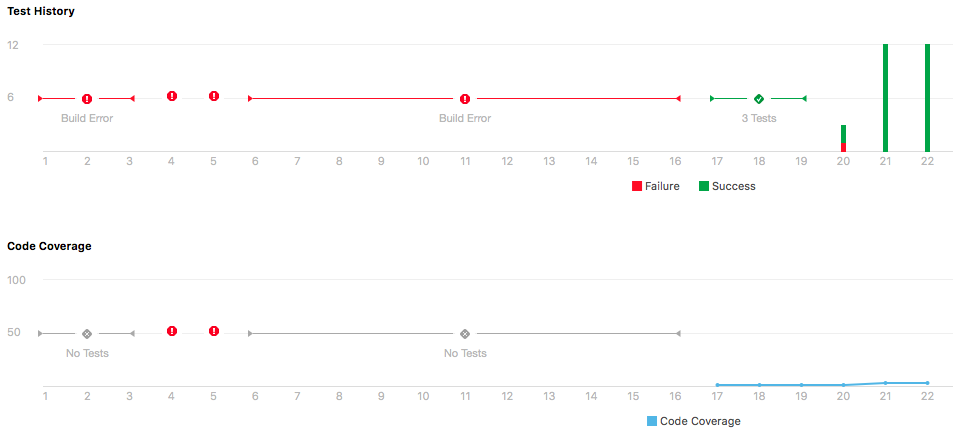
\includegraphics[scale=0.4]{XcodeServerTestResult}
\caption{Rezultati procesa testiranja i osiguranja kvalitete}
\label{fig:XcodeServerTestResult}
\end{figure}

Rezultati obavljanja testova također su prikazani na početnom ekranu \textit{bota} u sekciji \verb|Test History|. Osim broja uspješnih i neuspješnih testova, alat omogućuje i prikaz detaljnih rezultata testiranja. Odabirom rezultata testiranja pojedine integracije prikazuju se detalji odabranog testiranja.


\section{Osiguranje kvalitete}

Osiguranje kvalitete \eng{code quality} proces je u sklopu programskog inženjerstva koje postavljanjem umjetnih restrikcija nastoji poboljšati kvalitetu koda i konačnog produkta. Restrikcije se najčešće definiraju u obliku pravila koja moraju biti zadovoljena. Pravila se mogu kretati od jednostavnih do vrlo složenih te uvelike ovise o korištenim alatima i potrebama tima.

U sklopu rada implementiram dvije provjere: provjeru pokrivenosti koda testovima i provjeru ispravnosti koda korištenjem alata Swiftlint.

Pokrivenost koda testovima \eng{code coverage} mjera je koja govori u kojem je postotku izvorni kod pokriven testovima. Svaki redak koda koji je barem jednom izvršen u procesu testiranja pokriven je testovima. Što je navedena mjera veća to je više koda testirano. Zbog toga se može reći da veća pokrivenost koda testovima, u generalnom slučaju, vodi do bolje kvalitete konačnog produkta.

Međutim, navedena se mjera može vrlo lako zloupotrijebiti. Na primjer, moguće je napisati vrlo jednostavan test koji samo pokreće aplikaciju i time poziva značajan postotak koda. Zbog navedenog se u praksi često koriste modificirane verzije mjerenja pokrivenosti koda testovima koje procesu dodaju dodatna pravila te time nastoje utvrditi stvarnu kvalitetu testiranja\citep{wiki:CodeCoverage}.

Alat xcodebuild implementira mjerenje pokrivenosti koda testovima. Dovoljno je naredbi za pokretanje testova dodati argument \verb|-showBuildSettings|. Ispis naredbe pohranjuje se kao skup datoteka koje služe za vizualan prikaz pokrivenosti koda testovima u Xcode aplikaciji. Uz sam postotak pokrivenosti koda testovima, Xcode prikazuje i pokrivenost pojedinog dokumenta te broj poziva svake pojedine linije koda.

Xcode Server također pruža navedenu opciju, ali u reduciranom obliku. Prikupljanje podataka o pokrivenosti koda testovima uključuje se odabirom opcije \path{Code Coverage -> Enabled} u postavkama bota. Slično Xcode aplikaciji, Xcode Server uz postotak pokrivenosti koda testovima prikazuje i pokrivenost pojedinog dokumenta. Slika \ref{fig:XcodeServerTestCoverage} prikazuje pokrivenost datoteka testnog projekta testovima.

\begin{figure}[h!]
\centering
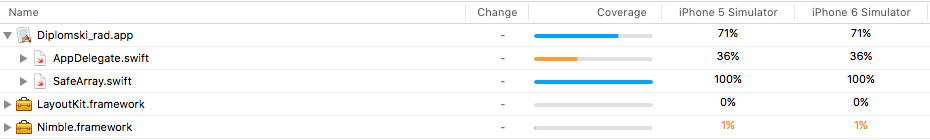
\includegraphics[scale=0.45]{XcodeServerTestCoverage}
\caption{Pokrivenost datoteka testnog projekta testovima}
\label{fig:XcodeServerTestCoverage}
\end{figure}

Swiftlint je alat za statičku analizu koda napisanog u programskom jeziku Swift. Alat definira veliki broj pravila kojima nastoji osigurati praćenje stila i konvencija jezika Swift\citep{SwiftLint}. Većina pravila se odnosi na izgled i format koda, ali postoje i pravila koja nastoje izbjeći pojavu grešaka. Slični alati su kreirani za gotovo svaki programski jezik koji se koristi u praksi. Ovi alati se nazivaju alati za uređivanje koda \eng{linting tools}. Navedene alate uglavnom kreira i održava zajednica.

Ne poštivanje pravila izaziva dojavu upozorenja \eng{warning} ili greške \eng{error}. Moguće je kreirati nova pravila i modificirati ili isključiti postojeća. Veliki broj timova definira vlastiti stil pisanja koda koji je moguće osigurati korištenjem navedenih funkcionalnosti.

Alati za uređivanje koda postaju nezaobilazni u praksi. Pridržavanje strogog formata pisanja koda olakšava timski rad, poboljšava čitljivost koda i izbjegava pojavu lako izbjegnutih grešaka.

Alat se pokreće pozivom naredbe \path{swiftlint} u početnom direktoriju projekta. Naredbu je moguće ukljućiti u proces izgradnje korištenjem \verb|Run Script| faze. Pomoću Xcode aplikacije otvoriti željeni projekt te odabrati cilj koji izvršava izgradnju. U sekciji \verb|Build Phases| odabirom opcije \verb|Plus -> New Run Script Faze| kreirati novu fazu. Fazi dodati sadržaj skripte \ref{listing:swiftlint}.

\begin{lstlisting}[caption=Provjera postojanja i pokretanje Swiftlint alata, label=listing:swiftlint]
if which swiftlint >/dev/null; then
    swiftlint
else
    echo "warning: Swiftlint nije instaliran"
fi
\end{lstlisting}

Ako je poziv \path{swiftlint} naredbe dodan kao faza izgradnje, onda se naredba obavlja prilikom svake izgradnje. Ispis naredbe se parsira zajedno s ispisom xcodebuild alata te se rezultati dojavljuju zajedno. Ako naredba nije dodana projektu onda je poziv potrebno ručno implementirati nakon obavljanja integracije.


\chapter{Kontinuirana dostava} \label{header:KontinuiranaDostava}

Kontinuirana dostava je praksa u sklopu programskog inženjerstva koja automatiziranjem procesa isporuke programske podrške nastoji olaškati i time povećati učestalost isporuke produkta u produkciju. Proces isporuke može biti kompleksan i vremenski zahtjevan. Prije isporuke je produkt potrebno izgraditi, testitirati, kreirati artefakt koji se isporučuje te ga objaviti na željenoj platformi. Za izgradnju je potrebno dohvatiti željenu verziju repozitorija, pripremiti sustav te dohvatiti sve potrebne ovisnosti.

Navedeni proces je vremenski zahtjevan zbog čega se on ne provodi često. Rijetko provođenje procesa isporuke uzrokuje nekoliko problema. Prvo, rijetkom isporukom se veći broj funkcionalnosti grupira i isporučuje zajedno. Što je veći broj funkcionalnosti isporučen zajedno i što duže te funkcionalnosti nisu isporučene, to je teže osigurati ispravnost isporučenih funkcionalnosti. Dodatno, što duže funkcionalnost nije objavljena to je veći propušteni dobitak koji je funkcionalnost mogla donjeti. Svaka funkcionalnost se razvija s određenim ciljem. Nakon što je funkcionalnost razvijena a prije nego što je objavljena navedeni cilj ostaje bespotrebno ne ispunjen.

Automatizacija procesa isporuke značajno olakšava navedeni proces i time potiče češću isporuku. Dodatno, implementacija jednostavnog i automatiziranog procesa isporuke smanjuje mogućnost pojave ljudske pogreške. Kontinuirana dostava na navedeni naćin nastoji smanjiti trošak, rizik i vrijeme razvoja programske potpore te isto vrijeme poboljšati kvalitetu i osigurati ispravnost programskog produkta\citep{wiki:ContinuousDelivery}.

Kao što je navedeno u uvodu poglavlja, programsku potporu je prije isporuke potrebno izgraditi, testirati te kreirati artefakt za isporuku. Iako različiti razvojni procesi različito nazivaju artefakt za distribuciju, zbog konzistentnosti ga nazivam arhiva. Arhiviranje je proces kreiranje arhive programske potpore. Arhiva omogućava instalaciju programske potpore na operacijskom sustavu za kojeg je programska potpora izgrađena.

Jednako tako je prije automatizacije isporuke produkta potrebno automatizirati izgradnju, testiranje, provjeru ispravnosti i arhiviranje programske potpore. Proces automatizacije izgradnje, testiranja i provjere ispravnosti se naziva kontinuirana integracija te je definiran u poglavlju \ref{header:Kontinuirana_Integracija}. Kontinuirana dostava obuhvaća proces kontinuirane integracije te proces automatizacije isporuke.

Međutim, u praksi se pojam kontinuirana dostava češće koristi za proces automatizacije isporuke koji zahtijeva odvojenu implementaciju procesa kontinuirane integracije. Zbog jednostavnosti se navedeni pristup koristi u ovom radu. Proces izgradnje, testiranja i provjere ispravnosti implementiram u sklopu kontinuirane integracije na koju dodajem automatizaciju isporuke i time ostvarujem kontinuiranu dostavu.

Važno je napomenuti da kontinuirana dostava ne isporučuje produkt automatski, već samo automatizira proces isporuke. Tim još uvijek mora pokrenuti proces isporuke za željenu verziju produkta. Automatska objava programske potpore je obrađena u sljedećem, \ref{header:KontinuiranaIsporuka} poglavlju.

Programsku potporu je moguće isporučiti na više načina - direktnom instalacijom na mobilni uređaj, ručnom distribucijom arhive, objavom arhiva korištenjem distribucijske platforme ili objavom arhive koriptenjem App Store platforme. Navedeni tipovi isporuke dijele sličan proces izgradnje i arhiviranja ali se značajno razlikuju u procesu objave arhive. Samim time se i automatizacije navedenih načina isporuke značajno razlikuju.

iOS operacijski sustav podržava četiri tipa isporuke: direktnu isporuku \eng{direct distribution}, \textit{ad hoc} isporuku \eng{ad hoc distribution}, unutarnju isporuku \eng{in-house distribution} i isporuku korištenjem App Store platforme. Odabir načina isporuke ovisi o korisnicima za koje se obavlja isporuka.

Direktna isporuka progrmsku potporu instalira direktno na povezani mobilni uređaj. Mobilni uređaj mora biti povezan s računalom koje obavlja isporuku te mora biti registriran kao testni uređaj na Apple Developer platformi. Ovaj tip isporuke programsku potporu instalira na jedan uređaj koji mora biti direktno povezan s računalom zbog čega se koristi gotovo isključivo u sklopu razvoja i za isporuku programske potpore unutar razvojnog tima. Dodatno, ovaj se tip isporuke se nemože niti bi ga bilo pogodno automatizirati. Zbog sigurnosnih razloga Apple nije objavio proces direktne isporuke već ju je moguće obaviti isključivo korištenjem Xcode aplikacije.

Ad hoc i unutarnja isporuka su vrlo slične. Obje proizvode arhivu koju je potrebno samostalno dostaviti željenim korisnicima. Arhiva se može dostaviti ručno, na primjer korištenjem e-mail poruke ili se može objaviti na platformi za distribuciju programske potpore. Moguće je kreirati vlastitu platformu ili iskoristiti neku velikog broja već postojećih. Isporuke se razlikuju u tome što uređaji na koje se instalira programska potpora isporučena ad hoc načinom isporuke moraju biti registrirani kao testni uređaju na Apple Developer platformi dok to nije potrebno za unutanju isporuku. Zbog navedenog je korištenjem unutranje isporuke programsku potporu moguće isporučiti neograničenom broju korisnika. Za korištenje unutarnje isporuke je potrebno posjedovati \textit{Enterprise} Apple Developer račun, skuplju verziju običnog Apple Developer računa.

Ad hoc isporuka se najčešće koristi za isporuku programske potpore unutar tima, na primjer za isporuku testne verzije aplikacije timu za osiguranje kvalitete. Unutarnja isporuka se koristi gotovo isključivo za isporuku aplikacija razvijenih za unutarnje potrebe kompanije. Ovaj tip isporuke se nesmije iskoristiti za objavu aplikacija namijenjenih za javno tržište.

App Store isporuka se koristi za objavu programske potpore namijenjene za javno tržište. Za razliku od ostalih tipova isporuke, Apple strogo nadzire aplikacije objavljene ovim tipom isporuke. Svaka aplikacija koja zatraži objavu prolazi kroz strog proces provjere kvalitete i podudaranja s velikim brojem Appleovih smjernica. Ovaj proces može trajati i nekoliko tjedana zbog čega je nužno osigurati ispravnost aplikacije prije pokretanja procesa. Svaka izmjena aplikacije prolazi nešto kroz kraći proces provjere koji može trajati od nekoliko sati do nekoliko dana.

Iako se navedeni tipovi isporuke razlikuju u implementaciji, moguće ih je generalno podijeliti u tri ista koraka: potpisivanja koda, arhiviranja programske potpore i objave arhive. Svaki od koraka je definiran i automatiziran odvojeno u nastavku poglavlja. Slika \ref{fig:ContinuousDelivery} prikazuje navedenu podjelu.

\begin{figure}
\centering
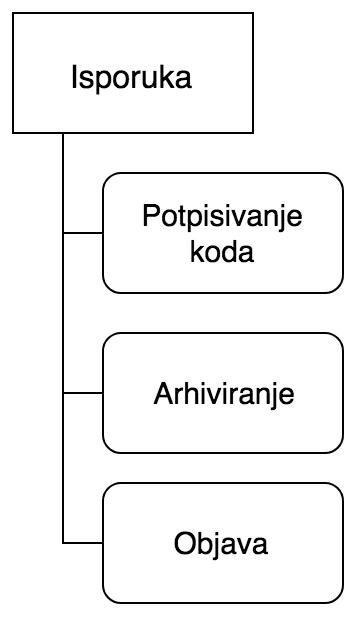
\includegraphics[scale=0.6]{ContinuousDelivery}
\caption{Proces isporuke}
\label{fig:ContinuousDelivery}
\end{figure}

\section{Potpisivanje koda} \label{header:PotpisivanjeKoda}

Kako bi osigurao autentičnost i neizmjenjenost programske potpore, iOS operacijski sustav implementira proces potpisivanja koda \eng{code signing}. Proces korištenjem certifikata, identifikatora aplikacije \eng{application identificator} i pripremnih profila \eng{provisioning profiles} potpisuje i enkriptira kreiranu arhivu. Prije kreiranja arhive je potrebno kreirati i dohvatiti navedene artefakte te ispravno konfigurirati proces arhiviranja.

Proces postpisivanja koda se može podijeliti na tri faze: kreiranje artefakata, dohvat artefakata i konfiguracija procesa arhiviranja. Slika \ref{fig:CodeSigning} prikazuje navedenu podjelu.

\begin{figure}
\centering
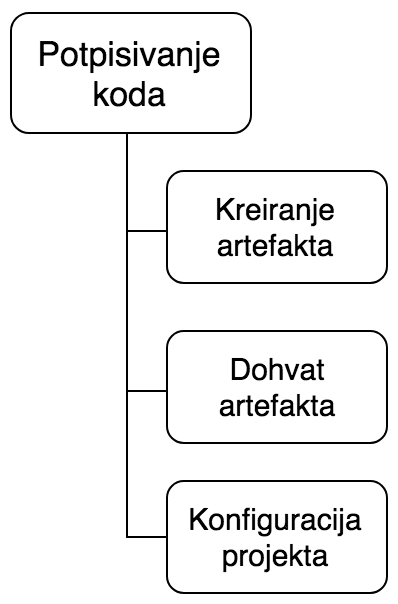
\includegraphics[scale=0.6]{CodeSigning}
\caption{Potpisivanje koda}
\label{fig:CodeSigning}
\end{figure}

Ako potrebni artefakti ne postoje iste je potrebno kreirati te nakon toga preuzeti i instalirati na računalu. Proces arhiviranja je zatim potrebno konfigurirati kako bi koristio ispravne artefakte.

Svi artefakti se kreiraju i dohvaćaju korištenjem \path|https://developer.apple.com| platforme. Potrebno se je prijaviti na platformu korištenjem Apple Developer računa, odabrati opciju \verb|Certificates, Identifiers & Profiles| i željeni tip artefakta iz lijevog bočnog izbornika.

Certifikati se koriste za osiguranje nekoliko različitih procesa zbog čega postoji nekoliko tipova certifikata. U sklopu isporuke nas zanimaju dva tipa certifikata: razvojni \eng{development} i produkcijski \eng{production} certifikati. Razvojni certifikati se koriste u razvoju i za direktnu isporuku programske potpore. Uobičajno je kreirati zaseban certifikat za svakog člana tima. Produkcijski certifikati se koriste za ad hoc, unutarnju i App Store isporuku. Standardno je kreirati jedan certifikat po timu koji obavlja isporuku. Certifikat se kreira pomoću \verb|CSR| datoteke koju je moguće kreirati korištenjem Keychain Access aplikacije.

Pokrenuti Keychain Access aplikaciju te u izborniku na vrhu ekrana odabrati opciju \verb|Certificate Assistant -> Request a Certificate|. U novo otvorenom prozoru unijeti e-mail adresu Apple Developer računa, odabrati \verb|Save to disk| opciju i lokaciju spremanja novo kreirane datoteke. Kreiranu datoteku dostaviti u formu za kreiranje certifikate na Apple Developer platformi te nakon toga obrisati datoteku.

Za korištenje certifikata je potrebno posjedovati certifikat i privatni ključ kojim je on kreiran. Certifikat je moguće preuzeti s Apple Developer platforme dok je privatni ključ potrebno dohvatiti s računala koje posjeduje privatan ključ. Nakon kreiranja certifikata to je isključivo uređaj koji je kreirao CSR datoteku. Za dohvat privatnog ključa pokrenuti Keychain Access aplikaciju te pronaći željeni certifikat. Ako na uređaju postoji privatni ključ navedenog certifikata, isti je moguće izdvojiti korištenjem opcije \textit{Export}. Slika \ref{fig:PrivateKeyExport} prikazuje izdvajanje privatnog ključa certifikata.

\begin{figure}
\centering
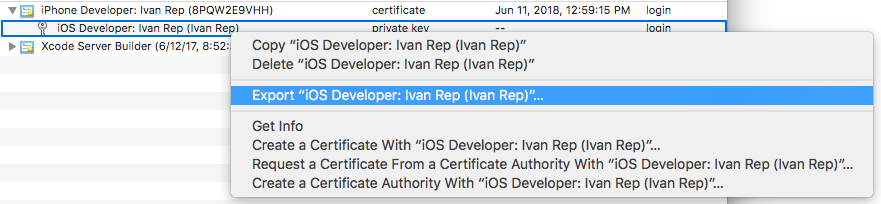
\includegraphics[scale=0.47]{PrivateKeyExport}
\caption{Izdvajanje privatnog ključa certifikata}
\label{fig:PrivateKeyExport}
\end{figure}

Ovako izdvojeni privatni ključ certifikata je moguće distribuirati. Nužno je osigurati tajnost privatnog ključa jer suprotno narušava sigurnost svih aplikacija koje koriste navedeni certifikat.

Identifikator aplikacije identificira i opisuje servise koje koristi aplikacija koja se isporučuje. Identifikator aplikacije je definiran pomoću identifikatora paketa \eng{bundle identifier}, niza znakova jedinstvenog za svaku aplikaciju. Identifikator paketa je najčešće oblika \path{com.ime_kompanije.ime_aplikacije}. Postoje dva tipa identifikatora aplikacije: \textit{wildcard} i eksplicitni identifikatori aplikacije. Wildcard identifikatori aplikacije specificiraju samo dio identifikatora paketa te ih karakterizira asterisk (*) u sklopu imena, na primjer \path{com.rep.*}. Sve aplikacije čiji identifikator paketa započinje navedenim nizom znakova mogu biti isporućene korištenjem navedenog identifikatora. Wildcard identifikatori se koriste u razvoju programske potpore. Eksplicitni identifikatori jedinstveno identificiraju aplikaciju, na primjer \path{com.rep.testna_aplikacija} te se koriste za isporuku specifične aplikacije.

Za kreiranja identifikatra aplikacija je potrebno specificirati ime identifikatora, dodati identifikator paketa i odabrati servise koje aplikacija koristi. Nakon kreiranja je identifikator potrebno preuzeti i pokrenuti korištenjem Keychain Access aplikacije.

Pripremni profil povezuje identifikator aplikacije i certifikat. Svaki od četiri tipa isporuke definira vlastiti tip pripremnog profila. Kreiranje pripremnog profila započinje odabirom tipa profila i odabirom odgovarajućeg identifikatora aplikacije i certifikata. Pripremni profil za direktnu isporuku zahtijeva razvojni certifikat, dok pripremni profili ostalih tipova isporuka zahtijevaju produkcijski certifikat.

\begin{figure}
\centering
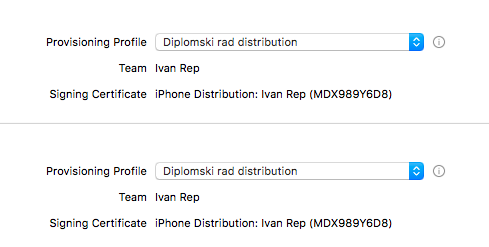
\includegraphics[scale=0.6]{SigningArtefactsSetup}
\caption{Postavljanje artefakta za potpisivanje koda}
\label{fig:SigningArtefactsSetup}
\end{figure}

Novo kreirana artefakte je potrebno preuzeti i pripremiti za korištenje. Profile je potrebno spremiti na računalu koje obavlja isporuku u direktoriju \path|~/Library/MobileDevice/Provisioning Profiles/| a certifikate je potrebno pokrenuti korištenjem Keychain Access aplikacije.

Prije pokretanja arhiviranja je potrebno konfigurirati projekt kako bi se u sklopu arhiviranja koristili ispravni artefakti. Otvoriti Xcode projekt, odabrati željen cilj u sekciji \textit{General} podstaviti \textit{Debug} i \textit{Release} certifikate za potpisivanje koda.

\begin{figure}[b!]
\centering
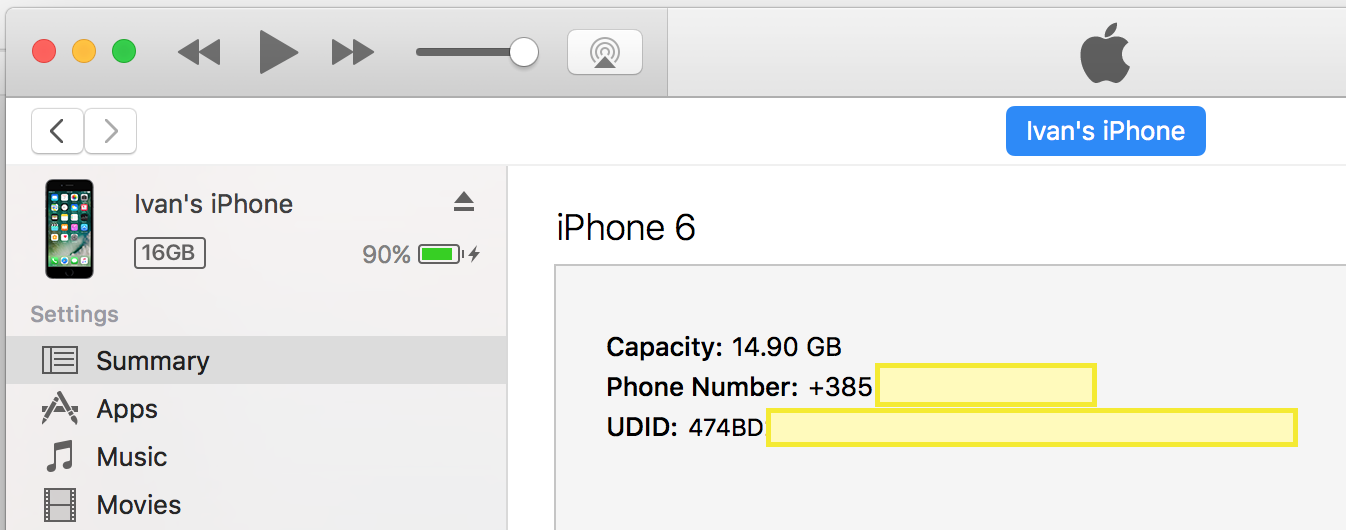
\includegraphics[scale=0.5]{iTunesUUID}
\caption{Dohvat UUIDa uređaja korištenjem iTunes aplikacije}
\label{fig:iTunesUUID}
\end{figure}

Direktna i ad hoc isporuka zahtijevaju registraciju mobilnog uređaja kao testnog uređaja korištenjem Apple Developer platforme. Uređaj se registrira korištenjem njegovog UUID identifikatora. UUID se može dohvatiti korištenjem iTunes aplikacije dostupne u sklopu instalacije macOS operacijskom sustavu. Potrebno je povezati mobilni uređaj s računalom korištenjem USB kabela te u iTunes aplikaciji odabrati povezani mobilni uređaj i kopirati njegov UUID. Slika \ref{fig:iTunesUUID} prikazuje lokaciju UUID broja u iTunes aplikacije.

\subsection{Automatizacija potpisivanja koda} \label{header:AutomatizacijaPotpisivanjaKoda}

Ručno kreiranje i održavanje certifikati i profila se može vrlo lako zakomplicirati. Ne samo da je proces kreiranja sam po sebi složen, već je potrebno i ispravno distribuirati artefakte bez ugrožavanja njihove sigurnosti. Artefakte se mogu slobodno distribuirati, ali je njihove privatne ključeve nužno održati tajnim. Do prije nekoliko godina se je cijeli proces odrađivao ručno. Nakon kreiranja artefakata isti su se zajedno s privatnim ključem pohranili na sigurnu lokaciju te distribuirali po potrebi.

Danas na tržištu postoji nekoliko pristupa i alata koji olakšavaju i automatiziraju proces potpisivanja koda. Automatizacija potpisivanja koda se oslanjaju na javan API Apple Developer platforme koji omogućuje kreiranje, modificiranje i dohvat svih artefakata navedenih u prošlom odlomku.

Dodatno, večina alata se zalaže za pohranu artefakata zajedno s pripadajučim privatnim ključevima u jednom tajnom git repozitoriju. Na ovaj se način njihova pohrana i dohvat značajno pojednostavljuju te je cijeli proces moguće jednostavno automatizirati. Međutim, pohrana sigurnosnih podataka u git repozitoriju donosi i određeni sigurnosni rizik. Pristup repozitoriju je nužno detaljno nadzirati. Preporuća se SSH protokol definirana u \ref{header:Verzioniranje} odlomku. Dodatno, korisno je repozitorij pokrenuti unutar lokalne mreže kako on ne bi bio vidljiv izvan mreže\citep{codesigningguide}.

Automatizaciju potpisivanja koda u ovom radu ostvarujem korištenjem alata \verb|match| koji je dio \verb|fastlane| familije\citep{fastlane:match}. Alat samostalno kreira, dohvaća i priprema potrebne artefakte i time značajno olakšava proces potpisivanja koda.

Alat match se inicijalizira pozivanjem naredbe \verb|fastlane match init| u početnom direktoriju projekta. Proces inicijalizacije zahtijeva unos lokacije git repozitorija te autorizaciju pristupa repoztoriju. Lokacija repozitorija se zajedno s ostalim parametrima alata sprema u \verb|Matchfile| datoteku gdje je iste moguće modificirati..

Match radi povećanja sigurnosti zahtjeva da SSH ključ korišten u procesu SSH autentifikacije bude vidljiv samo trenutnom korisniku operacijskog sustava. Skripta \ref{listing:ssh_chmod} modificira prava pristupa za odabrani ključ kako bi njegovo korištenje bilo dostupno samo trenutnom korisničkom računu operacijskog sustava.

\begin{lstlisting}[caption=Ograničavanje prava pristupa SSH ključu na samo trenutnog korisnika, label=listing:ssh_chmod]
chmod 600 ~/.ssh/{imekljuca}.pub
\end{lstlisting}

Dodatno, potrebno je konfigurirati SSH protokol kako bi isti koristi željeni ključ. Kreirati novu datoteku \path|.ssh/config| sa sadržajem skripte \ref{listing:SSH_match}.

\begin{lstlisting}[caption=Postavke SSH protokola za alat match, label=listing:SSH_match]
Host *
UseKeychain yes
AddKeysToAgent yes
IdentityFile ~/.ssh/{imekljuca}
\end{lstlisting}

Alata match sve potrebne certifikate i profile kreira i dohvaća automatski. Dovoljno je pokrenuti alat i specificirati tip isporuke koji se koristi. Alat definira četiri tipa koji odgovaraju prethodno definiranim tipovima isporuke: \verb|development|, \verb|adhoc|, \verb|enterprise| i \verb|appstore|. Naredba u nastavku dohvaća i po potrebi kreira artefakte za ad hoc isporuku.

\begin{lstlisting}[caption=Dohvćanje artefakta pomoću dodatka match za ad hoc isporuku]
match(type: 'adhoc')
\end{lstlisting}

Alat ne obavlja konfiguraciju procesa arhiviranja, međutim, budući da je istu potrebno napraviti samo jednom ona se najčešće obavlja ručno. Pomoću match alata kreirati sve potrebne artefakte odnosno pozvati match naredbe za svaki tip isporuke koja se koristi. Navedene će naredbe kreirati i dohvatiti potrebne artefakte. Zatim otvoriti Xcode aplikaciju i odabrati željenu shemu. Na početnoj, \verb|General| sekciji sheme u odlomku \verb|Signing| za svaku konfiguraciju postaviti odgovarajući pripremni profil.

Nakon spremanja promjena se cijeli proces potpisivanja koda svodi na poziv alata match sa željenim tipom isporuke.


\section{Arhiviranje} \label{header:RucnaIsporuka}

Arhiviranje je proces kreiranja artefakta pomoću kojeg se aplikacija instalira na korisničkom uređaju. Artefakt se naziva arhiva aplikacije te je označena \verb|.ipa| nastavkom. Za instalaciju aplikacije je uz arhivu potrebna i datoteka koja opisuje, verificira i locira arhivu. Navedena se datoteka naziva manifest te je označena \verb|.plist| nastavkom.

Proces arhiviranja se za ad hoc, unutarnju isporuku i App Store ispruku razlikuje jedino u odabiru tipa isporuke. Arhiviranje obavlja alat xcodebuild. Međutim, alat je vrlo složen i pruža veliki broj opcija zbog čega na tržištu postoji nekoliko alata koji olakšavanju njegovo korištenje. U sklopu rada za ručno arhiviranje koristim aplikaciju Xcode a za automatizirano arhiviranje alat fastlane odnosno njegov dodatak \verb|gym|. Proces arhiviranja korištenjem alata xcodebuild je prikazan u dodatku \ref{header:xcodebuild}.

Korištenjem aplikacije Xcode odabrati opciju \verb|Product -> Archive| iz izbornika na vrhu ekrana. Nakon kračeg perioda se otvara novi prozor koji prikazuje sve dosad kreirane arhive. Jedino što je potrebno je arhivu izdvojiti za objavu. U prozoru odabrati opciju \verb|Export...|. Otvara se novi prozor u kojem je potrebno odabrati željeni tip isporuke te odabrati između nekoliko opcija kreiranja arhive. Slika \ref{fig:XcodeArchiveOptions} prikazuje početni ekran prozora odnosno odabir tipa isporuke arhive. Nakon odabira željene opcije slijediti upute za dovršenje izdvajanja arhive.

\begin{figure}
\centering
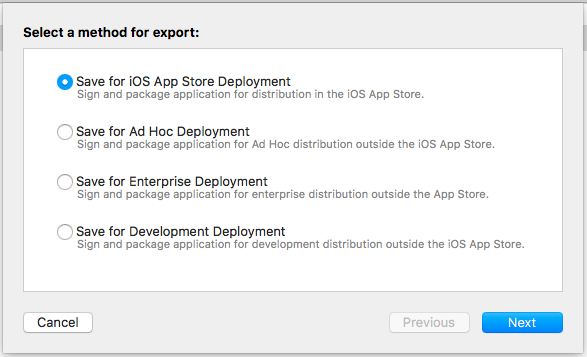
\includegraphics[scale=0.6]{XcodeArchiveOptions}
\caption{Odabir tipa isporuke u procesu kreiranja arhive}
\label{fig:XcodeArchiveOptions}
\end{figure}

Proces generira dvije datoteke prethodno definirane datoteke. Arhivu aplikacije s \verb|.ipa| nastavkom i manifest aplikacije s \verb|.plist| nastavkom.

Direktna isporuka aplikaciju instalira na mobilni uređaj koji je direktno povezan s računalom koje obavlja isporuku. Zbog navedenog proces arhiviranja u sklopu direktne isporuke ne rezultira arhivom već istu direktno instalira na uređaj. Dodatno, ovaj tip arhiviranja je moguće ostvariti isključivo korištenjem Xcode aplikacije. Apple zbog sigurnosnih razloga ne želi objaviti proces direktne instalacije aplikacije na uređaj. Arhiviranje i instalacija se obavlja odabirom željenog povezanog mobilnog uređaja i pokretanjem \verb|run| operacije na željenoj shemi.

\subsection{Automatizacija arhiviranja}

Xcode Server implementira funkcionalnost arhiviranja aplikacije u sklopu obavljanja integracije. Međutim, funkcionalnost je vrlo ograničena. Nije moguće dinamički konfigurirati artefakte koji se koriste za potpisivanje koda niti podesiti argumente arhiviranja.

Zbog navedenog automatizaciju arhiviranja ostvarujem korištenjem fastlane dodatak \verb|gym|. Alat za izgradnju interno koristi alat xcodebuild i na prvi pogled se od njega ne razlikuje značajno. Međutim, ako se za cijeli proces isporuke koristi \verb|fastlane| familija, onda korištenje alata \verb|gym| značajno olakšava implementaciju.

Alat izgrađuje i arhivira aplikaciju te omogućava vrlo jednostavnu konfiguraciju oba procesa. Dodatno, alat automatski detektira i koristi artefakte za potpisivanje koda dohvaćene korištenjem dodatka match. Skripta \ref{listing:gym_archive} prikazuje arhiviranje projekta za ad hoc tip isporuke.

\begin{lstlisting}[caption=Arhiviranje aplikacije za ad hoc isporuku pomoću dodatka gym, label=listing:gym_archive]
gym(scheme: "Diplomski_rad", export_method: "ad-hoc")
\end{lstlisting}

Kreiranje arhive pomoću xcodebuild alata se ostvaruje pozivanjem naredbe uz korištenje opcije \verb|archive|. Shema i time cilj na temelju kojeg se izgrađuje arhiva se definira jedna kao i kod drugih opcija naredbe \verb|xcodebuild|.


\section{Objava}

Za dovršetak isporuke je željenim korisnicima potrebno omogućiti instalaciju aplikacije korištenjem kreirane arhive. Navedeni se proces naziva objava programske potpore. Isporuka programske potpore korištenjem App Store platforme arhivu naravno objavljuje na App Store platformi. S druge strane, ad hoc i unutarnja isporuka arhivu mogu objaviti na nekoliko načina.

Kako bi pokrenuo instalaciju ili osvježenje verzije aplikacije, korisnik mora preuzeti ispravno konfigurirani manifest. Manifest uz podatke o aplikaciji sadrži i lokaciju arhive. Nakon preuzimanja manifesta operacijski sustav samostalno pokreće dohvat arhive i instalaciju aplikacije.

Najjednostavniji ali i najograničeniji način objave je manifest i arhivu objaviti na generalnoj platformi za dijeljne podataka kao što su Dropbox i Goole Drive. Navedene platforme omogućavaju kreiranje URIa za pojedinu datoteke. Potrebno je kreirati URI za objavljenu arhivu i istu dodati manifestu. Iako je ovaj način isporuke na prvi pogled jednostavan, on je vremenski vrlo zahtjevan. Svaku novu verziju je potrebno ručno dodati na platformu, konfigurirati te zatim obavijestiti korisnike o novoj verziji.

Za objavu je moguće kreirati vlastitu platformu. Na primjer, jednostavnu HTML stranicu koja omogućava preuzimanje manifesta koji referencira arhivu obavljenu na vlastitom poslužitelju. Međutim, na tržištu postoji nekoliko platformi koje već implementiraju navedenu funkcionalnost. U sklopu rada promatram dvije platforme ovog tipa, \textit{Mobile Device Management} i \textit{Crashlytics} platforme.

Za objavu programskog produkta za iOS operacijski sustav je moguće koristi službeni Appleov alat \textit{Mobile Device Management, MDM}. Alat je namijenjen za jednostavnu isporuku i distribuciji aplikacija koje nisu namijenjene za javnu objavu. Po funkcionalnosti koje pruža je platforma vrlo sličan App Store platformi. MDM omogućava jednostavnu objavu aplikacije i kontrolu pristupa te omogućava automatsku izgradnju i osvježenje verzije aplikacije. Međutim, alat je skup te nije popularan u zajednici.

\subsection{Crashlytics}

Crashlytics je trenutno najpopularnija od svih platformi za objavu programske potpore za iOS operacijski sustav. Platforma je jednostavna, besplatna te omogućava automatizaciju procesa isporuke. Navedenu platformu koristim u ovom radu. Razvoj platforme je započet 2011. godine. Platforma je osnovana s ciljem jednostavnog praćenja i dojave pogreška pri izvršavanju mobilnih aplikacija. Kompaniju je 2013. godine kupio Twitter a početkom 2017. godine preuzeo Google. Danas alat uz praćenje pogrešaka olakšava distribuciju aplikacija i pračenje velikog broja metrika.

Prije implementacije isporuke je potrebno kreirati profil aplikacije na platformi. Kreiranje profila odrađuje Crashlytics biblioteka koju je potrebno dodati i pokrenuti zajedno s aplikacijom.

Prvo, dodati ovisnosti definirane u skripti \ref{listing:crashlytics} u \verb|Podfile| datoteku.

\begin{lstlisting}[caption=Ovisnosti potrebne za objavu korištenjem Crashlytisc platforme, label=listing:crashlytics]
pod 'Fabric'
pod 'Crashlytics'
\end{lstlisting}

Nakon toga kreirati novu \verb|Run scrip| fazu za željeni cilj te joj dodati skriptu \ref{listing:fabric_run_script}.

\begin{lstlisting}[caption=Fabric Run Script faza, label=listing:fabric_run_script]
"${PODS_ROOT}/Fabric/run" {api_kljuc} {tajni_kljuc}
\end{lstlisting}

API i tajni ključ je potrebno dohvatiti korištenjem Fabric platforme. Otvoriti poveznicu \path{https://www.fabric.io/settings/organizations}. Nakon prijave odabrati željenu organizaciju te preuzeti ključeve.

Na kraju, dodati naredbu \verb|Fabric.with([Crashlytics.self])| na početak \verb|application(application: didFinishLaunchingWithOptions:)| metode klase \verb|AppDelegate|. Registracija aplikacije će se dogoditi prilikom prvog pokretanja aplikacije. Profil aplikacije se nakon pokretanja aplikacije nalazi na stranici \path|https://fabric.io/home|.

Nakon kreiranja profila je arhivu i manifest moguće ručno dodati na Crashlytics platformu.

\paragraph{Automatizacije objave}

Za automatizacije objave korištenjem Crashlytics platforme koristim fastlane dodatak \verb|crashlytics|. Dodatak omogućava jednostavnu objavu aplikacije uz minimalnu konfiguraciju projekta te se nadovezuje direktno na dodatak gym. Za pokretanje dostavje je potrebno pokrenuti naredbu nakon arhiviranja projekta. Skripta \ref{listing:crashlytics_deploy} prikazuje fastlane stazu koja izgrađuje, arhivira i objavljuje aplikaciju na Crashlytics platformi.

\begin{lstlisting}[caption=Fastlane staza za isporuku korištenjem Crashlytics platforme, label=listing:crashlytics_deploy]
lane :develop do
    increment_build_number

    match(app_identifier: "com.rep.Diplomski-rad.development", type: "development")
    gym(scheme: "Diplomski_rad", export_method: "development")

    crashlytics(
        api_token: {api_kljuc},
        build_secret: {tajni_kljuc},
        groups: 'Rep'
    )

end
\end{lstlisting}

Dodatno, kako prilikom pokretanja naredbe ne bi morao unositi crashlytics API i tajni ključ, iste je moguće specificirati kao argumente crashlytics naredbe. Grupa testera kojoj će aplikacija biti vidljiva se može dodati kao argument Crashlytics naredbi - \verb|groups: {ime_grupe}|.

\subsection{App Store}

Objava javnih iOS aplikacija se ostvaruje korištenjem App Store platforme. App Store je službena platforma za distribuciju programske potpore za macOS, iOS, tvOS i watchOS operacijske sustave. Uz dostupnost aplikacije svim korisnicima navedenih operacijskih sustava, platforma pruža i brojne druge funkcionalnosti kao što su automatsko instaliranje novih verzija aplikacija i praćenje ponašanja korisnika.

Objava programske potpore na App Store platformu se obavlja korištenjem iTunes Connect web stranice. iTunes Connect omogućava kreiranje, modificiranje i praćenje objavljene programske potpore. Prije objave je potrebno kreirati profil aplikacije korištenjem iTunes Connect alata.

Kreiranje profila se obavlja na \path|https://itunesconnect.apple.com/| stranici. Nakon prijave je potrebno odabrati opciju \verb|My Apps| te kreirati novi profil. Slika \ref{fig:iTunesConnectAppCreation} prikazuje formu za kreiranje profila aplikacije.

\begin{figure}[b!]
\centering
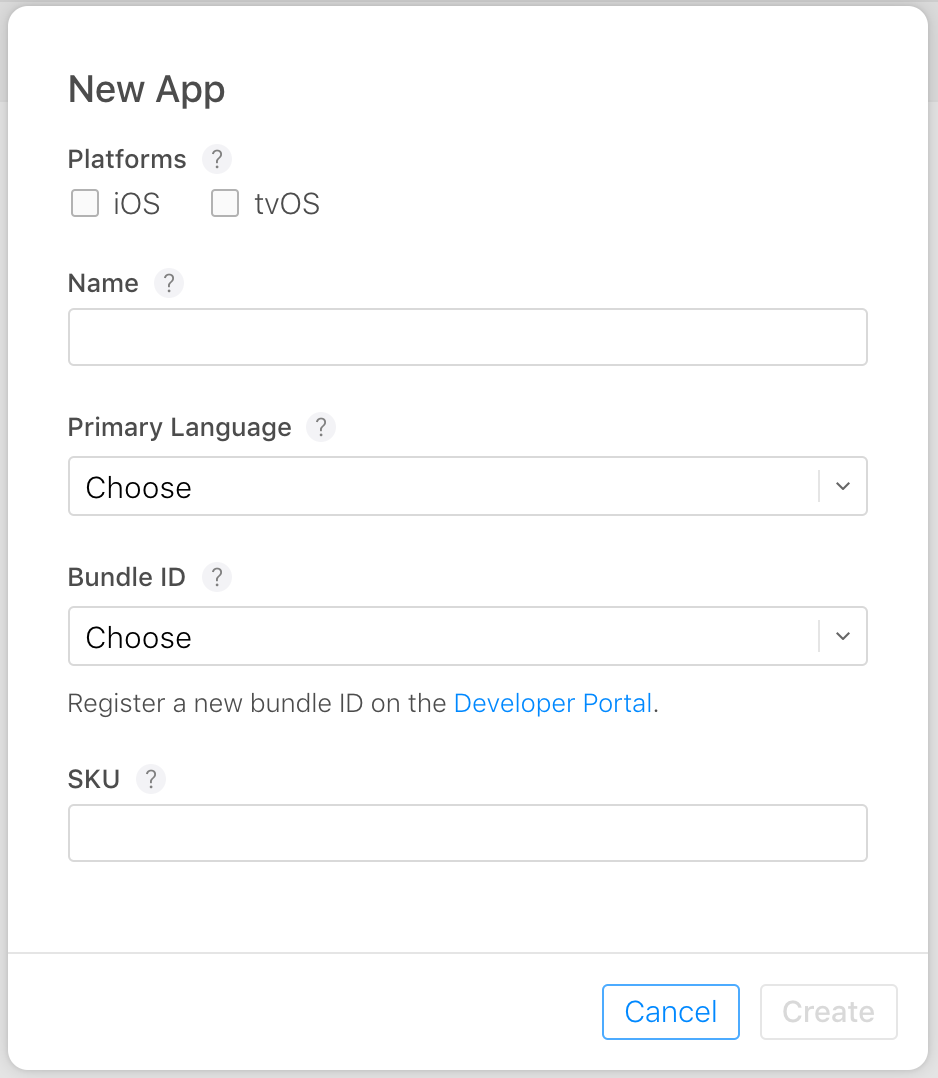
\includegraphics[scale=0.4]{iTunesConnectAppCreation}
\caption{Forma za kreiranje profila aplikacije na iTunes Connect web stranici}
\label{fig:iTunesConnectAppCreation}
\end{figure}

Nakon kreiranja profila aplikacije je potrebno ispuniti dodatne podatke o aplikaciji kao što su opis i kategorija aplikacije. Slično kao i kod Crashlytics platforme, sada je moguće jednostavno dostaviti arhivu i manifest aplikacije.

Iako isporuka aplikacija korištenjem App Store platforme donosi brojne prednosti, ona donosi i brojne nedostatke. Ovaj tip isporuke je poprilično složen te traje puno duže u usporedbi s ostalim tipovima isporuke. Apple vrlo strogo regulira aplikacije koje se nalaze na App Store platformi.

Proces provjere aplikacije zna trajati i do nekoliko tjedana te često rezultira odbijanjem aplikacije. Aplikacija može biti odbijena jer je previše slična već postojećoj aplikacije, jer se ne slaže s nekom od Appleovih politika, zbog loše implementacije i brojnih drugih razloga. Nakon otklanjanja razloga odbijanja je potrebno ponovno proći cijeli proces.

Za objavu nove verzije aplikacije je potrebno proći nešto blažu provjeru. Ona može trajati od nekoliko sati do nekoliko dana te najčešće završava odobrenjem promjena. Odbijanje promjena je vrlo rijetko te služi prvenstveno za prevenciju očitog narušavanja Appleovih politika.

Ovaj proces isporuke je složen i dugotrajan. Iako se u zadnjih nekoliko godina proces značajno poboljšao, veliki broj članova industrije je još uvijek vrlo nezadovoljan. Međutim, Apple zabranjuje isporuku aplikacija za javnu uporabu korištenjem bilo koje druge metode. Ako navedeni proces usporedimo s procesom isporuke web aplikacija, onda su njegovi nedostaci jasno vidljivi. Nova verzija web aplikacije se isporučuje jednostavno promjenom verzije koja se nalazi na poslužitelju. Prvi sljedeći korisnik koji pristupi služitelju automatski koristi sljedeću verziju. Ne samo da je proces isporuke iOS aplikacija daleko teži i sporiji, već korisnik mora samostalno preuzeti novu verziju aplikacije.

Apple nastoji što jednostavnije i neprimjetnije osvježiti verzije aplikacije. Aplikacije se automatski osvježuju kad je uređaj spojen na WiFi mrežu te je dovoljno napunjen. Međutim, određeni broj korisnika isključuje ovu funkcionalnost ili ručno odobrava svaku novu verziju aplikacije. Zbog navedenog uvijek postoji određeni postotak korisnika koji vrlo dugo koriste starije verzije aplikacije. Navedeno iziskuje dugoročnu podršku starijih verzija aplikacije što značajno otežava razvoj.

Zbog navedenih razloga prominenti pojedinci u iOS zajednici predviđaju skoru zamjenu App Store platforme nekim boljim načinom isporuke. Međutim, Apple nije objavio nikakvu naznaku ovog te smo za sad ograničeni sustavom koji imamo.

\paragraph{Automatizacija objave}

Isporuku programske potpore za App Store platformu implementiram pomoću fastlane dodatak \verb|deliver|\citep{fastlane:deliver}. Dodatak korištenjem javnog APIa iTunes Connect platforme automatizira dostavu arhive i manifesta. Alat se direktno nadovezuje na alat gym, samostalno detektira potrebne artefakte te omogućava jednostavnu konfiguraciju procesa.

Inicijalizacija deliver dodataka je prikazana u skripti \ref{listing:deliverInit}. Naredba projekt povezuje s iTunes Connect platformom kako bi ubuduće dodatak mogao samostalno obaviti objavu. Za autorizaciju pristupa je potrebno je korisničko ime i lozinku Apple Developer računa. Inicijalizaciju dovršiti unosom iTunes identifikatora profila aplikacije. Identifikator je moguće dohvatiti korištenjem iTunes Connect platforme. Nakon prijave na web stranicu \path{https://itunesconnect.apple.com} odabrati opciju \verb|My Apps| te odabrati željenu aplikaciju. Slika \ref{fig:iTunesConnectAppId} prikazuje lokaciju identifikatora aplikacije na profilu aplikacije.

\begin{lstlisting}[caption=Inicijalizacija deliver dodatka, label=listing:deliverInit]
fastlane deliver init
\end{lstlisting}

\begin{figure}
\centering
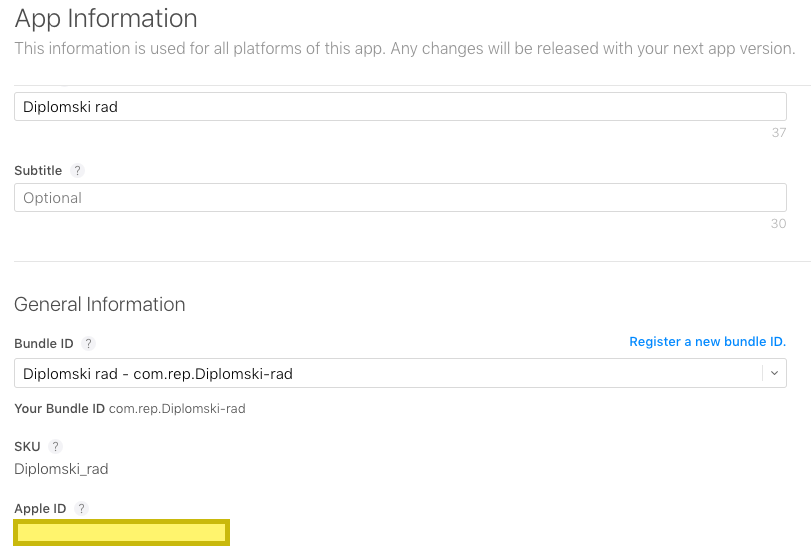
\includegraphics[scale=0.45]{iTunesConnectAppId}
\caption{iTunes Connect profil aplikacije s označenim identifikatorm aplikacije}
\label{fig:iTunesConnectAppId}
\end{figure}

Naredba kreira nekoliko datoteka u \verb|fastlane| direktoriju. Tekstualna datoteka \verb|Deliverfile| pohranjuje podatke vezane uz objavu aplikacije na App Store platformi kao što su korisničko ime Apple Developer računa te identifikator aplikacije. Direktorij \verb|metadata| sadrži nekoliko dokumenata koji omogućavaju jednostavan unos podataka koji će se koristiti prilikom isporuke aplikacije na App Store platformu. Na primjer, pomoću dokumenta \verb|description.txt| je moguće unijeti opis aplikacije. Dodatno, moguće je kreirati zaseban opis za svaki jezik koji Apple podržava.

Nakon inicijalizacije dodatka je isporuku moguće obaviti jednostavno pozivom \verb|deliver| alata. Naravno, kreirana arhiva mora biti potpisana certifikatima i profilima za isporuku na App Store platformi.

Staza \ref{listing:AppStoreLane} implementira cijeli proces isporuke aplikacije na App Store platformu.

\begin{lstlisting}[caption=Isporuka na App Store platformu korištenjem dodatka deliver, label=listing:AppStoreLane]
lane :release do
    match(type: "appstore")
    gym(scheme: "Production", export_method: "app-store")
    deliver
end
\end{lstlisting}

Staza korištenjem dodatka match dohvaća potrebne certifikate i profile, pomoću dodatka gym izgrađuje arhivu aplikacije te na kraju arhivu objavljuje koristeći deliver dodatak.



\chapter{Kontinuirana isporuka} \label{header:KontinuiranaIsporuka}

Kontinuirana isporuka \eng{continuous deployment} je praksa u sklopu programskog inženjerstva koja automatskom isporukom programske potpore nastoji olakšati proces i povečati učestalost isporuke razvijenih funkcionalnosti. Slično kao što kontinuirana integracija automatski obavlja proces integracije za svaku novu verziju repozitorija, tako i kontinuirana isporuka automatski obavlja proces isporuke za svaku novu verziju repozitorija. Međutim, dok kontinuirana integracija nad svakom verzijom obavlja isti proces integracije, kontinuirana isporuka provodi nekoliko različitih procesa isporuke.

Automatizacija procesa isporuke zahtjeva prethodnu implementaciju procesa isporuke. U sklopu rada koristim proces isporuke definiran u sklopu kontinuirane dostave, odnosno u poglavlju \ref{header:KontinuiranaDostava}. Jednako tako proces isporuke zahtijeva prethodnu implementaciju procesa integracije. Zbog navedenog se kontinuirana isporuka može smatrati nastavkom kontinuirane dostave i samim time nastavkom na kontinuiranu integraciju. Razlika između kontinuirane dostave i kontinuirane isporuke je prikazana na slici \ref{fig:CDDifferences}\citep{cd:whats_the_diff}.

\begin{figure}
\centering
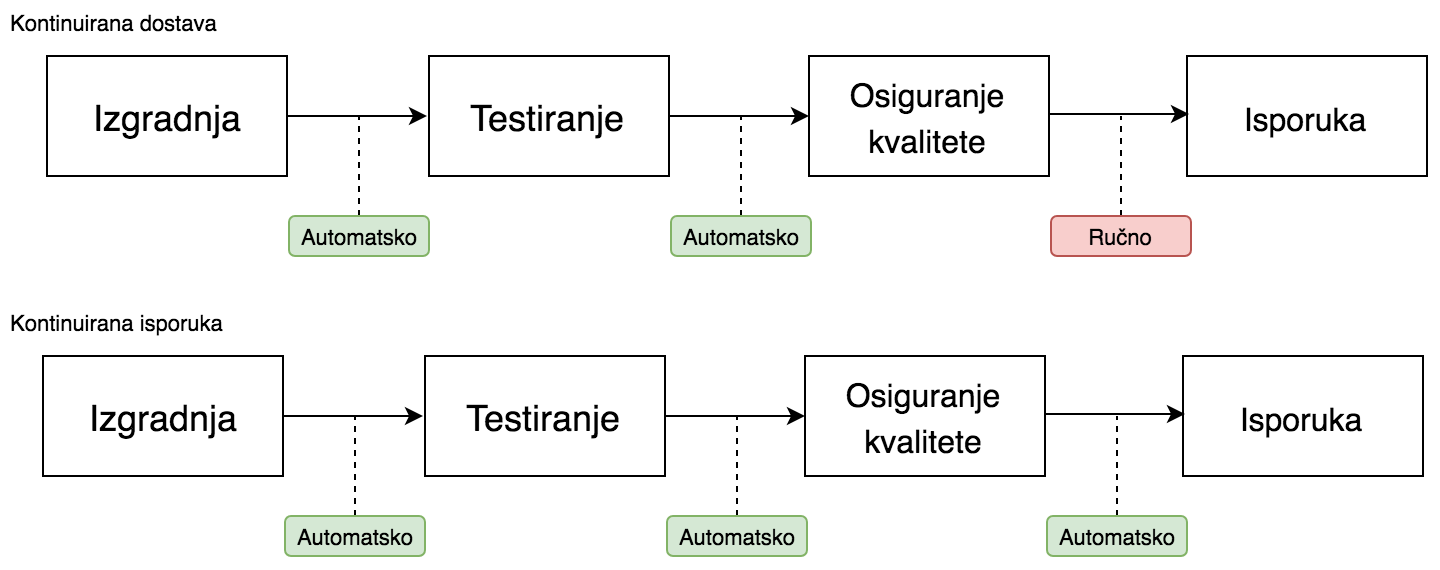
\includegraphics[scale=0.55]{CDDifferences}
\caption{Usporedba kontinuirane dostave i kontinuirane isporuke}
\label{fig:CDDifferences}
\end{figure}

Kontinuirana isporuka je vrlo mlada praksa. Termin je prvi puta iskoristio poznati autor Kent Beck u raspravi o agilnom razvoju programske potpore. Kent Beck je neisporučenu funkcionalnost usporedio s inventarom koji nije prikazan korisniku. Termin kontinuirana isporuka je prvi puta definiran u članku \textit{The Deployment Production Line} autora Jez Humblea, Chris Reada i Dan Northa\citep{mics:DPT}. Danas praksu razvija i unaprjeđuje uglavnom zajednica web programera koji ju, zbog jednostavnosti isporuke programske podrške za web poslužitelje, mogu jednostavno implementirati.

Isporuka programske podrške za web poslužitelje ima značajnu prednost u usporedbi s ostalom programskom potporom. Najvažnije, web aplikacije nije potrebno instalirati na uređaj. Korisnik promjene vidi čim su one dodane na poslužitelju. Dodatno, razvojni tim može direktno upravljati koju će verziju programske potpore korisnik vidjeti. U usporedbi, isporuka iOS aplikacija prvo mora proći provjeru Apple tima te zatim korisnik mora novu verziju preuzeti na uređaj.

\textit{Intercom}, novonastala kompanije bazirana u Irskoj je proces kontinuirane isporuke implementirala krajem 2012. godine. Uz automatizirano obavljanje isporuke, kompanija u sklopu procesa implementira i brojne složeniji funkcionalnosti. Na primjer, kompanija isporuku obavlja u fazama. Umjesto isporuke nove promjene svim korisnicima, promjene vidi samo manji postotak iskusnih korisnika. U blogu objavljenom 2016. godine bilježi stabilan porast broja dnevnih isporuka promjenu od produkcija. Od ispod 10 isporuka u 2012. godini, do preko 80 isporuka u 2015. godini. Slika \ref{fig:IntercomShipsPerDay} prikazuje broj dnevnih isporuka promjena u produkciju kompanije \textit{Intercom}\citep{intercom:cd}.

\begin{figure}
\centering
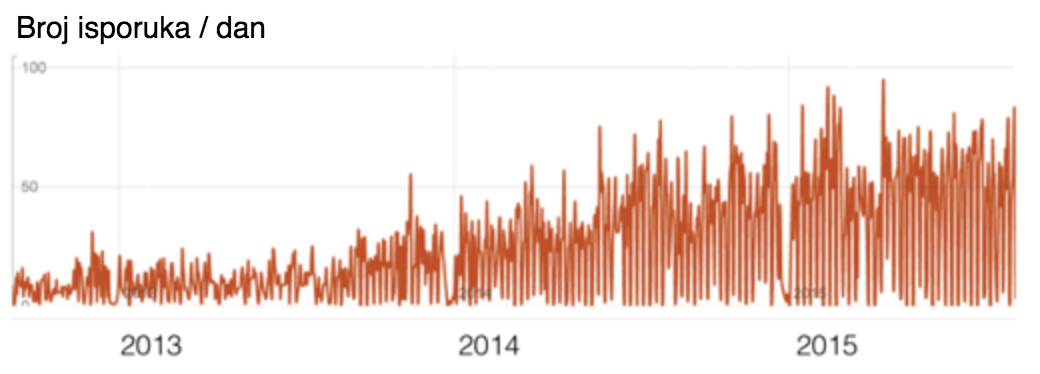
\includegraphics[scale=0.7]{IntercomShipsPerDay}
\caption{Broj dnevnih isporuka promjena u produkciju kompanije \textit{Intercom}}
\label{fig:IntercomShipsPerDay}
\end{figure}

Na žalost, praksa je puno slabije zastupljena u razvoju programske potpore za iOS operacijski sustav. Postoji nekoliko neslužbenih objava u kojima članovi zajednici raspravljaju o procesu automatizacije, međutim navedeni su procesi značajno reducirani u usporedbi s procesima koji se kriste u razvoju programske potpore za web platformu.

\section{Tipovi isporuke}

Ovisno o potrebama tima, kontinuirana isporuka može automatsku isporuku obavljati i za do desetak različitih verzija programske potpore. Navedeni broj verzija se koristi zbog osiguranja kvalitete programske potpore. Nema smisla tek razvijenu funkcionalnost objaviti direktno krajnjim korisnicima. Funkcionalnost je prvo potrebno testirati te osigurati njenju spremnost za objavu u produkciji. Umjesto direktne isporuke nove verzije u produkciju, ista prolazi nekoliko stupnjeva provjere ispravnosti. Drugim riječima, verzija se isporučuje korištenjem nekoliko različitih procesa isporuke. U sklopu rada isporučujem četiri verzije programske potpore: produkcijsku, pripremnu, testnu i razvojnu verziju. Tipovi i redoslijed isporuke verzija je prikazana na slici \ref{fig:DeploymentStages}.

\begin{figure}[h]
\centering
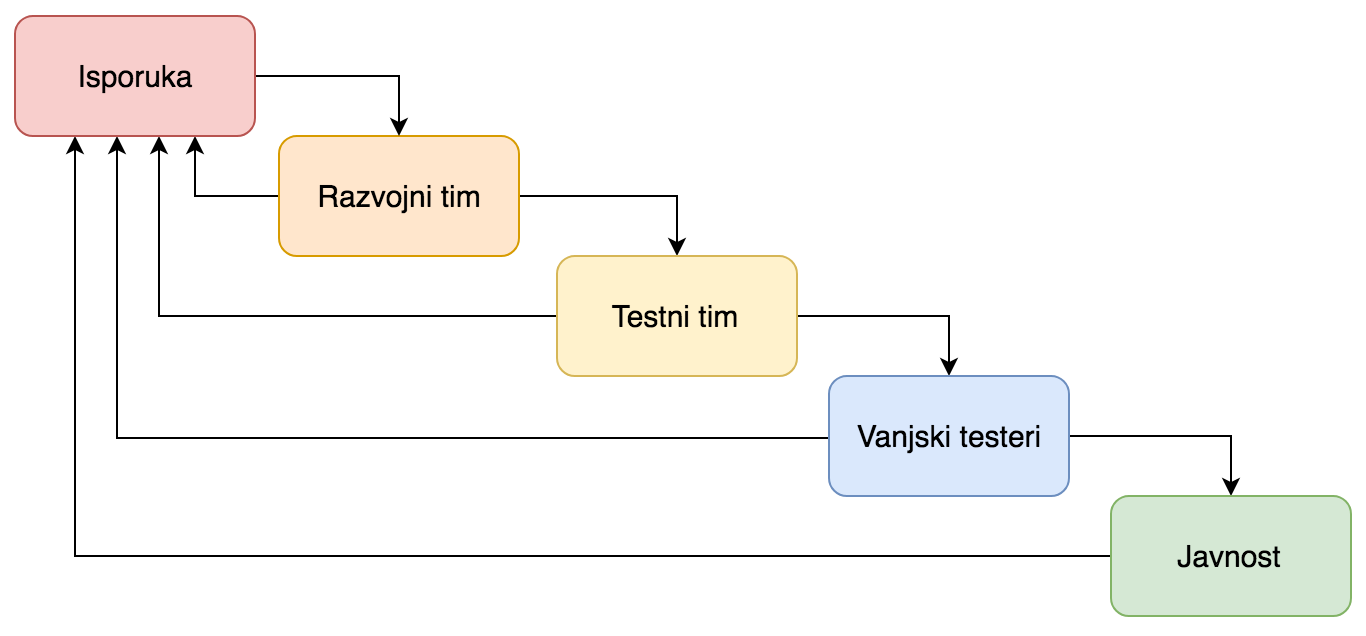
\includegraphics[scale=0.6]{DeploymentStages}
\caption{Postupna isporuka programske potpore skupovima korisnika}
\label{fig:DeploymentStages}
\end{figure}

Razvojna verzija programske potpore prikazuje najnovije stanje aplikacije. Razvojna verzija sadrži najnovije implementirane izmjene koje još nisu nužno prošle proces osiguranja kvalitete. Ovu verziju aplikacije koriste članovi tima za provjeru razvijenih funkcionalnost.

Testnu aplikaciju koristi tim za osiguranje kvalitete kako bi osigurao ispravnost novo razvijenih funkcionalnosti. Kako bi osigurao ispravnost tim provjerava sve izmjene ostvare od zadnje verzije aplikacije. Zbog navedenog je poželjno da je broj izmjena između verzija mali ali dobro dokumentiran. Verzija ovog tipa aplikacije se osvježava otprilike jednom tjedno.

Pripremna verzija aplikacije služi za završnu provjeru aplikacije koja se izdaje u produkciju. Za razliku od testne verzije aplikacije koja sadrži funkcionalnosti korištenje samo u testiranju, pripremna aplikacija mora biti identična onoj koja se želi isporučiti. Jedino na ovaj način možemo provjeriti ispravnost aplikacije u produkcijskom okruženju. Verzija aplikacije se kreira jednom kad tim odluči objaviti novu produkcijsku verziju.

Produkcijska aplikacija je aplikacija trenutno dostupna korisniku. Učestalost isporuke ovisi o timu ali je se zbog Appleovog procesa provjere gotovo nikad ne obavlja češće od jednom tjedno.

Iz navedenog je jasno da trenutan proces ne slijedi principe kontinuirane isporuke. Spor proces izdavanja promjena u produkciju rezultira većim brojem ljudskih pogrešaka i lošijim iskustvom korisnika. Zbog navedenog automatizacijom procesa ne samo da pokušavam smanjiti vrijeme koje tim ulaže u isporuku, već i smanjiti period između dvije isporuke.


\section{Odabir tipa isporuke}

Međutim, kako odrediti koju verziju repozitorija objaviti kojim tipom isporuke? Kako bi istovremeno implementirao isporuku različitih verzija aplikacije te zadržao fleksibilnost razvoja koristm modificirani Gitflow tok rada.

Standardni Gitflow proces sadrži tri grane: glavnu, razvojnu i pripremnu granu. Glavna grana \eng{master branch} predstavlja trenutno stanje programske potpore u produkciji. Svaka verzija ove grane je obilježena oznakom koja sadrži ljudski čitljivu verziju aplikacije i popis promjena obavljenih od prošle verzije. Razvojna grana \eng{develop branch} predstavlja trenutno stanje aplikacije u razvoju. Objava promjena u produkciju se obavlja korištenjem pomoćne pripremne grane koja se kreira iz razvojne grane. Nakon provjere ispravnosti promjena iste se dodaju glavnoj grani i time objavljuju u produkciju. Nove funkcionalnosti se razvijaju u zasebnoj grani koja se za potrebe razvoja funkcionalnosti kreira iz razvojne grane te se po završetku razvoja u nju spaja. Pregled cijelog procesa je dostupan u odlomku \ref{header:Implementacija_verzioniranja}.

Uz navedene grane koristim i testnu granu koja služi za održavanje i isporuku testne aplikacije. Kako bi olakšali i poboljšali proces testiranja, korisno je testne verzije objavljivati sistematizirano. Nova testna verzija se kreira spajanjem svih verzija dodanih razvojnoj grani od zadnjeg kreiranja testne verzije. Sve promjene dodane u sklopu ove testne verzije je potrebno jasno specficirati. Greške koje se otkriju u sklopu testiranja se otklanjaju na testnoj grani te se po završetku testiranja spajaju s razvojnom granom. Slika \ref{fig:GitFlowCD} prikazuje proces automatizirane isporuke korištenjem \textit{gitflow} procesa.

\begin{figure}[t!]
\centering
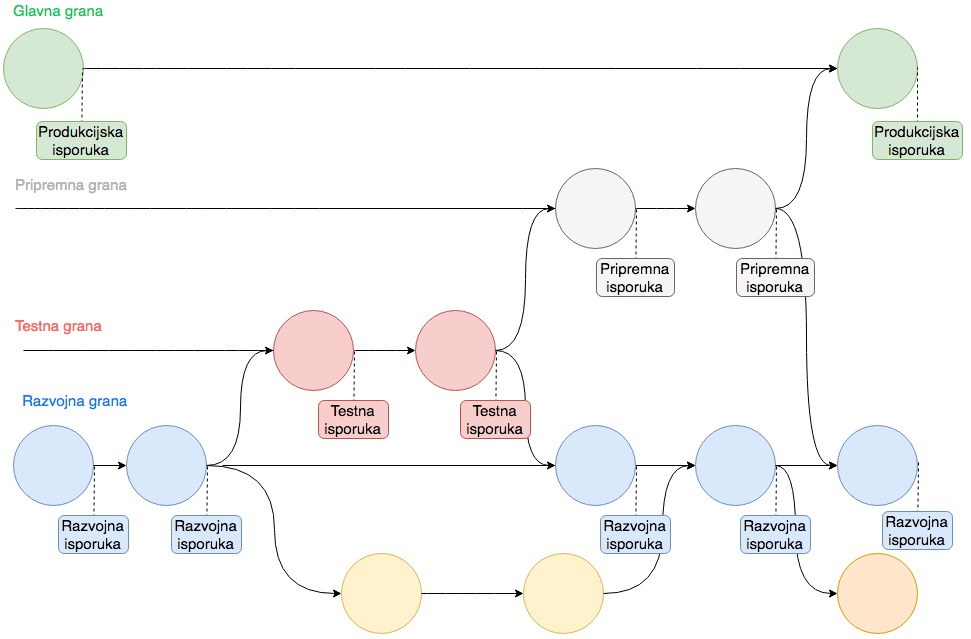
\includegraphics[scale=0.5]{GitFlowCD}
\caption{Automatska isporuka primjenom \textit{gitflow} procesa}
\label{fig:GitFlowCD}
\end{figure}

Sada je vrlo jednostavno odrediti koji tip isporuke iskoristiti za koju verziju repozitorija. Ukoliko se izmjena nalazi na razvojnoj grani potrebno je osvježiti razvojnu verziju aplikacije a ako se izmjena nalazi na testnoj grani potrebno je osvježiti testnu verziju.

\begin{figure}[b!]
\centering
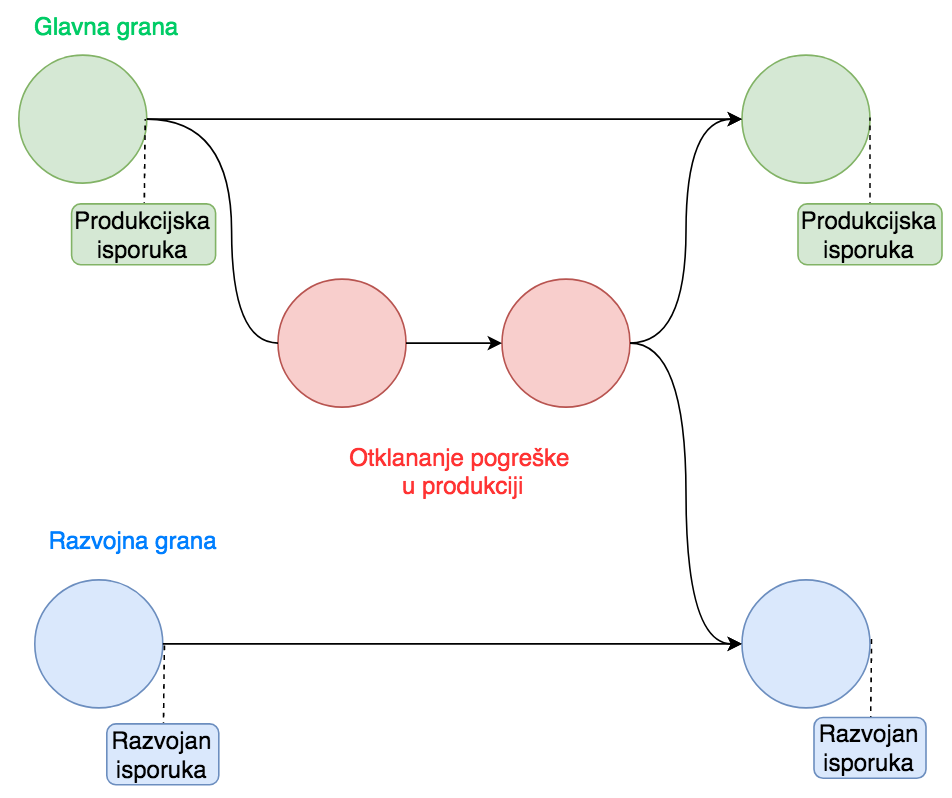
\includegraphics[scale=0.5]{HotfixGitflow}
\caption{Automatska isporuka otklananja pogreške u produkciji}
\label{fig:HotfixGitflow}
\end{figure}

U praksi se često javljaju novi, neočekivani zahtjevi. Jedan od primjera ovog tipa zahtjeva je otkrivanje pogreške u produkcijskoj verziji koju je odmah potrebno ukloniti. Budući da razvojna grana sadrži promjene koje još nisu objavljene na produkciji, grešku nije moguće otkloniti sljedeći standardnu praksu. Međutim, moguće je granu za otklanjanje pogreške kreirati direktno iz glavne grane. Nakon otklanjanja pogreške i testiranja, promjena se spaja s glavnom granom čime se ista objavljuje u produkciju i s radnom granom. Primjer otklanjanja greške u produkciji se nalazi na slici \ref{fig:HotfixGitflow}. Važno je prilikom pojave zahtjeva ovog tipa iskoristiti postojeće procese isporuke.

Skripta \ref{listing:git_branch_creation} prikazuje proces kreiranja potrebnih grana.

\begin{lstlisting}[caption=Kreiranje potrebnih grana Gitflow radnog toka, label=listing:git_branch_creation]
git checkout -b develop
git push --set-upstream origin develop

git checkout -b release-candidate
git push --set-upstream origin release-candidate

git checkout -b test
git push --set-upstream origin test
\end{lstlisting}

\section{Priprema projekta za automatsku isporuku}

Uz različiti proces isporuke, različite verzije aplikacije mogu zahtijevati i različitu konfiguraciju projekta. Na primjer, standardno je testnoj verziji aplikacije dodati funkcionalnosti koje olakšavaju testiranje a nisu dostupne stvarnom korisniku. Dodatno, kako bi na isti uređaj mogli imati više različitih verzija aplikacije, navedene verzije se moraju na neki način razlikovati. iOS operacijski sustav aplikacije razlikuje na temelju identifikatora aplikacije \eng{Bundle Identifier}.

Navedeni tipovi funkcionalnosti se implementiraju konfiguracijom postavka projekta. Svaki cilj iOS projekta sadrži najmanju jednu konfiguraciju projekta \eng{configuration}. Konfiguracija omogućava modifikaciju velikog broja opcija definiranih u procesu kreiranja projekta. Konfiguracija je pohranjena u \verb|.xcodeproj| datoteci zajedno s ostatkom informacija o projektu koja nije pogodna za ručnu izmjenu. Datoteku je najlakše modificirati korištenjem Xcode aplikacije koja konfiguraciju prikazuje u jednostavnom i intuitivnom grafičkom sučelju. Slika \ref{fig:XcodeConfiguration} prikazuje dio opcija konfiguracije prikazanih pomoću Xcode alata.

\begin{figure}
\centering
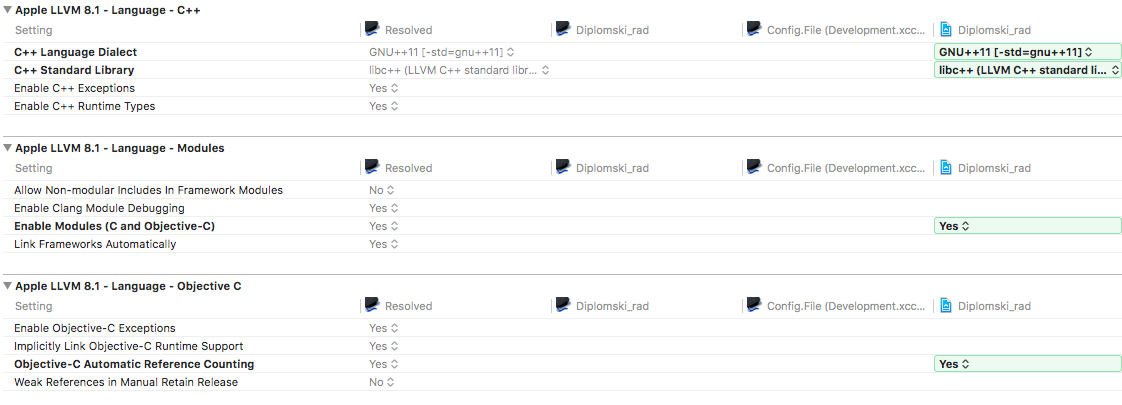
\includegraphics[scale=0.37]{XcodeConfiguration}
\caption{Dio opcija konfiguracije iOS projekta}
\label{fig:XcodeConfiguration}
\end{figure}

Dodatno, projekt može sadržavati više od jedne konfiguracije. Standardno se koristi jedna glavna i više specifičnih konfiguracija. Glavna konfiguracija definira standardna pravila za cijeli projekt. Specifične konfiguracije nasljeđuju glavnu konfiguraciju, izmijenjuju željene postavke te se koriste za konfiguraciju operacija projekta. Slika \ref{fig:XcodeConfigurationCreation} prikazuje proces kreiranja specifične konfiguracije. Kreiranja konfiguracije se ostvaruje dupliciranjem postojećem konfiguracije. Pokrenuti projekt korištenjem Xcode aplikacije te odabrati željenu shemu. U sekciji \verb|Info| te u odjeljku \verb|Configurations| odabirom opcije \verb|Plus| i željene postojeće konfiguracije kreirati konfiguraciju.

\begin{figure}[b!]
\centering
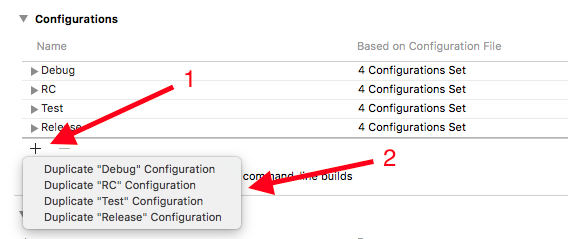
\includegraphics[scale=0.6]{XcodeConfigurationCreation}
\caption{Kreiranje nove konfiguracije Xcode projekta}
\label{fig:XcodeConfigurationCreation}
\end{figure}

Modifikacija postavka pomoću specifične konfiguracije je jednostavna ali je teško pronaći sve specificirane postavke. Dodatno, vrlo je teško pratiti promjenu postavka budući da se iste dodaju \verb|.xcodeproj| datoteci. Zbog navedenog se u praksi često koriste zasebne tekstualne \verb|.xcconfig| datoteke koje specificiraju samo željene opcije. U sklopu rada kreiram četiri \verb|.xcconfig| datoteke. Sadržaj datoteka je prikazan u skripti \ref{listing:xcconfig}. Naredba \#1 dodaje konfiguraciju CocoaPods projekta novo kreiranoj konfiguraciji dok naredba \#2 postavlja vrijednost identifikatora aplikacije. Testna konfiguracija sadrži dodatnu \verb|IS_TEST| opciju koja se koristi za dodavanje testnih funkcionalnosti.

\begin{lstlisting}[caption=Sadržaj .xcconfig datoteke, label=listing:xcconfig]
#include "Pods/Target Support Files/Pods-Diplomski_rad/Pods-Diplomski_rad.debug.xcconfig" #1

PRODUCT_BUNDLE_IDENTIFIER = com.rep.Diplomski-rad.{sufix} #2

IS_TEST = 1 #3
\end{lstlisting}

Kreirane \verb|.xcconfig| datoteke je potrebno dodati konfiguraciji. U sekciji \verb|Info| te u odjeljku \verb|Configurations| odabrati željenu konfiguraciju te za sve ciljeve iskoristiti istu \verb|.xcconfig| datoteku. Slika \ref{fig:XcodeXCConfigSet} prikazuje dodavanje datoteka razvojnoj konfiguraciji.

\begin{figure}
\centering
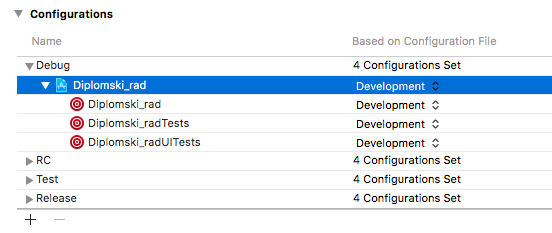
\includegraphics[scale=0.6]{XcodeXCConfigSet}
\caption{Dodavanje .xcconfig datoteke postojećoj konfiguraciji projekta}
\label{fig:XcodeXCConfigSet}
\end{figure}


\section{Implementacija kontinuirane isporuke}

Za dovršenje implementacije je potrebno isporuku pokrenuti korištenjem bota. Prvo je za svaki tip isporuke potrebno kreirati zaseban bot. Najjednostavnije je duplicirati već postojeći bot te promijeniti na kojoj bot pokreće integraciju. Slika \ref{fig:MultipleBots} prikazuje botove korištene u radu.

\begin{figure}[b!]
\centering
\includegraphics[scale=0.7]{MultipleBots}
\caption{Novo kreirani botovi}
\label{fig:MultipleBots}
\end{figure}

Nakon kreiranja botova je potrebno promijeniti konfiguraciju koju botovi koriste te pozvati ispravan proces isporuke.

Konfiguraciju koju projekt koristi je moguće podesiti u postavkama bota. Odabrati opciju \textit{Edit Bot... -> Build Configurations} te za svaki bot odabrati odgovarajuću konfiguraciju.

\begin{figure}
\centering
\includegraphics[scale=0.5]{BotConfiguration}
\caption{Odabir konfiguracije koju bot koristi}
\label{fig:BotConfiguration}
\end{figure}

Isporuku ostvarujem korištenjem fastlane staza definiraniranih u prošlom poglavlju. Stazu je potrebno pokrenuti po završetku obavljanja integracije za što koristim fazu koja se obavlja nakon integracije \eng{Post-integration script}. Odabrati opciju \textit{Edit Bot... -> Triggers} te dodati novu fazu. Odabrati opciju pokretanja jedino u slučaju uspješnog obavljanja integracije. Svaki bot treba pozivati stazu koja implementira željeni tip isporuke. Skripta \ref{listing:bot_fastlane_call} prikazuje sadržaj faze.

\begin{lstlisting}[caption=Sadržaj faze nakon obavljanja isporuke, label=listing:bot_fastlane_call]
#!/bin/bash

cd $XCS_PRIMARY_REPO_DIR #1

export PATH="~/.fastlane/bin:~/com.rep.Diplomski-rad.development:/usr/local/bin:~/.gem/ruby/2.0.0/bin/:$PATH" #2

fastlane {ime_staze} #3
\end{lstlisting}

Naredba \#1 navigira proces u ispravni direktorij, naredba \#2 dodaje potrebne putanje u \verb|PATH| varijablu okruženja, dok nareba \#3 pokreće proces isporuke implementiran pomoću fastlane staze.

\section{Pregled rezultata implementacije kontinuirane isporuke}

\begin{figure}[b!]
\centering
\includegraphics[scale=0.3]{CrashlyticsEmail}
\caption{Crashlytics e-mail poruka izdana nakon objave nove verzije aplikacije}
\label{fig:CrashlyticsEmail}
\end{figure}

Kreiranjem novog stanja repozitorija na razvojnoj, testnoj, pripremnoj i glavnoj grani se pokreće proces integracije i isporuke korištenjem navedenog stanja. Integracija se sastoji od izgradnje, testiranja i osiguranja kvalitete nove verzije aplikacije. Ukoliko se svi procesi ispravno izvrše započinje proces isporuke koji odgovara grani na kojoj je stanje kreirano. Glavna verzija aplikacije se objavljuje na App Store platformi dok se ostale verzije aplikacije objavljuju na Crashlytics platformi.

Navedeni se proces odvija u potpunosti automatizirano.

\begin{figure}[b!]
\centering
\includegraphics[scale=0.3]{Beta}
\caption{Preuzimanje aplikacije s Crashlytics platforme korištenjem aplikacije Beta}
\label{fig:Beta}
\end{figure}

Novu verziju aplikacije je moguće preuzeti s Crashlytics platforme desetak minuta nakon kreiranja novog stanja repozitorija. Svaka osoba dodana kao tester aplikacije dobiva e-mail poruku pomoću koje može preuzeti aplikaciju. Na željenom mobilnom uređaju otvoriti dobivenu e-mail poruku te odabirom opcije \verb|Let Me In| započeti proces preuzimanja nove verzije aplikacije. Slika \ref{fig:CrashlyticsEmail} prikazuje dobivenu e-mail poruku.

Instalacija aplikacija objavljenih na Crashlytics platformi se obavlja pomoću aplikacije \textit{Beta}. Ako aplikacija već nije  instalirana na mobilnom uređaju, opcija pokreće proces instalacije i konfiguracije navedene aplikacije. Slika \ref{fig:Beta} prikazuje izgled ekrana aplikacije Beta s kojeg je moguće preuzeti objavljne aplikacije. Odabirom opcije \verb|Install| se pokreće instalacija nanovije verzije aplikacije. Moguće je preuzeti i neku od starijih verzija.

S druge strane, verzija objavljena na App Store platformi prvo mora proći Appleovu provjeru. Ako provjera uspješno završi aplikaciju je potrebno objaviti korištenjem iTunes Connect platforme. Navedeni proces trenutno nije moguće automatizirati. Nakon objave je nova verzija vidljiva na App Store platformi te se već instalirane aplikacije samostalno osvježavaju.

\chapter{Zaključak}

Kontinuirana isporuka je tek u svojim začecima u iOS zajednici. Iako praksa dobiva sve više pozornosti, trenutno ne postoji dovoljna potpora zajednice i vodečih kompanija. Implementcija čak i najosnovnih funkcionalnosti je teška, zahtijeva kombinaciju nekoliko različitih alata te sadrži veliki broj pokušaja i pogreška. Dodatnu, u praksi situacija nikad nije ovako jednostavna. Gotovo svaki tim definira vlastiti način rada a izuzeci se koriste čak i u najbolje organiziranim timovima.

Iako je implementacija zahtijevna, benefiti kontinuirane isporuke značajno olakšava razvoj. Automatska isporuke novih promjena u potpunosti eliminira potrebnu obavljanja ručne isporuke. Ručna isporuke iziskuje utrošak ljudskih resursa. Ovisno o timu i zahtjevima razvoja, proces može zauzeti i do desetak posto ukupnog vremena. Utrošak je posebno visok u timovima koji koriste agilni pristup razvoju. Ovaj pristup učestalom isporukom i kominikacijom s klijentom nastoji osigurati izgradnju ispravnog produkta, ali upravo navedena učestala isporuka zahtijeva utošak značajnog dijela vremena. Kontinuirana isporuka u potpunosti eliminira ovaj zadatak.

Najvažnije, korištenje kontinuirane isporuke gotovo upoče ne mijenja postoječi proces razvoja programske potpore. Proces jednostavno verziju već integriranu procesom kontinuirane integracije objavljuje željenim tipom isporuke. Jedino što je potrebno definirati je koju verziju repozitorija objaviti kojim tipom isporuke. U sklopu rada koristim Gitflow tok rada ali je isto moguće ostvariti na više načina, na primjer označavanjem postoječih verzija repozitorija.

Glavni cilj kontinuirane isporuke je automatizacijom isporuke povečati njenu učestalost i time poboljšati kvalitu produkta. Iako automatizacija procesa omogučava češću objavu, potrebno je izmijeniti i cijeli pristup razvoju. Trenutno je vrlo rijetko verziju iOS aplikacije osvježiti češće od jednom tjedno čak i u timovima s velikim brojem članova. Navedenom problemu dijelom pridonosi Appleov proces provjere novih verzija, ali dijelom i nerazumijevanje razvojnog tima. Razvijene funkcionalnosti se nastoje grupirati i objaviti zajedno, umjesto njihove pojedinačne isporuke. Vođen primjerom web razvoja je za očekivati da će se navedeni problem riješiti sam od sebe. Olakšavanjem isporuke očekujem postupno povečanje učestalosti isporuke slično brojkama zabilježenim u zadnjem desetlječu razvoja web aplikacija.

U sklopu rada sam implementirao kontinuiranu isporuku za programsku potporu za iOS operacijski sustav. Kontinuiranu integraciju i automatsko pokretanje isporuke sam implementirao korištenjem aplikacije Xcode Servera, dok sam isporuku implementirao korištenjem alata fastlane. Alat implementira isporuku četiri verzije aplikacije uz objavu na App Store i Crashlytics platformu.

S druge strane, za alat Xcode Server imam puno manje pohvala. Glavna mana alata proizlazi iz činjenice da je on namjenjen za jednostavnu implementaciju kontinuirane za iOS operacijski sustav. Navedena jednostavnost značajno otežava proširenje osnovnog seta funkcionalnosti. Osnovan problem leži u sučelju alata koje je za razliku večine sličnih alat grafičko. Navedeno značajno otžava proces kreiranja procesa buduči da je sve korake potrebno obaviti ručno.

Prije prihvačanja kontinuirane isporuke kao sastavnog dijela razvoja je potrebno olakšati proces implementacije.




\bibliography{literatura}
\bibliographystyle{fer}

\begin{sazetak}

Kontinuirana isporuka je praksa u programskom inženjerstvu koja automatskim obavljanjem isporuke programske potpore nastoji povečati njenu učestalost i time povečati kvalitetu razvijenog produkta. Kontinuirana isporuka se direktno nastavlja na kontinuiranu dostavu, praksu koja automatiziranjem procesa isporuke nastoji olakšati njegovo obavljanje. Praksa nastoji osigurati mogučnost isporuke programske potpore u bilo kojem trenutku uz minimalnu količinu rada. Obje prakse su razvijene na temelju te se direktno nastavljaju na kontinuiranu integraciju, praksu automatskog obavljanja integracije nad svakom promjenom izvornog koda. Ove tri prakse nastoje olakšati timski razvoj, poboljšati kvalitetu koda i produkta te ubrzanjem i automatizacijom isporuke ubrzati objavu novih funkcionalnosti.

Rad definira kontinuiranu integraciju, dostavu i isporuku iz perspektive razvoja za iOS operacijski sustav, ustanovljava zahtjeve koji se javljaju u praksi te implementira sustav koji zadovoljava ustanovljene zahtijeve. Kako bi sustav opravdao korištenje on mora biti prenosiv, jednostavna za implementaciju i svakodnevno korištenje. Sustav je implementiran korištenjem aplikacije Xcode Server i alata fastlane.

Rezultat rada je u automatska integracija i isporuka svake nove verzije repozitorija čime eliminiram potrebu za obavljanje ručne isporuke.

\kljucnerijeci{Ključne riječi, odvojene zarezima.}

Kontinuirana isporuka, kontinuirana dostava, kontinuirana izgradnja, Xcode Server, fastlane

\end{sazetak}

\engtitle{Implementation of Continuous Deployment for iOS Operating System}

\clearpage


\begin{abstract}

Continuous Deployment is a software engineering approach which by deploying software automatically tries to increase frequency and quality of deployed product. Continuous Delivery is a direct extension of Continuous Delivery, an approach that tries to automate the whole process of product delivery in order to reduce its complexity. Additionally, Continuous Delivery ensuring that the software can be reliably released at any time. Both approaches were developed on top of Continuous Integration which automatically performs integration process for every new repository state. These three practices aim to simplify teamwork, improve quality of code and product, and shorten the process of delivery.

This thesis defines approaches of Continuous Integration, Continuous Delivery and Continuous Deployment from the perspective of development for iOS operating system, to recognize requirements which occur in the real worl and to implement a system that satisfies them. In order for a system to usable, it needs to be easily transferable and simple to implement and use. The system is implemented using Xcode Server application and fastlane tool.

The result of the thesis is automated integration and delivery of every new repository version thus eliminating need to perform delivery by hand.

\keywords{Keywords.}

Continuous Deployment, Continuous Delivery, Continuous Integration, Xcode Server, fastlane

\end{abstract}


\begin{appendices}

\chapter{Usporedba alata za implementaciju kontinuirane integracije} \label{header:dodatak_usporedba_alata_za_kontinuiranu_integraciju}

Kontinuirana integracija je ustaljena i dobro prihvaćena praksa u sklopu razvoja programske potpore. Jedan od glavnih razloga njene prihvačenosti je postojanje velikog broja alata koji značajno olakšavaju njenu implementaciju.

Međutim, navedeni alati se međusobno značajno razlikuju. Dok neki alati nastoje podržati što veči broj funkcionalnosti za što više tehnologija, drugi se fokusiraju na pojedinu instancu razvojnog procesa. Neki sustavi se ističu u svojoj jednostavnosti, dok drugi pružaju veću fleksibilnost.

Cilj ovog dodatka je korištenjem i ocjenom četiri trenutno najpopularnija alata ustanoviti koji najbolje odgovara zahtjevima kontinuirane integracije za iOS operacijski sustav. U sklopu dodatka rankiram četiri alata: Jenkins, Travis CI, CircleCI i Xcode Server.

Uz ovoliku količinu gotovih rješenja je teško naći argument za razvoj vlastitog rješenja. Gotovo sve implementacije kontinuirane integracije koriste neki od postojećih alata. Čak i kada tim krene u razvoj vlastitog rješenja, najčešće modificira ili proširuje već postojeće alate otvorenog koda.

Međutim, teško je iz navedene količine dostupnih sustava izabrati onaj koji najviše odgovara zahtjevima tima te u isto vrijeme zahtjeva najmanje truda za implementaciju i korištenje. Javno dostupni dokumenti ne pomažnu zmačajno u ovom pitanju. S ciljem boljeg razumijevanja danog problema i jednostavnije procjene karakteristika sustava kontinuirane integracije provodim ispitivanje sustava korištenjem dva jednostavna upitnika. Rezultati upitnika su isključivo moja procjena te je njihova glavna svrha bolja organizacija i lakša procjena karakteristika sustava.

Oba upitnika se zajedno s ocjenama sustava nalaze na kraju dodatka.

\section{Prvi upitnik}
Prvo upitnik procjenjuje koliko dobro sustav zadovoljava funkcionalnosti opisane u prethodnom poglavlju. Kako bi se lakše provelo ocjenjivanje te rezultati bili bolje razumljiviji, pitanja su podijeljena u pet kategorije.

Prva kategorija, \textit{opći zahtjevi}, specificira koliko je lako sustav uklopiti u postojeći proces razvoja programske potpore. U ovo poglavlje ubrajamo mogućnost integracije sustava sa sustavima za kontrolu verzija i mogućnost integracije u postojeći proces razvoja. Poželjno je sustav kontinuirane integracije ostvariti ne mijenjajući postojeći proces razvoja.

Druga kategorija, \textit{provjera ispravnosti}, ispituje podržava li sustav sve zahtjeve automatizacije provjere ispravnosti integracije. Ovi se zahtjevi sastoje od automatiziranja izgradnje, testiranja i osiguranja kvalitete. Dodatno, kategorija ocjenjuje konfigurabilnost testne okoline i mogućnost testiranja na stvarnim uređajima.

Treća kategorije, \textit{izvršavanje procesa}, provjerava koliku slobodu sustav pruža pri definiranju i obavljanju procesa. Kategorija promatra kada je moguće pokrenuti procese te pruža li sustav napredne mogućnosti ulančavanja procesa i stvaranje ne standardnih procesa.

Četvrto poglavlje, \textit{rezultati procesa}, prikazuje u kojem stupnju sustav podržava automatsko izvještavanje te koliko je dostupan i detaljan pregled rezultata procesa.

Peto poglavlje, \textit{kontinuirana dostava i isporuka}, daje uvid stupnja u kojem sustav podržava željene funkcionalnosti kontinuirane dostave i isporuke.

Svaka se točka upitnika ocjenjuje brojčanom ocjenom od 0 do 5. Ocjena 0 znači da sustav ne podržava danu funkcionalnost, dok ocjena 5 znači da sustav podržava danu funkcionalnost bez potrebne dodatne modifikacije \eng{off the shelf}. Ocjene od 1 do 4 označavaju da je funkcionalnost podržavana, ali je potrebna različita količina truda za njezinu implementaciju. Ocjena 1 označava da je funkcionalnost jako teško implementirati, dok ocjena 4 označava da je funkcionalnost jednostavno implementirati.

Upitnik ne daje definitivnu ocjenu sustava, već služi za generalnu navigaciju po širokom tržištu alata kontinuirane integracije. Uz ukupan rezultat pojedinog sustava, korisno je promatrati i rezultate pojedine kategorije.

\section{Drugi upitnik}
Drugi se upitnik fokusira na jednostavnost korištenja, implementacije i održavanja sustava iz perspektive razvoja programske podrške za mobilne operacijske sustave. Cilj ovog ispitivanje je procijeniti koliko je složeno implementirati odabrani sustav kontinuirane integracije za postojeće proces razvoja programske potpore za mobilne operacijske sustave.

Na tržištu trenutno dominiraju tri mobilna operacijska sustava: Android, iOS i Windows Phone. U sklopu ovog rada preskačem Windows Phone zbog neizvjesnosti nastavka njegove primjene.

Kod razvoja programske potpore za iOS i Android prepoznajemo nekoliko različitih procesa razvoja i korištenih tehnologija. Najkorišteniji su procesi vezani uz odvojeni razvoj korištenjem službenih alata i tehnologija. Za iOS to je Xcode IDE s Objective-C ili Swift programskim jezicima, dok je za Android to Android Studio IDE i programski jezik Java. Alternativna opcija razvoja aplikacija za mobilne platforme je više platformski razvoj \eng{cross-platform} koji omogućuje potpunu ili djelomičnu ponovnu iskoristivost koda na više platformi. Prvi pristup je puno popularnije te pruža značajno šire mogućnosti razvoja. Zbog toga se u sklopu ovog rada fokusiram prvenstveno na odvojeni pristup razvoju. Međutim, zaključci do kojih dolazi ovo poglavlje se s manjim ograničenjem mogu preslikati na više platformski razvoj.

Poželjno je isti sustav kontinuirane integracije iskoristiti za oba razvojna procesa. Međutim, kako su određeni sustavi specijalizirani za određeni proces, oni istovremeno mogu biti vrlo dobri za jedan, a vrlo loši za drugi razvojni proces.

Upitnik se sastoji od sljedećih pitanja:

\begin{easylist}

& jednostavnost korištenja
& jednostavnost ugradnje
& jednostavnost konfiguracije
& jednostavnost održavanja

\end{easylist}

pri čemu se svaka stavka ocjenjuje ocjenom od 1 do 5, gdje 1 znači vrlo složeno a 5 vrlo jednostavno. Poredak sugerira važnost pojedine stavke na temelju prethodnog iskustva.

\section{Ispitani sustavi}
Sustave za kontinuiranu integraciju generalno možemo podijeliti u dvije grupe. \textit{SaaS, Software as a Service} alati su hostani od strane davatelja usluge. Navedeni alati zahtijevaju minimalnu konfiguraciju, dostupni su prema potrebi korisnika te su jednostavni za korištenje. Međutim, oni uglavnom pružaju predefinirani i ne fleksibilan set funkcionalnosti. Dostupni su uglavnom kao aplikacije za web poslužitelje koje dodatne mogućnosti omogućuju pružanjem fleksibilnog programskog sučelja \eng{Application Interface, API}. Drugi tip alata su samostalno hostani alati koje korisnik podiže na vlastitom računalu. Ovi tipovi sustavi su fleksibilniji te korisniku pružaju napredne funkcionalnosti, ali zahtijevaju veći napor za postavljanje, održavanje i korištenje.

Kroz ovu cjelinu detaljno promatram po dva sustava iz pojedine kategorije. Odabrani sustavi se ubrajaju među najpoznatije i najkorištenije sustave kontinuirane integracije. Smatram da ovaj mali skup pokriva većinu zahtjeva koje sam definirao u drugom poglavlju ovog rada, odnosno, većinu stvarnih potreba razvoja programske potpore za mobilne sustave.

\subsection{Jenkins}

Jenkins je najpopularniji samostalno hostani CI sustav. Golemu popularnost je zaslužio zbog velike fleksibilnosti i kompatibilnosti s gotovo svim alatima korištenim u razvoju programske potpore. Jenkins je moguće koristiti kao generički sustav kontinuirane integracije ili ga pretvoriti u složeni sustav koji podržava specifične zahtjeve pojedinog tima. Navedena fleksibilnost je ostvarena \textit{plugin arhitekturom}. Pluginovi, koji se jednostavno razvijaju i spajaju s osnovnim sustavom, omogućuju integraciju Jenkinsa s bilo kojom tehnologijom i razvojnim procesom. Danas postoje stotine pluginovi koji omogućavaju jednostavnu integraciju Jenkinsa s gotovo svim IDEovima, sustavima za kontrolu verzija i bazama podataka\citep{wiki:Jenkins}.

Jenkins je sustav otvorenog koda, originalno razvijen u kompaniji \textit{Sun Microsystems} pod imenom \textit{Hudson}\citep{wiki:Hudson} 2004. godine. Ubrzo je stekao popularnost kao bolji od tada dostupnih poslužitelja za izgradnju programske podrške \eng{build server}. Između Hudsonove zajednice i vlasnika, kompanije \textit{Oracle}, se 2010. godine pojavio mali problem oko korištene infrastrukture. Problem je prerastao u široku raspravu oko vlasništva i kontrole nad sustavom. Iako su se zajednica i Oracle slagali u velikom broju pitanja, vlasništvo nad imenom “Hudson” je postao nepremostivi problem.  Zajednica je u siječnju 2011. objavila poziv na glasanje za izmjenu imena projekta iz “Hudson”u “Jenkins”. Izmjena je usvojena velikom većinom glasova te je osnovan projekt Jenkins. Oracle nastavlja razvoj Hudsona odvojeno od Jenkinsa, međutim, bez podrške zajednice Hudson značajno zaostaje u razvoju i popularnosti.

Jenkins je odličan ako je timu potrebna velika razina kontrole nad procesom automatizacije. Ova razina kontrole može donijeti značajnu korist timu i, u cijelosti, olakšati i poboljšati proces razvoja programske potpore. Naravno, visoka razina kontrole otežava postavljanje, održavanje i korištenje sustava.

Jenkins je na prvom ocjenjivanju ostvario 44 od ukupno 60 bodova. Najlošije ostvaruje 5. kategoriju zbog nepostojanja jednostavnog načina podjele korisnika i automatske isporuke. Ovo je očekivano kako je Jenkins jedan od najfleksibilnijih alata trenutno dostupnih na tržištu, međutim zahtjeva puno programiranja te je složen za svladavanje.

Na drugom ocjenjivanju je sustav ocijenjen puno lošije. Jenkins je skupio 11/20 bodova iz perspektive mobilnih sustava. Sustav je jednostavan za korištenje, međutim vrlo složen za ugradnju i konfiguriranje. Potrebno je uložiti barem 20 sati kako bi programer postao upoznat s osnovama sustava i njegovog korištenja. Međutim, postoje vrlo dobri pluginovi koji podržavaju razvoj aplikacija za iOS u Xcodeu i aplikacija za Android u Android Studiju koji ovaj problem djelomično otklanjanju.

Jenkins je jedno od najboljih rješenja za kontinuiranu integraciju ako je tim spreman uložiti nekoliko mjeseci rada za ostvarivanje sustava kontinuirane integracije. Mogućnosti su gotovo beskonačne a velika zajednica koja ga okružuje čini implementaciju puno lakšom.

\subsection{Xcode Server}

Xcode Server omogućava vrlo jednostavnu kontinuiranu integraciju za korisnike programskog alata Xcode, odnosno za razvoj aplikacija za iOS i OS X operacijske sustave. Xcode Server je kombinacija dva alata, Xcodea, alata za razvoj iOS i OS X aplikacija, te OS X Servera, alata za automatizaciju razvojnog procesa. Xcode Server omogućava automatiziranu integraciju, izgradnju, testiranje, analizu i arhiviranje aplikacija. Također omogućava automatsku dojavu rezultata i generiranje statistika za velik broj parametara.

Xcode Server, Appleov alat za kontinuiranu integraciju, je po mnogima najbolji sistem za kontinuiranu integraciju iOS i OS X aplikacija. Xcode Server se razvija kontinuirano uz Xcode. Za razliku od ostalih alata, sve su nove funkcionalnosti potrebne za integraciju Xcode projekata dostupne na dan njihovog izdavanja. Ova je funkcionalnost vrlo korisna pri ranom testiranju novih verzija sustava te se pokazala vrlo korisnom u mnogim projektima.

On je, kao i Jenkins, samostalno hostan i fleksibilan sustav. Funkcionalnosti se implementiraju izgradnjom \textit{botova} koji zatim pokreću zadani proces. Procesi su implementirani korištenjem jezika korištenog u razvoju iOS i OS X aplikacija. Zbog korištenja istog alata i istog jezika kao i za razvoj iOS aplikacija, implementiranje kontinuirane integracije korištenjem Xcode Servera je vrlo jednostavno programerima upoznatima s razvojem iOS aplikacija. Navedeno značajno olakšava implementaciju koja tada zahtjeva značajno manje od implementacije Jenkins sustava.

Dodatna prednost Xcode Servera je mogućnost automatske instalacije aplikacije na testne uređaj te lako praćenje i nadzor instaliranih testnih aplikacija. Navedena mogućnost omogućava automatizaciju testne distribucije i značajno olakšava proces testiranja. Međutim, navedene funkcionalnosti ne podržavaju sve funkcionalnosti kontinuirane dostave zbog čega je ovaj dio potrebno implementirati odvojeno.

Na kraju, laka integracija s postojećim Appleovim sustavima, kao što su sustavi za certificiranje i arhiviranje čine Xcode Server najboljim alatom za ostvarivanje kontinuirane integracije za razvoj programske potpore za iOS operacijski sustav.

Xcode Server je na testiranju funkcionalnosti ostvario 52 od 60 bodova za razvoj iz perspektive iOS operacijskog sustava. Xcode Server omogućava automatizaciju svih procesa korištenih prilikom razvoja u Xcodeu. Xcode Server, kao i Jenkins, nema jaku podršku za kontinuiranu isporuku. Moguće je implementirati obilježavanje funkcionalnosti, ali je funkcionalnosti teško razdvojiti u produkciji.

Xcode Server dobre rezultate ostvaruje i u ocjeni jednostavnosti gdje ostvaruje 17 od 20 bodova, naravno, is perspektive razvoja za iOS operacijski sustav. Korištenje, ugradnja i konfiguracija su jednostavne, dok održavanje ne zahtijeva gotovo ništa truda. Jedini potencijalni minus je ograničenost alata na OS X operacijski sustav, ali ovo je standardno kod razvoja iOS aplikacija zbog čega navedeno ne uzimam kao manu.

Iako je korištenjem univerzalnog alata, na primjer Jenkinsa, moguće iskoristiti jedan alat za implementaciju kontinuirane integracije za više razvojnih procesa, još je uvijek svaki proces potrebno odvojeno implementirati. Zbog navedenog nije moguće značajno uštedjeti na vremenu potrebnim za implementaciju kontinuirane integracije. Glavnina uštede dolazi iz potrebe svladavanja samo jednog sustava.

\subsection{CircleCI}
CircleCI je jedan od najpopularnijih SaaS alata koji olakšavaju ostvarenje kontinuirane integracije. CircleCI se ističe svojom jednostavnošću, intuitivnim dizajnom i podrškom velikog broja popularnih razvojnih procesa.

CircleCI se jednostavno dodaje na postojeći repozitorij izvornog koda te samostalno konfigurira početno okruženje. Iz postojećeg koda otkriva koji se jezik i alati koriste iz čega zatim provodi konfiguraciju okruženja. Veliki broj podržanih alata koje je vrlo jednostavno uključiti u svoje okruženje dodatno olakšava ugradnju CircleCI alata u postojeći proces razvoja.

Alat se ističe kao jedan od najjednostavnijih alata za ostvarenje kontinuirane integracije na tržištu koji istovremeno podržava razvoj za sve mobilne platforme. Uz jednostavnost, alat pruža veliki broj funkcionalnosti koje je jednostavno ostvariti i koristiti. Njegova glava mana je, s druge strane, nefleksibilnost, odnosno teško proširenje osnovnog seta funkcionalnosti. Ovo sprječava potpunu implementaciju kontinuirane isporuke i podjelu korisnika.

CircleCI je ostvario 40 od 60 bodova u ocjenjivanju funkcionalnosti sustava. Velika jednostavnost sustava donekle ograničava njegove mogućnosti. Nastavljaju se problemi sustava s kontinuiranom dostavom i isporukom, posebno s podjelom korisnika i obilježavanju funkcionalnosti. CircleCI ne omogućava brojne dodatne funkcionalnosti provjere ispravnosti i složene funkcionalnosti procesa gdje gubi dio bodova.

S druge strane, sustav je vrlo jednostavno za koristiti. On ostvaruje 18 od 20 bodova u ocjenjivanju jednostavnosti sustava.

CircleCI svoju popularnost može zahvaliti jednostavnosti korištenja i instalacije. Navedena jednostavnost djelomično opravdava nedostatak brojnih funkcionalnosti.

\subsection{Travis CI}
Travis CI je sustav jedan od najpopularnijih CI sustava otvorenog koda. Dostupan je kao samostalno hostani i SaaS proizvod, ali je SaaS verzija u zadnje vrijeme puno popularnija. Sustav se jednostavno spaja na postojeći repozitorij koda te omogućava većinu funkcionalnosti navedenih u drugom poglavlju. Alat je besplatan za repozitorije otvorenog koda te pruža prihvatljive cijene za privatne repozitorije.

Pokretanje i konfiguracija sustava je vrlo jednostavna. Moguće je provoditi automatsko testiranje ispravnosti korištenjem standardnih metoda testiranja. Dodatno, testiranje je moguće provoditi nad spajanjem te nad pokušajem spajanja \eng{pull request}.

Automatska isporuka je djelomično moguća. Sustav omogućava prebacivanje programske podrške u produkciju ali ne podržava označavanje funkcionalnosti.

Alat ostvaruje očekivanje rezultate na prvom upitniku. Od 60 bodova Travis CI ostvaruje 41 bod. Najlošije ostvaruje kontinuiranu dostavu i isporuku. S druge strane ostvaruje 20 od mogućih 20 bodova na ocjeni jednostavnosti.

\includepdf[pages={1-2}, landscape=true]{OcjenaAlata.pdf}


\chapter{Alat xcodebuild} \label{header:xcodebuild}

Alat xcodebuild implementira izgradnju, testiranje i arhiviranje programske potpore za iOS operacijski sustav. U pozadini ga koristi veliki broj aplikacija i alata, od Xcodea i Xcode Servera, do Jenkinsa i Travis CI platforme. Iako u procesu automatizacije ne koristim alat direktno, korisno je znati što aplikacije izvršavaju u pozadini. Dodatno, alat pruža naredbeno sučelje te ga je moguće direktno koristiti.

Xcodebuild je razvila kompanija Apple krajem za potrebe izgradnje programske potpore za macOS operacijski sustav. U međuvremenu je alat proširen te danas podržava razvoj programske potpore za iOS, tvOS i watchOS operacijske sustave.

Alat je jednostavan za uporabu ali pruža vrlo velik broj opcija koje je moguće konfigurirati. Naredba kao argument prima operaciju koja se pokreće. Ako operacija nije specificirana, xcodebuild naredba predodređeno pokreće izgradnju \eng{build}. Ostale podržane operacije su:

\verb|analyze| - Izgrađuje i analizira cilj ili shemu

\verb|archive| - Arhivira i priprema projekt za objavu

\verb|test| - Izgrađuje i testira shemu

\verb|installsrc| - Kopira izvorni kod u \verb|SRCROOT|

\verb|install| - Izgrađuje i instalira projekt u ciljni direktorij projekta \verb|DSTROOT|

\verb|clean| - Briše metapodatke i rezultate izgradnje

Projekt ili okruženje se odabire korištenjem \verb|-project| odnosno \verb|-workspace| argumenata. Ukoliko se ne specificira jedan od argumenata naredba pokreće projekt samo ako je on jedini projekt u repozitoriju. Za odabir projekta između više opcija ili za odabir okruženja je potrebno koristiti argumente.

\begin{lstlisting}[caption=Odabir projekta i okruženja za obavljanje operacije]
xcodebuild -project {ime_projekta}

xcodebuild -workspace {ime_okruzenja}
\end{lstlisting}

Dodatno, moguće je odabrati shemu projekta korištenjem \verb|-scheme| argumenta. Operacija koristi cilj kojeg specificira shema. Cilj je moguće izmijeniti korištenjem argumenta \verb|-target|.

\begin{lstlisting}[caption=Odabir sheme projekta]
xcodebuild [-project {ime_projekta}] -scheme {ime_sheme}
\end{lstlisting}

Ispis xcodebuild alata je vrlo detaljan. Operacija ispisuje sve postupke koje obavlja te daje detaljno izvješće u slučaju pogreške. Međutim, ovaj tip ispisa je teško čitljiv. Zbog navedenog se često koriste alati koji parsiraju i prikazuju ispis u lakše čitljivom formatu.

\section{Testiranje} \label{TestiranjeXcodeBuild}

Xcode projekt implementira dvije vrste testova: \textit{Unit} i \textit{UI} testove. Oba tipa testa su implementirani kao ciljevi unutar projekta koji referenciraju cilj koji testiraju. Unit testovi služe za testiranje unutarnje implementacije projekta. Ovaj tip testa se pokreće kao omotač oko izvorne aplikacije te pristupa njenim resursima. UI test omogućava testiranje ponašanja aplikacije u stvarnom svijetu. Navedeni tip testa simulira korisničku interakciju te provjerava ponašanje aplikacije.

Oba tipa testa se pokreću na iOS simulatoru. Zbog navedenog je potrebno imati barem jedan simulator prihvatljive verzije operacijskog sustava. Nove simulatore je moguće instalirati pomoću Xcode alata. Za prikaz dostupnih simulatora pokrenuti naredbu u skripti \ref{listing:simulatori}.

\begin{lstlisting}[caption=Ispis dostupnih simulatora, label=listing:simulatori]
instruments -s devices
\end{lstlisting}

Naredba koja pokreće proces testiranja je prikazana u skripti \ref{listing:xcodebuildTest}.

\begin{lstlisting}[caption=Pokretanje testne operaije korištenjem xcodebuild alata, label=listing:xcodebuildTest]
xcodebuild test -workspace Diplomski_rad.xcworkspace -scheme Diplomski_rad -destination 'platform=iOS Simulator, OS=10.3, name=iPhone 7'
\end{lstlisting}

Naredba će pokrenuti testni cilj odabrane sheme na odabranom radnom okruženju. Odabir drugog projekta, cilja i sheme se radi jednako kao i kod izgradnje. Za pokretanje drugog testnog cilja je potrebno kreirati novu shemu te joj kao cilj testne operacije postaviti željeni testni cilj.

\section{Osiguranje kvalitete} \label{OsiguranjeKvaliteteImplementacija}

U sklopu osiguranja kvalitete provodim dva procesa: provjeru pokrivenosti koda testovima i statičku provjeru koda alatom \textit{Swiftlint}.

Provjeru pokrivenosti koda dobivamo koristeći parametar \verb|-showBuildSettings| pri izgradnji i testiranju projekta. Naredba je prikazana u skripti \ref{listing:xcodebuildCodeCoverage}

\begin{lstlisting}[caption=Prikupljanje podataka o pokrivenosti koda tekstovima, label=listing:xcodebuildCodeCoverage]
xcodebuild -workspace Diplomski_rad.xcworkspace -scheme Diplomski_rad -showBuildSettings
\end{lstlisting}

Naredba podatke o pokrivenosti koda sprema u \path|~/Library/Developer/Xcode/DerivedData/{ime_projekta}/Build/Intermediates/CodeCoverage| direktoriju. Generirani dokumenti su teško čitljivi. Postoji nekoliko alata koji ih obrađuju i generiraju čitljive rezultati. Budući da u razvoju koristim Xcode, neću u njih dublje ulaziti.

Switlint je alat za statičku analizu koda napisanog u programskom jeziku Swift. Alat definira veliki broj pravila kojim nastoji osigurati praćenje stila i konvencija jezika Swift. Većina pravila se odnosi na izgled i format koda, ali postoje i pravila koja nastoje izbjeći pojavu grešaka.

Alat se pokreće pozivanjem naredbe \verb|swiftlint| u početnom direktoriju projekta. Ispis alata je sličan onome xcodebuild alata. Za lakše praćenje pogrešaka i pokretanje naredbe kod svakog procesa izgradnje je moguće Xcode projektu dodati novu \verb|Run Script| fazu sa sadržajem skripte \ref{listing:swiftlintAdd}.

\begin{lstlisting}[caption=Pokretanje provjere koda korištenjem alata Swiftlint, label=listing:swiftlintAdd]
if which swiftlint >/dev/null; then
    swiftlint
else
    echo "warning: Swiftlint nije instaliran"
fi
\end{lstlisting}

\section{Arhiviranje}

Arhiviranje je proces kreiranja arhive i manifesta pomoču kojih je moguće aplikaciju instalirati na mobilni uređaj. Arhiviranje se provodi specificiranjem operacije \verb|archive|.

\begin{lstlisting}[caption=Pokretanje operaije arhiviranja korištenjem xcodebuild alata]
xcodebuild -scheme {ime_sheme} archive
\end{lstlisting}

Naredba generira dvije datoteke. Arhivu aplikacije s \verb|.ipa| nastavkom i manifest aplikacije s \verb|.plist| nastavkom.



\chapter{Fastlane} \label{header:dodatak_fastlane}

Fastlane je alat za automatizaciju isporuke programske potpore za iOS i Android operacijske sustave. Danas je alat dio Fabric platforme koju je u siječnju 2017. godine preuzela kompanija Google. Fastlane je kolekcija manjih alata od kojih je svaki zadužen za automatizaciju pojedine operacije u sklopu isporuke. Ove alate se nazivaju dodaci\citep{fastlane}.

Alat je otvorenog koda te je veliki broj dodataka razvijen od strane zajednice. Što je više, kontinuirano se razvijaju novi dodaci. Dodatke je jednostavno povezati i time implementirati željeni proces. Osim procesa isporuke, fastlane danas podržava i automatizaciju ostalih operacija kao što su izgradnja i testiranje. Fastlane u sklopu rada koristim za automatizaciju isporuke što je prikazano u \ref{header:AutomatizacijaPotpisivanjaKoda} odjeljku. Zbog navedenog navedene operacije ne ponavljam u ovom dodatku.

Alat implementira gotovo sve funkcionalnosti potrebne za automatizaciju izgradnje, testiranja i isporuku te je vrlo jednostavan za korištenje. Međutim, alat ne omogućava njihovo automatizirano pokretanje. Zbog navedenog se alat pokreće ručno ili u sklopu drugog automatiziranog procesa.

Instalacija fastlanea se obavlja korištenjem Homebrew alata. Naredba je prikazana skripti \ref{listing:fastlaneInstall}.

\begin{lstlisting}[caption=Dohvat i instalacija fastlane alata, label=listing:fastlaneInstall]
brew cask install fastlane
\end{lstlisting}

Inicijalizacija fastlane alata se obavlja pozivajući naredbu \verb|fastlane init| u početnom direktoriju projekta. Naredba kreira novi direktorij imena \textit{fastlane} te unutar njega stvara dvije tekstualne datoteke: \textit{Fastfile} i \textit{Appfile}.

\textit{Fastfile} datoteka olakšava uporabu fastlane alata. Unutar datoteke je se specificiraju staze \eng{lane}. Svaka staza je sastavljena od proizvoljnog broja naredaba koje implementiraju željeni proces. Dodatno, moguće je definirati naredbe koji se izvršavaju prije ili poslije izvršenja staza, pa čak i definirati uvijete u kojima se izvršavaju. Prilikom inicijalizacije alat fastlane detektira postavke projekta te na temelju njih stvara nekoliko predodređenih staza. Na primjer, ako projekt sadrži testni cilj, onda fastlane u \textit{Fastfile} dokumentu kreira testnu stazu. Ako projekt sadrži \textit{Cartfile} ili \textit{Podfile} datoteku, onda fastlane dodaje pozive za dohvat ovisnosti korištenjem korištenjem dodataka carthage odnosno cocoapods. Primjer staze je prikazan u skripti \ref{listing:fastlaneLaneExample}.

\begin{lstlisting}[caption=Primjer fastlane staze, label=listing:fastlaneLaneExample]
lane :{imestaze} do
    {naredbe}
end
\end{lstlisting}

Pokretanje staze se obavlja pozivanjem naredbe \verb|fastlane {imestaze}| u početnom direktoriju projekta.

Appfile sadrži postavke projekta i podatke koji olakšavaju korištenje alata kao što su korisničko ime i identifikator Apple Developer računa.

Uz navedene datoteke, fastlane direktorij može sadržavati i brojne druge datoteke koji sadrže postavke pojedinog dodatka.

\section{Dohvat ovisnosti}

Za dohvat ovisnosti koristim alate Carthage i CocoaPods. Fastlane podržava oba alata pomoću \verb|carthage| i \verb|cocoapods| dodataka. Dodaci interno koriste alate Carthage i CocoaPods te omogućavaju njihovo jednostavno korištenje i konfiguraciju u skladu s fastlane pristupom.

Staza koja pokreće dohvat ovisnosti alatom Carthage je prikazana u nastavku. Naredbi sam dodao dva argumenta: \verb|platform: 'iOS'| budući da želim dohvatiti ovisnosti samo za iOS operacijski sustav i \verb|cache_builds: true| kako ne bi dohvaćao ovisnosti koje su već dostupne na računalu.

\begin{lstlisting}[caption=Dohvaćanje ovisnosti korištenjem carthage dodatka, label=fig:fastlaneCarthage]
lane :carthage do
    carthage(platform: 'iOS', cache_builds: true)
end
\end{lstlisting}

Za dohvat ovisnosti pomoću CocoaPods alata je dovoljno u stazi pozvati \verb|cocoapods| naredbu.

\begin{lstlisting}[caption=Dohvaćanje ovisnosti korištenjem cocoapods dodatka, label=fig:fastlaneCocoaPods]
lane :cocoapods do
    cocoapods
end
\end{lstlisting}

Budući da dohvat ovisnosti želim ostvariti prije svake staze, navedene se naredbe mogu specificirati u \verb|before_all| stazi.

\begin{lstlisting}[caption=Dohvat ovisnosti prije obavljanja svake staze]
before_all do |lane|
    cocoapods
    carthage(platform: 'iOS', cache_builds: true)
end
\end{lstlisting}

\section{Izgradnja}

Fastlane za izgradnju projekta koristi dodatak \verb|gym|\citep{fastlane:gym}. Dodatak za izgradnju projekta koristi alat xcodebuild. Međutim, sučelje dodatka gym je puno jednostavnije i kompatibilnije sa stilom fastlane alata. Dodatno, alat automatski detektira projekte, sheme i ciljeve na temelju kojih obavlja izgradnju, formatira ispis kako bi bio jednostavno čitljiv te kreira datoteke potrebne za isporuku projekta.

Rezultati izvršavanja naredbe se zapisuju u \verb|fastlane\report.xml| datoteku. Uz rezultat izvršavanja svih naredba, datoteka sadrži i njihov redoslijed te trajanje.

Izgradnja projekta se obavlja pozivom naredbe \verb|fastlane gym|. Ako projekt sadrži više shema, naredba korisnika traži odabir željene sheme. Primjer staze koja pokreće izgradnju projekta je prikazana u skripit \ref{listing:fastlaneIzgradnja}. Naredba specificira shemu i konfiguraciju koja se koristi za izgradnju.

\begin{lstlisting}[caption=Izgradnja projekta korištenjem gym dodatka, label=listing:fastlaneIzgradnja]
lane :develop do
    increment_build_number
    gym(scheme: "Diplomski_rad", configuration: "Debug")
end
\end{lstlisting}

\section{Testiranje}

Fastlane testiranje projekta obavlja korištenjem dodatka \verb|scan|\citep{fastlane:scan}. Operaciju testiranja obavlja korištenjem xcodebuild alata. Dodatak samostalno detektira projekte i sheme za koje pokreće testove. U slučaju postojanja više sheme, dodatak korisnika traži odabir željene sheme te zatim pokreče sve testne ciljeve koje ona definira.

Dodatak rezultate pohranjuje u \path{fastlane\test_output\report.junit} datoteci. Format \verb|junit| je široko prihvaćen naćin zapisa rezultata testova te postoji veliki broj alata za njegov vizualan prikaz. Skripta \ref{listing:fastlaneTest} prikazuje stazu koja obavlja testiranje projekta.

\begin{lstlisting}[caption=Testiranje projekta korištenjem scan dodatka, label=listing:fastlaneTest]
lane :test do
    scan(
        workspace: "Example.xcworkspace",
        devices: ["iPhone 6s", "iPad Air"]
    )
end
\end{lstlisting}


\end{appendices}

\end{document}
